\chapter{抽象\trHomotopy{}论}\label{ch:abstract-homotopy-theory}


一个∞-宇宙的底 1-\trCategory{}，连同其诸\trIsofibration{}类、诸\trEquivalence{}%
类与诸\trTrivialFibration{}类，定义了一个\emph{\trCategoryOfFibrantObjects}（category of
fibrant objects）——一种用于抽象\trHomotopy{}论的范畴论框架，最先由 Brown
研究\cite{bib23}。在 C.1 节中，我们发展\trCategoryOfFibrantObjects{}的一般理论的若干内容，
以便呈现正文中省略的若干经典证明。

本章其余部分所发展的材料，将在后继诸附录中得到应用。在附录 E 中，我们将发现，
∞-宇宙的诸例子可以在「野外」作为\emph{\trModelCategory}而寻得——这类模型范畴
富集于\trSimplicialSet{}的范畴上的 Joyal \trModelStructure{}之上。为了解释这些
结果的陈述与证明中登场的诸概念，模型范畴、富集\trModelCategory{}以及介于
其间的各种\trFunctor{}将在 C.3 节中引入。

\trModelCategory{}是由 Quillen 所发展的一种用于抽象\trHomotopy{}论的公理化
框架\cite{bib93}。\footnote{类似地，一个∞-宇宙是抽象∞-\trCategory{}论的
公理化框架，不妨富有成效地将它视作 Quillen \trModelCategory{}的范畴化
（categorification）。}在该定义首次出现的「第 I 章　公理化同伦论」的导言中，
Quillen 强调分解公理与\trLifting{}公理是最为重要的。这些公理最为清晰地
凝结于 C.2 节所讨论的\emph{\trWeakFactorizationSystem}（weak factorization system）这一
范畴论概念之中，而这一概念的诸公理是后来才被枚举的。

最后，附录 D 中的若干技术性组合证明需要涉及\emph{Reedy \trCategory}
$\Delta$ 的归纳论证。因此，我们在 C.4 节与 C.5 节中以 Reedy 范畴论与
Reedy \trModelStructure{}的简要介绍作结，其讲述沿循\cite{bib107}。


\providecommand{\rvF}{\mathbf{F}}  %
\providecommand{\rvW}{\mathbf{W}}  %
\providecommand{\rvWarrow}{\rightsquigarrow}%
\providecommand{\rvFarrow}{\twoheadrightarrow}%
\providecommand{\rvTFarrow}{\rightsquigarrow\joinrel\twoheadrightarrow}%

\section{纤维性对象范畴中的抽象同伦论}\label{sec:abstract-homotopy-theory-in-a-category-of-fibrant-objects}

在本节中，我们在一个（非富集的）\textbf{\trCategoryOfFibrantObjects}（category of fibrant
objects）中工作；这一概念由 Brown \cite{bib23} 首次引入。例子包括一个%
\trInfinityCosmos{}的底范畴，或一个 Quillen \trModelCategory{}中\trFibrant{}对象的
全子范畴（full subcategory）——「\trCategoryOfFibrantObjects」之名即由此而来。

\begin{definition}[\trCategoryOfFibrantObjects]\label{def:category-of-fibrant-objects}
一个\textbf{\trCategoryOfFibrantObjects}由一个\trCategory{} $\mathcal{M}$ 连同态射的两个%
子范畴 $\rvW$ 与 $\rvF$ 构成，并满足如下公理：
\begin{enumerate}[label=(\roman*)]
\item $\mathcal{M}$ 拥有\trProduct{}，特别地拥有一个\trTerminal{}对象 $1$。
  而且，类 $\rvF$ 与 $\rvF\cap\rvW$ 各自对\trProduct{}封闭。
\item $\rvW$ 具有\textbf{\trTwoOfThreeProperty}：对任何可复合的一对态射，
  若 $f$、$g$ 与 $gf$ 三者中的任两个属于 $\rvW$，则第三个亦然。
\item $\rvF$ 中诸映射的\trPullback{}存在且仍落于 $\rvF$ 中，且类
  $\rvF\cap\rvW$ 在\trPullback{}下亦稳定。
\item $\rvF$ 中诸映射的可数塔\footnote{一个（可数）\textbf{塔}（tower）是
  形状为 $\omega^{\mathrm{op}}$ 的图表。对塔的\trLimit{}封闭断言：若塔中每支
  原子箭头的像均落于 $\rvF$ 中，则从图表中的\trLimit{}对象到其中%
  \trTerminal{}对象的映射亦在 $\rvF$ 中。对偶概念——从 $\omega$ 形图表中%
  \trInitial{}对象到其\trColimit{}的映射——通常称作「可数复合」
  （countable composite），在更大的极限序数情形下则称「超限复合」
  （transfinite composite）。以其他极限序数为标的更一般的塔，在%
  \cref{lem:right-lifting-closure}及其后考虑。}的\trLimit{}存在且也落于 $\rvF$ 中，且类 $\rvF\cap\rvW$
  对塔之\trLimit{}的构造同样封闭。
\item 对每个对象 $B$，都存在一个\textbf{\trPathObject} $PB$，连同对角的%
  一个因子分解——先是一支属于 $\rvW$ 的映射，继之一支属于 $\rvF$ 的映射：
  \begin{center}
  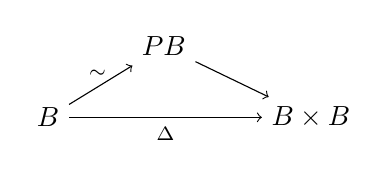
\begin{tikzpicture}[x=1.9em,y=1.35em]
    \node (pb) at (2.2,1.9) {$PB$};
    \node (b) at (0,0) {$B$};
    \node (bb) at (5.0,0) {$B\times B$};
    \draw[->] (b) -- node[above,pos=0.45]{$\scriptstyle\sim$} (pb);
    \draw[->] (pb) -- (bb);
    \draw[->] (b) -- node[below]{$\scriptstyle\Delta$} (bb);
  \end{tikzpicture}
  \end{center}
\item 一切对象都是\textbf{\trFibrant}{}的：对每个 $B\in\mathcal{M}$，映射
  $B\to 1$ 落于 $\rvF$ 中。
\end{enumerate}
\end{definition}

\begin{remark}\label{rem:original-definition}
原始定义在公理 (i) 中只要求有限\trProduct{}的存在性，并且省去了公理 (iv)。
类 $\rvF$ 与 $\rvF\cap\rvW$ 对有限\trProduct{}的封闭性，可由公理 (iii) 所
假设的对\trPullback{}的封闭性经归纳推得（见\cref{cor:finite-products}）。
在此，我们提出这些无穷\trLimit{}的要求，以与我们∞-\trInfinityCosmos{}定义中的%
\trLimit{}公理——第 1 章中的\cref{def:infinity-cosmos}(i)——相平行。实践中，
类 $\rvF$ 与 $\rvF\cap\rvW$ 常由一个右提升性质（right lifting property）
来刻画，此时封闭公理 (i)、(iii) 与 (iv) 自动成立（见\cref{lem:right-lifting-closure}）。
\end{remark}

一般而言，习惯上把 $\rvW$ 中的映射称作「\trWeakEquivalence」，把 $\rvF$ 中的
映射称作「\trFibration」，而把 $\rvF\cap\rvW$ 中的映射称作「\trTrivialFibration」
——除非具体语境要求别样的名称——并分别用装饰箭头
$\rvWarrow$、$\rvFarrow$ 与 $\rvTFarrow$ 来描绘这三个类。我们之所以对%
\trCategoryOfFibrantObjects{}怀有首要的兴趣，正是缘于以下两个例子。

\begin{example}\label{exa:cosmos-as-fibrant-objects}
一个\trInfinityCosmos{}的底范畴定义了一个\trCategoryOfFibrantObjects，其中取 $\rvW$ 为%
\trEquivalence{}类，$\rvF$ 为\trIsofibration{}类。\cref{def:category-of-fibrant-objects}
的多数公理已被第 1 章中的\cref{def:infinity-cosmos} 的\trLimit{}公理与%
\trIsofibration{}公理所涵盖；余下的部分则在\cref{lem:trivial-fibration-stability}、%
\cref{lem:equivalence-retracts-2-of-3} 与\cref{lem:brown-factorization}中建立。
\end{example}

\begin{example}\label{exa:model-category-fibrant-objects}
一个\trModelCategory{}中\trFibrant{}对象的全子范畴定义了一个\trCategoryOfFibrantObjects，
其中取 $\rvW$ 为\trWeakEquivalence{}类，$\rvF$ 为\trFibrant{}对象之间的%
\trFibration{}类（见\cref{def:fibrant-cofibrant} 与\cref{ex:fibrant-objects-from-model}）。
\end{example}

\begin{remark}\label{rem:right-proper}
刚刚讨论的两个例子都具有\textbf{\trRightProper}这一附加性质，即满足下面的%
一条附加公理：

(vii) $\rvW$ 中的映射沿 $\rvF$ 中映射的\trPullback{}仍是 $\rvW$ 中的映射：
\begin{center}
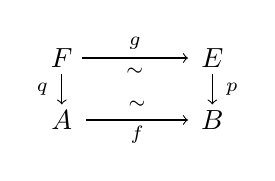
\begin{tikzpicture}[x=1.6em,y=1.6em]
  \node (tl) at (0,1.4) {$F$};
  \node (tr) at (3.4,1.4) {$E$};
  \node (bl) at (0,0) {$A$};
  \node (br) at (3.4,0) {$B$};
  \draw[->] (0.45,1.4) -- (2.85,1.4);
  \node at (1.65,1.74) {$\scriptstyle g$};
  \node at (1.65,1.1) {$\scriptstyle\sim$};
  \draw[->] (0,1.05) -- (0,0.35);
  \node at (-0.44,0.7) {$\scriptstyle q$};
  \node at (0.48,0.78) {$\scriptstyle\lrcorner$};
  \draw[->] (3.4,1.05) -- (3.4,0.35);
  \node at (3.84,0.7) {$\scriptstyle p$};
  \draw[->] (0.55,0) -- (2.85,0);
  \node at (1.7,-0.34) {$\scriptstyle f$};
  \node at (1.7,0.34) {$\scriptstyle\sim$};
\end{tikzpicture}
\end{center}
\end{remark}

对∞-宇宙而言，这在第 3 章中的\cref{prop:pullback-equivalence} 中得到证明；
而对模型范畴中的纤维性对象，这首先由 Reedy 在 \cite[Theorem B]{bib99} 中
观察到（另见 \cite[15.4.2]{bib84}）。

\trCategoryOfFibrantObjects{}中的分解公理可以推广，以构造任意映射的分解
（见第 1 章中的\cref{lem:brown-factorization}）。

\begin{lemma}[Brown 分解引理]\label{lem:brown-factorization-cfo}
\trCategoryOfFibrantObjects{}中的任何映射 $f\colon A\to B$ 都可以分解为一支%
\trWeakEquivalence{}继以一支\trFibration，其中该\trWeakEquivalence{}被%
构造为一支\trTrivialFibration{}的\trSection。
\begin{center}
\begin{tikzpicture}[x=1.6em,y=1.6em]
  \node (Pf) at (0.6,1.5) {$Pf$};
  \node (A) at (-1.4,0) {$A$};
  \node (B) at (3.0,0) {$B$};
  \draw[double,->] (Pf) to[bend right=28] node[pos=0.55,above,sloped]{$\scriptstyle\overset{\sim}{q}$} (A);
  \draw[->] (A) to[bend right=22] node[pos=0.5,below,sloped]{$\scriptstyle s$} (Pf);
  \draw[double,->] (Pf) -- node[pos=0.45,above,sloped]{$\scriptstyle p$} (B);
  \draw[->] (A) -- node[below]{$\scriptstyle f$} (B);
\end{tikzpicture}
\end{center}
此外，$f$ 是\trWeakEquivalence{}当且仅当\trFibration{} $p$ 是%
\trTrivialFibration。
\end{lemma}

\begin{proof}
图中所示的分解由 (v) 中\trPathObject{}分解 $B\rvWarrow PB\rvFarrow B\times B$
的\trPullback{}构造：
\begin{center}
\begin{tikzpicture}[x=1.6em,y=1.5em]
  \node (A) at (0,2.3) {$A$};
  \node (B) at (2.6,2.3) {$B$};
  \node (Pf) at (1.0,1.1) {$Pf$};
  \node (PB) at (2.9,1.1) {$PB$};
  \node (AB) at (0,0) {$A\times B$};
  \node (BB) at (3.5,0) {$B\times B$};
  \draw[->] (0.45,2.3) -- (2.1,2.3) node[midway,above]{$\scriptstyle f$};
  \draw[dashed,->] (0.1,2.0) -- (0.75,1.4) node[pos=0.4,left]{$\scriptstyle\overset{\sim}{s}$};
  \draw[->] (A) to[out=-105,in=115] node[pos=0.5,left]{$\scriptstyle(A,f)$} (AB);
  \draw[->] (0.8,0.85) -- (0.2,0.25) node[pos=0.45,left]{$\scriptstyle(q,p)$};
  \node at (1.35,0.85) {$\scriptstyle\lrcorner$};
  \draw[->] (1.35,1.1) -- (2.5,1.1);
  \draw[->] (2.7,2.0) -- (2.87,1.4) node[pos=0.45,left]{$\scriptstyle\sim$};
  \draw[->] (2.75,2.05) -- (3.4,0.25) node[pos=0.72,right]{$\scriptstyle\Delta$};
  \draw[double,->] (PB) -- (3.2,0.3);
  \draw[->] (0.55,0) -- (2.85,0) node[midway,below]{$\scriptstyle f\times B$};
\end{tikzpicture}
\end{center}
由\trWeakEquivalence{}的\trTwoOfThreeProperty，两支投影
$PB\rvTFarrow B$ 都是\trTrivialFibration。由于映射 $q$ 是这些投影之一沿
$f\colon A\to B$ 的\trPullback，由公理 (iii) 可知 $q$ 是\trTrivialFibration。
它的\trSection{} $s$——通过把\trPullback{}的\trUniversalProperty{}用于所示的
以 $A$ 为峰顶的\trCone{}而构造——因而是一支\trWeakEquivalence。最后，
若 $f$ 与 $p$ 中任何一个是\trWeakEquivalence，则由\trTwoOfThreeProperty，
另一个亦然。
\end{proof}

与第 1 章中的\cref{prop:sliced-cosmoi} 相类似：

\begin{corollary}\label{cor:slice-fibrant-objects}
若 $\mathcal{M}$ 是一个\trCategoryOfFibrantObjects{}且 $B\in\mathcal{M}$，则 $\mathcal{M}$
中余域为 $B$ 的诸\trFibration{}与其上 $B$ 的诸映射所构成的\trCategory{}
$\mathcal{M}_{/B}$ 成为一个\trCategoryOfFibrantObjects，其中\trWeakEquivalence{}与%
\trFibration{}由遗忘\trFunctor{} $\mathcal{M}_{/B}\to\mathcal{M}$ 所%
\textbf{创造}（created）。
\end{corollary}
\begin{proof}
切片\trCategory{} $\mathcal{M}_{/B}$ 中\trLimit{}的构造已在第 1 章中的%
\cref{prop:sliced-cosmoi} 之证明中描述；特别地，请注意 $\mathrm{id}_B$
是\trTerminal{}对象，故 $\mathcal{M}_{/B}$ 中的一切对象，作为 $\mathcal{M}$
中的\trFibration，都是\trFibrant{}的。\trFibration{} $f\colon A\rvFarrow B$
的诸\trPathObject{}可以这样构造：把\cref{lem:brown-factorization-cfo}
用于「对角」映射 $(f,f)\colon A\to A\times_B A$，即从 $A$ 到 $f$ 沿其
自身之\trPullback{}的映射。
\end{proof}

Blumberg 与 Mandell 的一个结果 \cite[6.4]{bib20} 之对偶表明：任何%
\trInfinityCosmos{}中的\trEquivalence{}都满足\trTwoOfSixProperty。其证明
揭示：这在任何\trCategoryOfFibrantObjects{}中都成立，只要类 $\rvW$ 对\trRetract{}封闭。%
\footnote{一条箭头 $f\colon A\to B$ 是一条箭头 $g\colon C\to D$ 的一个%
\textbf{\trRetract}，若存在\trDiagram：
\begin{center}
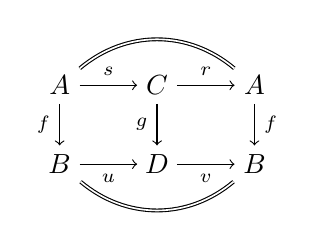
\begin{tikzpicture}[x=1.6em,y=1.5em]
  \node (At) at (0,1.3) {$A$};
  \node (C) at (2.2,1.3) {$C$};
  \node (Ar) at (4.4,1.3) {$A$};
  \node (B) at (0,-0.6) {$B$};
  \node (D) at (2.2,-0.6) {$D$};
  \node (Br) at (4.4,-0.6) {$B$};
  \draw[->] (0.45,1.3) -- (1.75,1.3) node[midway,above]{$\scriptstyle s$};
  \draw[->] (2.65,1.3) -- (3.95,1.3) node[midway,above]{$\scriptstyle r$};
  \draw[->] (0,0.85) -- (0,-0.15) node[midway,left]{$\scriptstyle f$};
  \draw[->] (2.2,0.85) -- (2.2,-0.15) node[midway,left]{$\scriptstyle g$};
  \draw[->] (4.4,0.85) -- (4.4,-0.15) node[midway,right]{$\scriptstyle f$};
  \draw[->] (0.45,-0.6) -- (1.75,-0.6) node[midway,below]{$\scriptstyle u$};
  \draw[->] (2.65,-0.6) -- (3.95,-0.6) node[midway,below]{$\scriptstyle v$};
  \draw[double] (At) to[out=40,in=140] (Ar);
  \draw[double] (B) to[out=-40,in=-140] (Br);
\end{tikzpicture}
\end{center}}

\begin{proposition}\label{prop:2-of-6-fibrant-objects}
设 $\mathcal{M}$ 是一个\trCategory，连同映射的两个类 $\rvW$ 与 $\rvF$，
使得：
\begin{itemize}
\item $\rvW$ 满足\trTwoOfThreeProperty，并且对\trRetract{}封闭。
\item $\rvF\cap\rvW$ 中一个映射的\trPullback{}仍在 $\rvF\cap\rvW$ 中，
  并且这些\trPullback{}总是存在。
\item $\rvW$ 中的每个映射都分解为某支 $\rvF\cap\rvW$ 中映射的\trSection{}%
  继以一支 $\rvF\cap\rvW$ 中的映射。
\end{itemize}
那么类 $\rvW$ 便满足\textbf{\trTwoOfSixProperty}：对任何可复合的三元组%
态射
\begin{center}
\begin{tikzpicture}[x=1.6em,y=1.5em]
  \node (A) at (0,0) {$A$};
  \node (B) at (2.2,1.4) {$B$};
  \node (D) at (4.4,0) {$D$};
  \node (C) at (2.2,-1.4) {$C$};
  \draw[->] (A) -- (B) node[pos=0.45,above,sloped]{$\scriptstyle f$};
  \draw[->] (B) -- (D) node[pos=0.45,above,sloped]{$\scriptstyle\overset{\sim}{hg}$};
  \draw[->] (A) -- (D) node[pos=0.5,above]{$\scriptstyle hgf$};
  \draw[->] (B) -- (C) node[pos=0.68,right]{$\scriptstyle g$};
  \draw[->] (A) -- (C) node[pos=0.6,below,sloped]{$\scriptstyle\overset{\sim}{gf}$};
  \draw[->] (C) -- (D) node[pos=0.5,below,sloped]{$\scriptstyle h$};
\end{tikzpicture}
\end{center}
若 $gf$ 与 $hg$ 属于类 $\rvW$，则 $f$、$g$、$h$ 与 $hgf$ 亦然。
\end{proposition}

\begin{proof}
对下方左侧所示的\trWeakEquivalence{} $hg$ 作分解，并作出 $p$ 沿 $h$ 的%
\trPullback{}与诱导映射 $t$：
\begin{center}
\begin{tikzpicture}[x=1.6em,y=1.5em]
  \node (Dp) at (2.6,1.3) {$D'$};
  \node (B) at (0,0) {$B$};
  \node (D) at (5.0,0) {$D$};
  \draw[->] (Dp) to[bend right=22] node[pos=0.5,above,sloped]{$\scriptstyle\overset{\sim}{r}$} (B);
  \draw[->] (B) to[bend right=18] node[pos=0.5,below,sloped]{$\scriptstyle\overset{\sim}{j}$} (Dp);
  \draw[double,->] (Dp) -- node[pos=0.5,above,sloped]{$\scriptstyle p$} (D);
  \draw[->] (B) -- (D) node[midway,below]{$\scriptstyle\overset{\sim}{hg}$};
\end{tikzpicture}
\qquad
\begin{tikzpicture}[x=1.6em,y=1.5em]
  \node (A) at (0,2.3) {$A$};
  \node (B) at (2.4,2.3) {$B$};
  \node (Cp) at (4.6,1.15) {$C'$};
  \node (Dp) at (6.4,1.15) {$D'$};
  \node (Br) at (8.8,1.15) {$B$};
  \node (C) at (3.8,-0.4) {$C$};
  \node (D) at (6.4,-0.4) {$D$};
  \draw[->] (A) -- (B) node[midway,above]{$\scriptstyle f$};
  \draw[dashed,->] (B) to[bend left=12] node[pos=0.55,above]{$\scriptstyle t$} (Cp);
  \draw[->] (B) to[bend left=18] node[pos=0.6,above,sloped]{$\scriptstyle\overset{\sim}{j}$} (Dp);
  \draw[->] (B) to[out=-95,in=45] node[pos=0.55,left]{$\scriptstyle g$} (C);
  \draw[->] (A) to[out=-80,in=160] node[pos=0.6,left]{$\scriptstyle\overset{\sim}{gf}$} (C);
  \draw[->] (Cp) -- (Dp) node[midway,above]{$\scriptstyle u$};
  \draw[->] (4.45,0.9) -- (4.45,0.05) node[midway,left]{$\scriptstyle q$};
  \node at (4.95,0.78) {$\scriptstyle\lrcorner$};
  \draw[->] (Dp) -- (Br) node[midway,above]{$\scriptstyle\overset{\sim}{r}$};
  \draw[double,->] (Dp) -- (D) node[midway,right]{$\scriptstyle p$};
  \draw[->] (C) -- (D) node[midway,below]{$\scriptstyle h$};
  \draw[double] (B) to[out=28,in=140] (Br);
\end{tikzpicture}
\end{center}
由\trTrivialFibration{}的\trPullback{}稳定性，映射 $q$ 属于 $\rvW$，于是由%
\trTwoOfThreeProperty{}及 $gf$ 属于 $\rvW$ 的假设，复合 $tf\colon A\to C'$
必属于 $\rvW$。映射 $f$ 是这一复合的一个\trRetract
\begin{center}
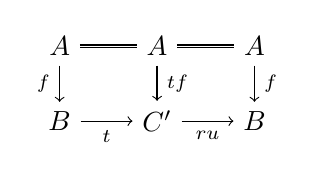
\begin{tikzpicture}[x=1.6em,y=1.5em]
  \node (A1) at (0,1.2) {$A$};
  \node (A2) at (2.2,1.2) {$A$};
  \node (A3) at (4.4,1.2) {$A$};
  \node (B) at (0,-0.6) {$B$};
  \node (Cp) at (2.2,-0.6) {$C'$};
  \node (B2) at (4.4,-0.6) {$B$};
  \draw[double] (A1) -- (A2);
  \draw[double] (A2) -- (A3);
  \draw[->] (A1) -- (B) node[midway,left]{$\scriptstyle f$};
  \draw[->] (A2) -- (Cp) node[midway,right]{$\scriptstyle tf$};
  \draw[->] (A3) -- (B2) node[midway,right]{$\scriptstyle f$};
  \draw[->] (B) -- (Cp) node[midway,below]{$\scriptstyle t$};
  \draw[->] (Cp) -- (B2) node[midway,below]{$\scriptstyle ru$};
\end{tikzpicture}
\end{center}
于是由类 $\rvW$ 的\trRetract{}封闭性，$f$ 属于 $\rvW$。现在由%
\trTwoOfThreeProperty{}即可进一步得出 $g$、$h$ 与 $hgf$ 都居于 $\rvW$ 中。
\end{proof}

\begin{corollary}\label{cor:2-of-6}
一个\trInfinityCosmos{}中的诸\trEquivalence{}满足\trTwoOfSixProperty。
\end{corollary}

\begin{proof}
只剩下论证\cref{prop:2-of-6-fibrant-objects} 的前提对任何\trInfinityCosmos{}%
中\trEquivalence{}、\trIsofibration{}与\trTrivialFibration{}的诸类成立。
第 1 章中的\cref{lem:equivalence-retracts-2-of-3} 证明：\trInfinityCosmos{}%
中的诸\trEquivalence{}还对\trRetract{}封闭并具有\trTwoOfThreeProperty。
第 1 章中的\cref{lem:trivial-fibration-stability} 证明：\trTrivialFibration{}%
类在\trPullback{}下稳定，而这些\trPullback{}在任何\trInfinityCosmos{}中都
存在。第 1 章中的\cref{lem:brown-factorization} 构造了所需的分解，由%
\trTwoOfThreeProperty，它把一个\trEquivalence{}分解为一支\trTrivialFibration{}%
的\trSection{}继以一支\trTrivialFibration。现在\cref{prop:2-of-6-fibrant-objects}
便适用于证明：任何\trInfinityCosmos{}中的诸\trEquivalence{}满足更强的%
\trTwoOfSixProperty。
\end{proof}

下述\cref{lem:brown-factorization-cfo} 的推论，传统上称作「Ken Brown 引理」，是证明%
\trCategoryOfFibrantObjects{}中种种\trLimit{}构造在\trPointwise{}\trWeakEquivalence{}之下
的不变性的关键所在。

\begin{lemma}[Ken Brown 引理]\label{lem:ken-brown}
考虑一个\trFunctor{} $F\colon\mathcal{M}\to\mathcal{N}$：其定义域是一个%
\trCategoryOfFibrantObjects，其陪域是一个配有满足\trTwoOfThreeProperty{}的
「\trWeakEquivalence」子范畴的\trCategory。若 $F$ 把\trTrivialFibration{}载为%
\trWeakEquivalence，则 $F$ 把 $\mathcal{M}$ 中的\trWeakEquivalence{}载为
$\mathcal{N}$ 中的\trWeakEquivalence。
\end{lemma}

\begin{proof}
由\cref{lem:brown-factorization-cfo}，\trCategoryOfFibrantObjects{}中的任何%
\trWeakEquivalence{}都可以分解为一支\trTrivialFibration{}的\trSection{}继以
一支\trTrivialFibration。
\begin{center}
\begin{tikzpicture}[x=1.6em,y=1.6em]
  \node (Pf) at (0.6,1.5) {$Pf$};
  \node (A) at (-1.4,0) {$A$};
  \node (B) at (3.0,0) {$B$};
  \draw[double,->] (Pf) to[bend right=28] node[pos=0.55,above,sloped]{$\scriptstyle\overset{\sim}{q}$} (A);
  \draw[->] (A) to[bend right=22] node[pos=0.5,below,sloped]{$\scriptstyle s$} (Pf);
  \draw[double,->] (Pf) -- node[pos=0.45,above,sloped]{$\scriptstyle p$} (B);
  \draw[->] (A) -- node[below]{$\scriptstyle\overset{\sim}{f}$} (B);
\end{tikzpicture}
\end{center}
由假设，映射 $q$ 与 $p$ 在 $F$ 之下的像是\trWeakEquivalence。由 $\mathcal{N}$
中\trWeakEquivalence{}的\trTwoOfThreeProperty，即可得出：$s$ 的像、从而
也有 $f$ 的像，都是\trWeakEquivalence。
\end{proof}

本节其余部分致力于\cref{lem:ken-brown} 的种种应用，以确立\trCategoryOfFibrantObjects{}%
中诸\trLimit{}的\trWeakEquivalence{}不变性。

\begin{lemma}\label{lem:pullback-we-between-fibrations}
在\trCategoryOfFibrantObjects{}中，诸\trFibration{}之间的一个\trWeakEquivalence{}拉回为
诸\trFibration{}之间的一个\trWeakEquivalence：
\begin{center}
\begin{tikzpicture}[x=1.6em,y=1.5em]
  \node (P) at (0,2) {$P$};
  \node (E) at (3.2,2) {$E$};
  \node (Q) at (1.2,1) {$Q$};
  \node (F) at (3.6,1) {$F$};
  \node (A) at (0,0) {$A$};
  \node (B) at (2.8,0) {$B$};
  \draw[->] (P) -- (E);
  \draw[->] (0.4,1.75) -- (1.05,1.28) node[pos=0.4,right]{$\scriptstyle u$};
  \node at (0.5,1.62) {$\scriptstyle\lrcorner$};
  \draw[->] (Q) -- (F);
  \draw[->] (0,1.7) -- (0,0.3) node[midway,left]{$\scriptstyle r$};
  \draw[->] (1.05,0.75) -- (0.4,0.26) node[pos=0.55,below]{$\scriptstyle s$};
  \node at (1.7,0.62) {$\scriptstyle\lrcorner$};
  \draw[double,->] (3.2,1.7) -- (3.2,0.3) node[midway,left]{$\scriptstyle p$};
  \draw[double,->] (3.75,0.7) -- (3.05,0.06) node[pos=0.6,right]{$\scriptstyle q$};
  \draw[->] (2.75,1.85) -- (3.35,1.28) node[pos=0.5,right]{$\scriptstyle\overset{\sim}{e}$};
  \draw[->] (0.55,0) -- (2.25,0) node[midway,below]{$\scriptstyle\overset{\sim}{f}$};
\end{tikzpicture}
\end{center}
\end{lemma}

\begin{proof}
由\cref{cor:slice-fibrant-objects}，\trCategoryOfFibrantObjects{} $\mathcal{M}$ 的诸切片
定义\trCategoryOfFibrantObjects，而且沿 $f$ 的\trPullback{}定义了一个\trFunctor{}
$f^{\ast}\colon\mathcal{M}_{/B}\to\mathcal{M}_{/A}$。注意所示\trDiagram{}中的映射
$u$ 是映射 $e$ 的\trPullback，于是由\cref{def:category-of-fibrant-objects}
的公理 (iii) 直接可得：拉回保持\trTrivialFibration。于是\cref{lem:ken-brown}
蕴含：它也保持诸\trEquivalence。
\end{proof}

类似脉络的其他结果则需要些许更为精致的论证。下面给出的证明原本归于
Reedy 的一部未出版手稿 \cite{bib99}，这部手稿隐含地孕育了我们在 C.4 节中
引入的「Reedy 范畴」概念。

\begin{proposition}\label{prop:pullback-map-fibration}
考虑\trCategoryOfFibrantObjects{}中的一个\trDiagram：
\begin{center}
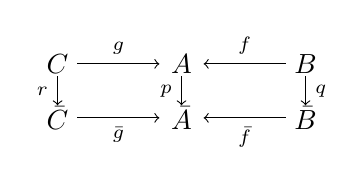
\begin{tikzpicture}[x=1.6em,y=1.5em]
  \node (C) at (0,1.3) {$C$};
  \node (A) at (2.8,1.3) {$A$};
  \node (B) at (5.6,1.3) {$B$};
  \node (Cb) at (0,0) {$\bar{C}$};
  \node (Ab) at (2.8,0) {$\bar{A}$};
  \node (Bb) at (5.6,0) {$\bar{B}$};
  \draw[->] (0.45,1.3) -- (2.3,1.3) node[midway,above]{$\scriptstyle g$};
  \draw[->] (5.15,1.3) -- (3.3,1.3) node[midway,above]{$\scriptstyle f$};
  \draw[->] (0,1.0) -- (0,0.3) node[midway,left]{$\scriptstyle r$};
  \draw[->] (2.8,1.0) -- (2.8,0.3) node[midway,left]{$\scriptstyle p$};
  \draw[->] (5.6,1.0) -- (5.6,0.3) node[midway,right]{$\scriptstyle q$};
  \draw[->] (0.45,0) -- (2.3,0) node[midway,below]{$\scriptstyle\bar{g}$};
  \draw[->] (5.15,0) -- (3.3,0) node[midway,below]{$\scriptstyle\bar{f}$};
\end{tikzpicture}
\end{center}
若映射 $r$ 与映射 $z\colon B\to A\times_{\bar{A}}\bar{B}$ 都是\trFibration{}或
都是\trTrivialFibration，那么从 $f$ 沿 $g$ 的\trPullback{}到 $\bar{f}$ 沿
$\bar{g}$ 的\trPullback{}的诱导映射，相应地仍是\trFibration{}或%
\trTrivialFibration。
\end{proposition}

\begin{proof}
由\trPullback{}的复合与消去，诱导映射 $t$ 分解为 $z$ 的一个\trPullback{}继以 $r$
的一个\trPullback，如下面所示
\begin{center}
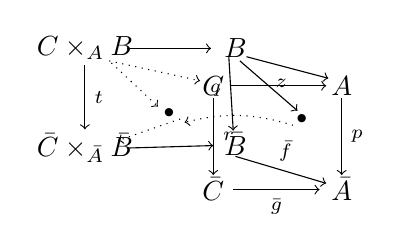
\begin{tikzpicture}[x=1.6em,y=1.5em]
  \node (CB) at (0,2.4) {$C\times_A B$};
  \node (B) at (3.4,2.4) {$B$};
  \node (A) at (5.8,1.5) {$A$};
  \node (C) at (2.9,1.5) {$C$};
  \node (d1) at (1.9,0.85) {$\scriptstyle\bullet$};
  \node (d2) at (4.9,0.7) {$\scriptstyle\bullet$};
  \node (CBb) at (0,0) {$\bar{C}\times_{\bar{A}}\bar{B}$};
  \node (Bb) at (3.4,0.1) {$\bar{B}$};
  \node (Cb) at (2.9,-1.0) {$\bar{C}$};
  \node (Ab) at (5.8,-1.0) {$\bar{A}$};
  \draw[->] (0.95,2.4) -- (2.85,2.4);
  \draw[dotted,->] (0.55,2.1) -- (2.6,1.62);
  \draw[dotted,->] (0.6,2.05) -- (1.65,1.0);
  \draw[->] (0,2.0) -- (0,0.45) node[midway,right]{$\scriptstyle t$};
  \draw[->] (3.65,2.2) -- (5.5,1.68);
  \draw[->] (3.3,1.5) -- (5.45,1.5);
  \draw[->] (3.5,2.1) -- (4.8,0.9) node[pos=0.45,right]{$\scriptstyle z$};
  \draw[->] (3.25,2.2) -- (3.35,0.42) node[pos=0.45,left]{$\scriptstyle q$};
  \draw[->] (2.9,1.2) -- (2.9,-0.65) node[midway,right]{$\scriptstyle r$};
  \draw[->] (5.8,1.2) -- (5.8,-0.65) node[midway,right]{$\scriptstyle p$};
  \node at (2.2,0.6) {$\scriptstyle\lrcorner$};
  \node at (5.2,0.45) {$\scriptstyle\lrcorner$};
  \draw[dotted,->] (2.15,0.7) -- (0.75,0.18);
  \draw[dotted,->] (4.7,0.55) to[bend right=15] (2.25,0.62);
  \draw[->] (0.95,0) -- (2.9,0.06);
  \draw[->] (3.4,-0.2) -- (5.45,-0.85) node[pos=0.55,above]{$\scriptstyle\bar{f}$};
  \draw[->] (3.35,-1.0) -- (5.3,-1.0) node[midway,below]{$\scriptstyle\bar{g}$};
\end{tikzpicture}
\end{center}
于是当这两支映射都是\trFibration{}或都是\trTrivialFibration{}时，它亦然。
\end{proof}

类似地，我们有如下结果，其对偶形式有时称作「\textbf{粘合引理}」
（gluing lemma）。

\begin{proposition}\label{prop:pullback-map-equivalence}
在一个\trCategoryOfFibrantObjects{}中，如下形式之\trDiagram{}的两个水平行各自的%
\trPullback{}之间的诱导映射仍是一个\trWeakEquivalence：
\begin{center}
\begin{tikzpicture}[x=1.6em,y=1.5em]
  \node (C) at (0,1.3) {$C$};
  \node (A) at (2.8,1.3) {$A$};
  \node (B) at (5.6,1.3) {$B$};
  \node (Cb) at (0,0) {$\bar{C}$};
  \node (Ab) at (2.8,0) {$\bar{A}$};
  \node (Bb) at (5.6,0) {$\bar{B}$};
  \draw[->] (0.45,1.3) -- (2.3,1.3) node[midway,above]{$\scriptstyle g$};
  \draw[->] (5.15,1.3) -- (3.3,1.3) node[midway,above]{$\scriptstyle f$};
  \draw[->] (0,1.0) -- (0,0.3) node[midway,left]{$\scriptstyle\overset{\sim}{r}$};
  \draw[->] (2.8,1.0) -- (2.8,0.3) node[midway,left]{$\scriptstyle\overset{\sim}{p}$};
  \draw[->] (5.6,1.0) -- (5.6,0.3) node[midway,right]{$\scriptstyle\overset{\sim}{q}$};
  \draw[->] (0.45,0) -- (2.3,0) node[midway,below]{$\scriptstyle\bar{g}$};
  \draw[->] (5.15,0) -- (3.3,0) node[midway,below]{$\scriptstyle\bar{f}$};
\end{tikzpicture}
\end{center}
\end{proposition}

第 3 章中的\cref{prop:pullback-invariance} 的证明同样适用于任何%
\trRightProper{}\trCategoryOfFibrantObjects，但正如我们将发现的，\trRightProperness{}%
这一假设实际上并不必要。

\begin{proof}
由\cref{ex:cospan-cfo}，对任何\trCategoryOfFibrantObjects{} $\mathcal{M}$ 都存在一个%
\trCategoryOfFibrantObjects{} $\mathcal{M}^{\perp}$，其
\begin{itemize}
\item 对象是\trCospan{} $C\xrightarrow{g}A\xleftarrow{f}B$，其中右腿是
  $\mathcal{M}$ 中的一支\trFibration；
\item \trWeakEquivalence{}是\trPointwise{}\trWeakEquivalence；并且
\item \trFibration{}是形如下图的\trDiagram，其中映射 $r$、$p$ 与 $q$
  都是\trFibration，而诱导映射 $z\colon B\to A\times_{\bar{A}}\bar{B}$
  亦然：
\begin{center}
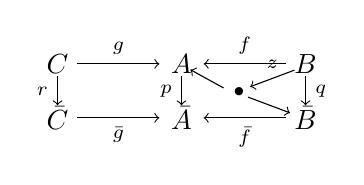
\begin{tikzpicture}[x=1.6em,y=1.5em]
  \node (C) at (0,1.3) {$C$};
  \node (A) at (2.8,1.3) {$A$};
  \node (B) at (5.6,1.3) {$B$};
  \node (Cb) at (0,0) {$\bar{C}$};
  \node (Ab) at (2.8,0) {$\bar{A}$};
  \node (Bb) at (5.6,0) {$\bar{B}$};
  \node (dot) at (4.1,0.62) {$\scriptstyle\bullet$};
  \draw[->] (0.45,1.3) -- (2.3,1.3) node[midway,above]{$\scriptstyle g$};
  \draw[->] (5.15,1.3) -- (3.3,1.3) node[midway,above]{$\scriptstyle f$};
  \draw[->] (0,1.0) -- (0,0.3) node[midway,left]{$\scriptstyle r$};
  \draw[->] (2.8,1.0) -- (2.8,0.3) node[midway,left]{$\scriptstyle p$};
  \draw[->] (5.6,1.0) -- (5.6,0.3) node[midway,right]{$\scriptstyle q$};
  \draw[->] (0.45,0) -- (2.3,0) node[midway,below]{$\scriptstyle\bar{g}$};
  \draw[->] (5.15,0) -- (3.3,0) node[midway,below]{$\scriptstyle\bar{f}$};
  \draw[->] (5.35,1.15) -- (4.35,0.75) node[pos=0.5,above]{$\scriptstyle z$};
  \draw[->] (3.75,0.72) -- (3.0,1.16);
  \draw[->] (4.3,0.5) -- (5.25,0.12);
  \node at (4.42,0.5) {$\scriptstyle\lrcorner$};
\end{tikzpicture}
\end{center}
\end{itemize}
而所需的诸\trLimit{}则逐点继承自 $\mathcal{M}$。由%
\cref{prop:pullback-map-fibration}，拉回\trFunctor{}
$\lim\colon\mathcal{M}^{\perp}\to\mathcal{M}$ 把\trTrivialFibration{}载为%
\trTrivialFibration，于是由\cref{lem:ken-brown}，它也保持诸%
\trWeakEquivalence。
\end{proof}

\begin{corollary}\label{cor:finite-products}
在一个\trCategoryOfFibrantObjects{}中，诸\trFibration{}、诸\trTrivialFibration{}或诸%
\trWeakEquivalence{}的有限\trProduct{}仍是\trFibration{}、%
\trTrivialFibration{}或\trWeakEquivalence。
\end{corollary}

\begin{proof}
一族有限多个映射 $\{f_i\colon A_i\to\bar{A}_i\}_{i=1,\dots,n}$ 的\trProduct{}%
可以归纳地构造为\trTerminal{}对象 $1$ 上的一个\trPullback：
\begin{center}
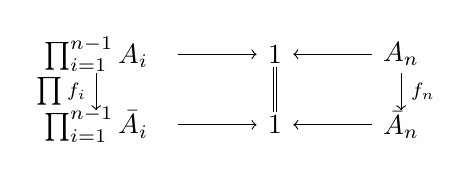
\begin{tikzpicture}[x=1.9em,y=1.5em]
  \node (P1) at (0,1.3) {$\prod\nolimits_{i=1}^{n-1}A_i$};
  \node (1t) at (3.4,1.3) {$1$};
  \node (An) at (5.8,1.3) {$A_n$};
  \node (P2) at (0,-0.4) {$\prod\nolimits_{i=1}^{n-1}\bar{A}_i$};
  \node (1b) at (3.4,-0.4) {$1$};
  \node (Anb) at (5.8,-0.4) {$\bar{A}_n$};
  \draw[->] (1.55,1.3) -- (3.05,1.3);
  \draw[->] (5.25,1.3) -- (3.75,1.3);
  \draw[->] (0,0.85) -- (0,-0.05) node[midway,left]{$\scriptstyle\prod f_i$};
  \draw[double] (3.4,1.0) -- (3.4,-0.1);
  \draw[->] (5.8,0.85) -- (5.8,-0.05) node[midway,right]{$\scriptstyle f_n$};
  \draw[->] (1.55,-0.4) -- (3.05,-0.4);
  \draw[->] (5.25,-0.4) -- (3.75,-0.4);
\end{tikzpicture}
\end{center}
当每个映射 $f_i$ 都是\trFibration{}或\trTrivialFibration{}时，由%
\cref{prop:pullback-map-fibration}及从二元\trProduct{}情形起步的归纳，
这些映射的\trProduct{}亦然。当每个映射 $f_i$ 都是\trWeakEquivalence{}时，
同样的结论由\cref{prop:pullback-map-equivalence} 得出。
\end{proof}

类似地，诸\trFibration{}之塔的诸\trLimit{}在\trPointwise{}%
\trWeakEquivalence{}下不变：

\begin{proposition}\label{prop:tower-limits}
考虑\trCategoryOfFibrantObjects{}中诸可数\trFibration{}塔之间的一个\trNaturalTransformation
\begin{center}
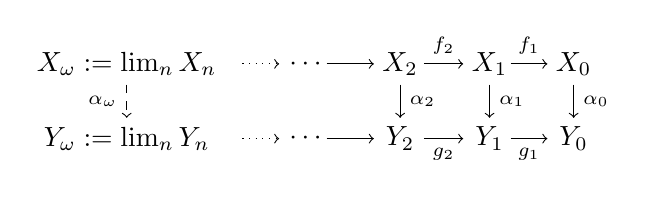
\begin{tikzpicture}[x=1.9em,y=1.5em]
  \node (Xw) at (0,1.3) {$X_\omega:=\lim_n X_n$};
  \node (Xd) at (3.4,1.3) {$\cdots$};
  \node (X2) at (5.2,1.3) {$X_2$};
  \node (X1) at (6.9,1.3) {$X_1$};
  \node (X0) at (8.5,1.3) {$X_0$};
  \node (Yw) at (0,-0.5) {$Y_\omega:=\lim_n Y_n$};
  \node (Yd) at (3.4,-0.5) {$\cdots$};
  \node (Y2) at (5.2,-0.5) {$Y_2$};
  \node (Y1) at (6.9,-0.5) {$Y_1$};
  \node (Y0) at (8.5,-0.5) {$Y_0$};
  \draw[dotted,->] (2.2,1.3) -- (2.9,1.3);
  \draw[->] (3.8,1.3) -- (4.7,1.3);
  \draw[->] (5.65,1.3) -- (6.4,1.3) node[midway,above]{$\scriptstyle f_2$};
  \draw[->] (7.3,1.3) -- (8.0,1.3) node[midway,above]{$\scriptstyle f_1$};
  \draw[dotted,->] (2.2,-0.5) -- (2.9,-0.5);
  \draw[->] (3.8,-0.5) -- (4.7,-0.5);
  \draw[->] (5.65,-0.5) -- (6.4,-0.5) node[midway,below]{$\scriptstyle g_2$};
  \draw[->] (7.3,-0.5) -- (8.0,-0.5) node[midway,below]{$\scriptstyle g_1$};
  \draw[dashed,->] (0,0.8) -- (0,-0.0) node[midway,left]{$\scriptstyle\alpha_\omega$};
  \draw[->] (5.2,0.8) -- (5.2,0.0) node[midway,right]{$\scriptstyle\alpha_2$};
  \draw[->] (6.9,0.8) -- (6.9,0.0) node[midway,right]{$\scriptstyle\alpha_1$};
  \draw[->] (8.5,0.8) -- (8.5,0.0) node[midway,right]{$\scriptstyle\alpha_0$};
\end{tikzpicture}
\end{center}
\begin{enumerate}[label=(\roman*)]
\item 若对每个 $n\geq 0$，映射
  $\langle\alpha_n,f_n\rangle\colon X_n\to Y_n\times_{Y_{n-1}}X_{n-1}$
  是\trFibration{}或\trTrivialFibration，\footnote{为使 $n=0$ 的情形有
  意义，约定 $X_{-1}$ 与 $Y_{-1}$ 为\trTerminal{}对象，于是此时所考虑的
  映射即 $\alpha_0$。}那么诸\trLimit{}之间的诱导映射 $\alpha_\omega$
  亦然。
\item 若对每个 $n\geq 0$，映射 $\alpha_n$ 是\trWeakEquivalence，那么诸%
  \trLimit{}之间的诱导映射 $\alpha_\omega$ 亦然。
\end{enumerate}
\end{proposition}

\begin{proof}
当 (i) 的假设在\trCategoryOfFibrantObjects{} $\mathcal{M}$ 中成立时，诸\trFibration{}塔之
诸\trLimit{}之间的诱导映射 $\alpha_\omega\colon X_\omega\to Y_\omega$
本身就是下述\trFibration{}塔或\trTrivialFibration{}塔的一个极限复合
\begin{center}
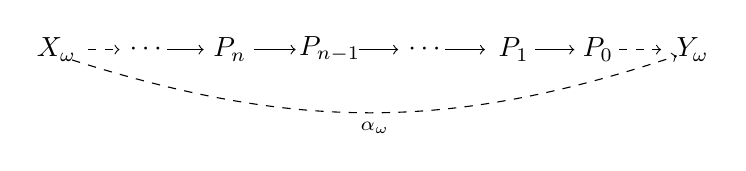
\begin{tikzpicture}[x=1.9em,y=1.5em]
  \node (Xw) at (0,0) {$X_\omega$};
  \node (D1) at (1.7,0) {$\cdots$};
  \node (Pn) at (3.3,0) {$P_n$};
  \node (Pn1) at (5.2,0) {$P_{n-1}$};
  \node (D2) at (7.0,0) {$\cdots$};
  \node (P1) at (8.7,0) {$P_1$};
  \node (P0) at (10.3,0) {$P_0$};
  \node (Yw) at (12.1,0) {$Y_\omega$};
  \draw[dashed,->] (0.6,0) -- (1.2,0);
  \draw[->] (2.1,0) -- (2.8,0);
  \draw[->] (3.75,0) -- (4.55,0);
  \draw[->] (5.75,0) -- (6.5,0);
  \draw[->] (7.4,0) -- (8.15,0);
  \draw[->] (9.1,0) -- (9.85,0);
  \draw[dashed,->] (10.7,0) -- (11.5,0);
  \draw[dashed,->] (0.3,-0.25) to[bend right=18] node[pos=0.5,below]{$\scriptstyle\alpha_\omega$} (11.8,-0.15);
\end{tikzpicture}
\end{center}
其中每一层都是下述映射的一个\trPullback，而该映射被假设为\trFibration{}或%
\trTrivialFibration：
\begin{center}
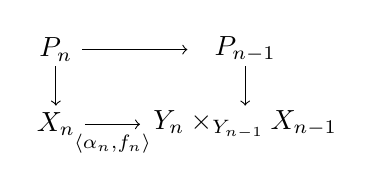
\begin{tikzpicture}[x=1.9em,y=1.5em]
  \node (Pn) at (0,1.2) {$P_n$};
  \node (Pn1) at (3.6,1.2) {$P_{n-1}$};
  \node (Xn) at (0,-0.6) {$X_n$};
  \node (YX) at (3.6,-0.6) {$Y_n\times_{Y_{n-1}}X_{n-1}$};
  \draw[->] (0.5,1.2) -- (2.5,1.2);
  \node at (0.55,0.9) {$\scriptstyle\lrcorner$};
  \draw[->] (0,0.8) -- (0,-0.15);
  \draw[->] (3.6,0.8) -- (3.6,-0.15);
  \draw[->] (0.55,-0.6) -- (1.6,-0.6) node[midway,below]{$\scriptstyle\langle\alpha_n,f_n\rangle$};
\end{tikzpicture}
\end{center}
从底部开始，$P_0$ 定义为 $\alpha_0$ 沿 $Y_\omega$ 的\trLimit{}\trCone{}%
的一条腿的\trPullback：
\begin{center}
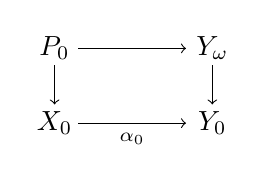
\begin{tikzpicture}[x=1.9em,y=1.5em]
  \node (P0) at (0,1.2) {$P_0$};
  \node (Yw) at (3.0,1.2) {$Y_\omega$};
  \node (X0) at (0,-0.6) {$X_0$};
  \node (Y0) at (3.0,-0.6) {$Y_0$};
  \draw[->] (0.45,1.2) -- (2.5,1.2);
  \node at (0.55,0.9) {$\scriptstyle\lrcorner$};
  \draw[->] (0,0.8) -- (0,-0.15);
  \draw[->] (3.0,0.8) -- (3.0,-0.15);
  \draw[->] (0.45,-0.6) -- (2.5,-0.6) node[midway,below]{$\scriptstyle\alpha_0$};
\end{tikzpicture}
\end{center}
由构造，$P_0$ 容许一个到\trPullback{} $Y_1\times_{Y_0}X_0$ 的\trCanonical{}%
映射，而 $P_1$ 被定义为如下\trPullback：
\begin{center}
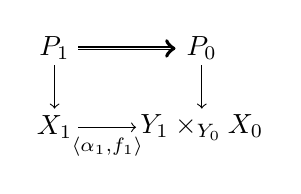
\begin{tikzpicture}[x=1.9em,y=1.5em]
  \node (P1) at (0,1.2) {$P_1$};
  \node (P0) at (2.8,1.2) {$P_0$};
  \node (X1) at (0,-0.7) {$X_1$};
  \node (YX) at (2.8,-0.7) {$Y_1\times_{Y_0}X_0$};
  \draw[double,->] (0.45,1.2) -- (2.3,1.2);
  \node at (0.55,0.9) {$\scriptstyle\lrcorner$};
  \draw[->] (0,0.8) -- (0,-0.25);
  \draw[->] (2.8,0.8) -- (2.8,-0.25);
  \draw[->] (0.45,-0.7) -- (1.55,-0.7) node[midway,below]{$\scriptstyle\langle\alpha_1,f_1\rangle$};
\end{tikzpicture}
\end{center}
继续归纳地做下去，诸\trFibration{}的塔
$P_n\rvFarrow P_{n-1}$ 的\trLimit{}可以被看出与 $\omega^{\mathrm{op}}\times 2$
形状的\trDiagram{}之\trLimit{}相重合，该\trDiagram{}由映射 $f_n$、$g_n$ 与 $\alpha_n$
构成。由于此\trDiagram{}顶行的包含
$\omega^{\mathrm{op}}\hookrightarrow\omega^{\mathrm{op}}\times 2$
是始的，这个\trLimit{}复原出 $X_\omega$，而诸\trFibration{}之塔的复合
复原出映射 $\alpha_\omega$。于是，由\cref{def:category-of-fibrant-objects}
的公理 (iii) 与 (iv)，诱导映射 $\alpha_\omega$ 相应地仍是\trFibration{}或%
\trTrivialFibration。

第二个陈述现在这样得出：把\cref{lem:ken-brown} 用于\trLimit{}\trFunctor{}
$\lim\colon\mathcal{M}^{\omega^{\mathrm{op}}}\to\mathcal{M}$，其定义域是诸%
\trFibration{}塔的\trCategory{}（见\cref{ex:towers-cfo}）。
\end{proof}

在这个证明中，我们再一次利用了这样一个事实：取值于\trCategoryOfFibrantObjects{}的%
\trDiagram{}\trCategory{}自身也可以配备\trCategoryOfFibrantObjects{}的结构——至少对某些
类型的\trDiagram{}与某些\trDiagram{}形状是如此。我们现在对一个格外有用的%
\trDiagram{}族——即以\textbf{逆范畴}（inverse categories）为标的%
\trDiagram{}——更系统地确立这一结果。

\begin{definition}\label{def:inverse-category}
一个\trCategory{} $\mathcal{J}$ 是一个\textbf{逆范畴}（inverse category），
若存在一个\trFunctor{} $\mathrm{deg}\colon\mathcal{J}\to\omega^{\mathrm{op}}$
使其反映恒同。\footnote{若把 $\omega$ 换成\trOrdinalCategory，数学内容并无
实质性改变。我们限制于有限度数的原因在于：\cref{def:category-of-fibrant-objects}
只要求 $\omega^{\mathrm{op}}$ 标引的塔之\trLimit{}（见\cref{prop:general-towers}(i)）。}
\end{definition}

度函子给 $\mathcal{J}$ 的每个对象指派一个自然数度数，使得一切非恒同态射
都「降低度数」——也就是说，其定义域对象的度数严格大于其陪域对象的
度数。度函子之于逆范畴的用处在于：它使我们得以归纳地指定以度数有界之
对象的诸全子范畴
\begin{center}
\begin{tikzpicture}[x=2.1em,y=1.4em]
  \node (J0) at (0,0) {$\mathcal{J}_{\leq 0}$};
  \node (D1) at (1.8,0) {$\cdots$};
  \node (Jn1) at (3.7,0) {$\mathcal{J}_{\leq n-1}$};
  \node (Jn) at (6.0,0) {$\mathcal{J}_{\leq n}$};
  \node (D2) at (7.8,0) {$\cdots$};
  \node (Jc) at (10.4,0) {$\operatorname{colim}_{n\in\omega}\mathcal{J}_{\leq n}\cong\mathcal{J}$};
  \draw[right hook->] (0.7,0) -- (1.35,0);
  \draw[right hook->] (2.25,0) -- (3.1,0);
  \draw[right hook->] (4.4,0) -- (5.35,0);
  \draw[right hook->] (6.65,0) -- (7.35,0);
  \draw[right hook->] (8.25,0) -- (9.1,0);
\end{tikzpicture}
\end{center}
为标的\trDiagram，从而定义一个 $\mathcal{J}$ 标引的\trDiagram{}或%
\trNaturalTransformation{}的数据。要把 $X\in\mathcal{M}^{\mathcal{J}_{\leq n-1}}$ 扩张为
$\mathcal{M}^{\mathcal{J}_{\leq n}}$ 中的一个\trDiagram，需要对每个度数为 $n$ 的
对象 $i$ 指定一个对象 $X^i\in\mathcal{M}$，连同
一支从 $X^i$ 指向如下\trLimit{}的映射 $X^i\to\partial^i X$：
\begin{rveq}\label{eq:boundary-object}
\partial^i X:=\operatorname{lim}_{i\to j}X_j
:=\operatorname{lim}\Big(\;
\underset{\textstyle i\ne j}{\mathcal{J}_{\leq n-1}}
\xrightarrow{\ \mathrm{cod}\ }
\mathcal{J}_{\leq n-1}
\xrightarrow{\ X\ }
\mathcal{M}\;\Big)
\end{rveq}
其以 $\mathcal{J}$ 中的非恒同映射 $i\to j$ 为标引。

\begin{observation}[边界数据作为一个\trWeightedLimit]\label{obs:boundary-weighted-limit}
正如记号所提示的那样，对象 $\partial^i X$ 应当被理解为与 $X^i$ 相关联的
「\trBoundary{}数据」之对象。这一直觉可以经由\trWeightedLimit{}的形式理论
而变得精确，这即便在非富集的语境中也例示了它们的用处。

回顾附录 A 中的\cref{def:weighted-limit-colimit-axiomatic}(i)：\trDiagram
$X\in\mathcal{M}^{\mathcal{J}}$ 在对象 $i\in\mathcal{J}$ 处被可表示函子
$\mathcal{J}(i,-)\in\mathcal{S}et^{\mathcal{J}}$ 加权的\trLimit{}即对象
$X^i$。把可表示函子的\textbf{\trBoundary}
$\partial\mathcal{J}(i,-)\in\mathcal{S}et^{\mathcal{J}}$ 定义为由下式给出的函子
\[
\partial\mathcal{J}(i,j):=\begin{cases}
\mathcal{J}(i,j) & \deg(j)<\deg(i)\\
\varnothing & \deg(j)\geq\deg(i)
\end{cases}
\]
将\eqref{eq:boundary-object} 与附录 A 中的%
\cref{rem:unenriched-indexing-categories} 的公式相比较，我们观察到
$\operatorname{lim}_{\partial\mathcal{J}(i,-)}X\cong\partial^i X$。

回顾附录 A 中的\cref{def:weighted-limit-colimit-axiomatic}：\trWeightedLimit{}%
对权是反变函子性的。于是，自然包含
$\partial\mathcal{J}(i,-)\hookrightarrow\mathcal{J}(i,-)$ 便诱导出一个%
\trCanonical{}映射
\[
X^i\cong\operatorname{lim}_{\mathcal{J}(i,-)}X
\xrightarrow{\ m^i\ }
\operatorname{lim}_{\partial\mathcal{J}(i,-)}X
\cong\partial^i X
\]
介于诸\trWeightedLimit{}之间。提前借用 C.4 节中\cref{def:latching-matching-objects}的术语，我们把
$\partial^i X$ 称作\trDiagram{} $X$ 的第 $i$ 个\textbf{匹配对象}，并把
$m^i\colon X^i\to\partial^i X$ 称作第 $i$ 个\textbf{匹配映射}。
\end{observation}

出于稍后便会明朗的原因，我们定义：

\begin{definition}\label{def:fibrant-diagram}
设 $\mathcal{M}$ 是一个\trCategoryOfFibrantObjects，并设 $\mathcal{J}$ 是一个逆范畴。
\begin{itemize}
\item 一个\textbf{纤维性图表}（fibrant diagram）是一个\trDiagram
  $X\in\mathcal{M}^{\mathcal{J}}$，它具有如下性质：对每个
  $i\in\mathcal{J}$，匹配映射 $m^i\colon X^i\to\partial^i X$
  是一个\trFibration。
\item 一个\textbf{纤维性自然变换}（fibrant natural transformation）是
  纤维性图表之间的一个\trNaturalTransformation{}
  $\alpha\colon X\to Y\in\mathcal{M}^{\mathcal{J}}$，使得对每个
  $i\in\mathcal{J}$，由诸匹配映射构成的方块中的\trPullback{}所定义的
  \textbf{相对匹配映射}（relative matching map）$\hat{m}^i$ 是一个%
  \trFibration：
\begin{rveq}\label{eq:relative-matching-map}
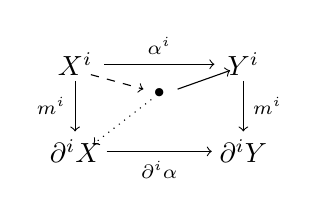
\begin{tikzpicture}[x=1.9em,y=1.5em]
  \node (Xi) at (0,1.2) {$X^i$};
  \node (Yi) at (3.2,1.2) {$Y^i$};
  \node (dot) at (1.6,0.5) {$\scriptstyle\bullet$};
  \node (dX) at (0,-0.9) {$\partial^i X$};
  \node (dY) at (3.2,-0.9) {$\partial^i Y$};
  \draw[->] (0.55,1.2) -- (2.65,1.2) node[midway,above]{$\scriptstyle\alpha^i$};
  \draw[dashed,->] (0.3,0.95) -- (1.3,0.6);
  \draw[->] (1.95,0.6) -- (2.95,1.05);
  \draw[dotted,->] (1.45,0.35) -- (0.35,-0.72);
  \node at (1.92,0.32) {$\scriptstyle\lrcorner$};
  \draw[->] (0,0.8) -- (0,-0.42) node[midway,left]{$\scriptstyle m^i$};
  \draw[->] (3.2,0.8) -- (3.2,-0.42) node[midway,right]{$\scriptstyle m^i$};
  \draw[->] (0.6,-0.9) -- (2.6,-0.9) node[midway,below]{$\scriptstyle\partial^i\alpha$};
\end{tikzpicture}
\end{rveq}
\end{itemize}
\end{definition}

例如，形状为 $\omega$ 的纤维性图表即是一个\trFibration{}塔，正如%
\cref{prop:tower-limits} 中那样。该结果第一条陈述所提及的那些映射，恰是与
纤维性图表之间的\trNaturalTransformation{} $\alpha$ 相关联的诸相对匹配映射，
于是第一条假设恰好断言：$\alpha$ 是一个纤维性自然变换。下述\cref{prop:tower-limits}
的推广是第 6 章中的\cref{prop:flexible-weights-homotopical} 的非富集版本。

\begin{proposition}\label{prop:general-towers}
\begin{enumerate}[label=(\roman*)]
\item \trCategoryOfFibrantObjects{} $\mathcal{M}$ 容有任何一个以逆范畴 $\mathcal{J}$ 为
  标引的纤维性图表 $X\in\mathcal{M}^{\mathcal{J}}$ 的诸\trLimit{}，其中
  $\operatorname{lim}_{\mathcal{J}}X\in\mathcal{M}$%
  \yizhu{原书于此印作 $\operatorname{lim}_{\mathcal{J}}F$，疑为 $X$ 之误，
  此处径改。}被构造为如下一座塔%
  \footnote{这些对象是受限\trDiagram{}的诸\trLimit{}，下标指示标引范畴。}的%
  \trLimit{}
\[
\operatorname{lim}_{\mathcal{J}}X
:=\operatorname{lim}_{\omega^{\mathrm{op}}}
\Big(\cdots\to
\operatorname{lim}_{\mathcal{J}_{\leq n}}X\to
\operatorname{lim}_{\mathcal{J}_{\leq n-1}}X\to
\cdots\to
\operatorname{lim}_{\mathcal{J}_{\leq 0}}X\Big)
\]
其每一层都是一个\trPullback
\begin{center}
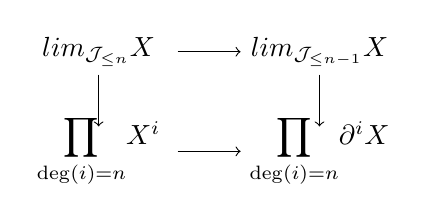
\begin{tikzpicture}[x=1.9em,y=1.5em]
  \node (Ln) at (0,1.3) {${\displaystyle\operatorname{lim}_{\mathcal{J}_{\leq n}}X}$};
  \node (Ln1) at (4.2,1.3) {${\displaystyle\operatorname{lim}_{\mathcal{J}_{\leq n-1}}X}$};
  \node (P1) at (0,-1.1) {${\displaystyle\prod_{\deg(i)=n}}X^i$};
  \node (P2) at (4.2,-1.1) {${\displaystyle\prod_{\deg(i)=n}}\partial^i X$};
  \draw[->] (1.5,1.3) -- (2.7,1.3);
  \node at (1.55,1.0) {$\scriptstyle\lrcorner$};
  \draw[->] (0,0.75) -- (0,-0.5);
  \draw[->] (4.2,0.75) -- (4.2,-0.5);
  \draw[->] (1.5,-1.1) -- (2.7,-1.1);
\end{tikzpicture}
\end{center}
特别地，\trLimit{}\trCone{} $\operatorname{lim}_{\mathcal{J}}X\to X^i$
的每条腿都是\trFibration，纤维性图表 $X$ 的像中的每个映射亦然。
\item 对纤维性图表之间的任何纤维性自然变换
  $\alpha\colon X\to Y\in\mathcal{M}^{\mathcal{J}}$，诱导映射
  $\operatorname{lim}_{\mathcal{J}}X\to\operatorname{lim}_{\mathcal{J}}Y$
  是一座塔的极限复合，其第 $n$ 层是映射 $p_n$ 的一个\trPullback，该映射
  构造为下图中的拉回：
\begin{rveq}\label{eq:tower-cube}
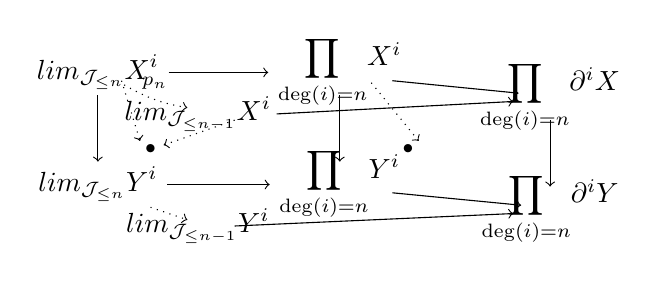
\begin{tikzpicture}[x=1.9em,y=1.5em]
  \node (An) at (0,2.6) {${\displaystyle\operatorname{lim}_{\mathcal{J}_{\leq n}}X^i}$};
  \node (Bn) at (4.6,2.6) {${\displaystyle\prod_{\deg(i)=n}}X^i$};
  \node (Cn) at (8.6,2.0) {${\displaystyle\prod_{\deg(i)=n}}\partial^i X$};
  \node (An1) at (1.9,1.6) {${\displaystyle\operatorname{lim}_{\mathcal{J}_{\leq n-1}}X^i}$};
  \node (d1) at (1.0,0.75) {$\scriptstyle\bullet$};
  \node (d2) at (5.9,0.75) {$\scriptstyle\bullet$};
  \node (F) at (0,-0.1) {${\displaystyle\operatorname{lim}_{\mathcal{J}_{\leq n}}Y^i}$};
  \node (G) at (4.6,-0.1) {${\displaystyle\prod_{\deg(i)=n}}Y^i$};
  \node (H) at (8.6,-0.7) {${\displaystyle\prod_{\deg(i)=n}}\partial^i Y$};
  \node (I) at (1.9,-1.1) {${\displaystyle\operatorname{lim}_{\mathcal{J}_{\leq n-1}}Y^i}$};
  \draw[->] (An) -- (Bn);
  \draw[->] (5.6,2.4) -- (8.0,2.1);
  \draw[dotted,->] (0.5,2.3) to[bend right=10] node[pos=0.5,above]{$\scriptstyle p_n$} (1.7,1.75);
  \draw[dotted,->] (0.45,2.4) -- (0.8,0.95);
  \draw[dotted,->] (2.6,1.45) -- (1.25,0.85);
  \draw[dotted,->] (5.2,2.35) -- (6.1,0.95);
  \draw[->] (3.4,1.6) -- (7.9,1.9);
  \node at (1.28,0.55) {$\scriptstyle\lrcorner$};
  \node at (6.18,0.55) {$\scriptstyle\lrcorner$};
  \draw[->] (0,2.05) -- (0,0.45);
  \draw[->] (4.6,2.05) -- (4.6,0.45);
  \draw[->] (8.6,1.45) -- (8.6,-0.15);
  \draw[->] (2.6,-1.1) -- (7.9,-0.8);
  \draw[->] (F) -- (G);
  \draw[->] (5.6,-0.3) -- (8.05,-0.6);
  \draw[dotted,->] (1.0,-0.65) -- (1.7,-0.95);
\end{tikzpicture}
\end{rveq}
此外，每个分量映射 $\alpha^i\colon X^i\rvFarrow Y^i$ 都是\trFibration。
\end{enumerate}
\end{proposition}

\begin{proof}
注意切片\trCategory{} $i\backslash\mathcal{J}_{n-1}$ 仍是一个逆范畴，其度\trFunctor{}为
\[
i\backslash\mathcal{J}_{n-1}\xrightarrow{\ \mathrm{cod}\ }\mathcal{J}_{n-1}
\xrightarrow{\ \deg\ }\omega^{\mathrm{op}}
\]
其中每个对象的度数至多为 $n-1$。在 $i$ 的度数为 $1$ 的情形，该\trCategory{}%
只有恒同箭头，于是由归纳法我们可以假定\eqref{eq:boundary-object} 所定义的
$\partial^i X$ 存在。现在，(i) 的结果由直接检视这一构造的\trUniversalProperty{}%
而得出，一如\cref{prop:tower-limits} 之证明中的做法。最后的论断由这一构造
随之而来，其验证留给\cref{ex:component-fibrations}。

由 (i) 可知，诸逆向极限之间的诱导映射定义为\trCategoryOfArrows{}
$\mathcal{M}^{\mathbf{2}}$ 中一个 $\omega^{\mathrm{op}}$ 标引\trDiagram{}的%
\trLimit{}：
\begin{center}
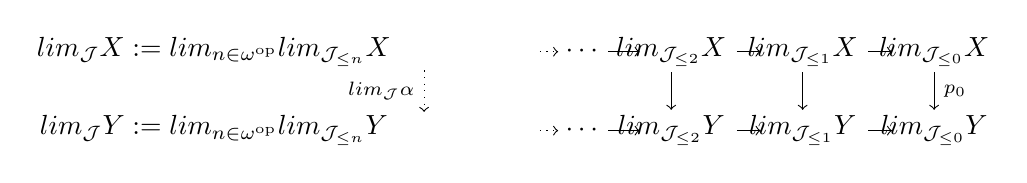
\begin{tikzpicture}[x=1.9em,y=1.5em]
  \node (Xt) at (0,1.3) {$\operatorname{lim}_{\mathcal{J}}X:=\operatorname{lim}_{n\in\omega^{\mathrm{op}}}\operatorname{lim}_{\mathcal{J}_{\leq n}}X$};
  \node (Xd) at (7.0,1.3) {$\cdots$};
  \node (X2) at (8.7,1.3) {$\operatorname{lim}_{\mathcal{J}_{\leq 2}}X$};
  \node (X1) at (11.2,1.3) {$\operatorname{lim}_{\mathcal{J}_{\leq 1}}X$};
  \node (X0) at (13.7,1.3) {$\operatorname{lim}_{\mathcal{J}_{\leq 0}}X$};
  \node (Yt) at (0,-0.6) {$\operatorname{lim}_{\mathcal{J}}Y:=\operatorname{lim}_{n\in\omega^{\mathrm{op}}}\operatorname{lim}_{\mathcal{J}_{\leq n}}Y$};
  \node (Yd) at (7.0,-0.6) {$\cdots$};
  \node (Y2) at (8.7,-0.6) {$\operatorname{lim}_{\mathcal{J}_{\leq 2}}Y$};
  \node (Y1) at (11.2,-0.6) {$\operatorname{lim}_{\mathcal{J}_{\leq 1}}Y$};
  \node (Y0) at (13.7,-0.6) {$\operatorname{lim}_{\mathcal{J}_{\leq 0}}Y$};
  \draw[dotted,->] (6.2,1.3) -- (6.55,1.3);
  \draw[->] (7.5,1.3) -- (8.1,1.3);
  \draw[->] (9.95,1.3) -- (10.4,1.3);
  \draw[->] (12.45,1.3) -- (12.9,1.3);
  \draw[dotted,->] (6.2,-0.6) -- (6.55,-0.6);
  \draw[->] (7.5,-0.6) -- (8.1,-0.6);
  \draw[->] (9.95,-0.6) -- (10.4,-0.6);
  \draw[->] (12.45,-0.6) -- (12.9,-0.6);
  \draw[dotted,->] (4.0,0.85) -- (4.0,-0.15) node[midway,left]{$\scriptstyle\operatorname{lim}_{\mathcal{J}}\alpha$};
  \draw[->] (8.7,0.8) -- (8.7,-0.1);
  \draw[->] (11.2,0.8) -- (11.2,-0.1);
  \draw[->] (13.7,0.8) -- (13.7,-0.1) node[midway,right]{$\scriptstyle p_0$};
\end{tikzpicture}
\end{center}
在 (ii) 的假设下，由\cref{prop:tower-limits}(i) 的证明可得：映射
$\operatorname{lim}_{\mathcal{J}}\alpha$ 随之分解为一座塔的极限复合，其
底层是映射 $p_0$ 沿上方较低水平复合的\trPullback，其下一层是出现于最右侧
方块中的映射 $p_1$ 的\trPullback，再下一层是出现于第二右侧方块中的映射
$p_2$ 的\trPullback，依此类推，其中在每个方块中，$p_n$ 都是从左上角到
右下余跨度之\trPullback{}的映射。映射 $p_0$ 是以度数为零的对象为标的诸
相对匹配映射之积，因而是一个\trFibration。在立方体 \eqref{eq:tower-cube}
中应用\trPullback{}的复合与消去可知：由 (i)，顶面与底面都是拉回方块，于是映射
$p_n$——从初始顶点到左面中的拉回——是从
$\prod_{\deg(i)=n}X^i$ 到右面中拉回的对应映射的一个\trPullback。这一映射是
以度数为 $n$ 的对象为标的诸相对匹配映射之积，从而是一个\trFibration，故
$p_n$ 也是一个\trFibration。于是，由\cref{prop:tower-limits}(i)，诱导映射
$\operatorname{lim}_{\mathcal{J}}\alpha\colon\operatorname{lim}_{\mathcal{J}}X\to\operatorname{lim}_{\mathcal{J}}Y$
也是一个\trFibration。这就证明了 (ii) 中除最后一个断言之外的全部内容，
而后者同样留给\cref{ex:component-fibrations}。
\end{proof}

我们还想进一步断言：对以逆范畴为标引的纤维性图表之间的任何%
\trPointwise{}\trWeakEquivalence{} $\alpha\colon X\to Y\in\mathcal{M}^{\mathcal{J}}$，
诱导映射 $\operatorname{lim}_{\mathcal{J}}X\to\operatorname{lim}_{\mathcal{J}}Y$
是一个\trWeakEquivalence。一如\cref{prop:tower-limits}(ii) 的证明，这需要
一个具有独立兴趣的中间结果，它与练习 6.1.iii 密切相关。

\begin{proposition}\label{prop:fibrant-diagram-cfo}
设 $\mathcal{M}$ 是一个配有\trFibration{}类 $\rvF$ 与\trWeakEquivalence{}%
类 $\rvW$ 的\trCategoryOfFibrantObjects，并设 $\mathcal{J}$ 是一个逆范畴。由纤维性图表
与其间的全部\trNaturalTransformation{}构成的\trCategory{}
$\mathcal{M}^{\mathcal{J}}$ 继承一个\trCategoryOfFibrantObjects{}的结构，其中：
\begin{itemize}
\item 诸\trWeakEquivalence{}是诸分量居于 $\rvW$ 中的那些%
  \trNaturalTransformation{}；
\item 诸\trFibration{}是诸纤维性自然变换，即那些
  $\alpha\colon X\to Y\in\mathcal{M}^{\mathcal{J}}$，使得对每个
  $i\in\mathcal{J}$，相对匹配映射
  $X^i\xrightarrow{\ \hat{m}^i\ \rvFarrow\ }Y^i\times_{\partial^i Y}\partial^i X$
  属于 $\rvF$；
\item 诸\trTrivialFibration{}是那些
  $\alpha\colon X\to Y\in\mathcal{M}^{\mathcal{J}}$，使得对每个
  $i\in\mathcal{J}$，相对匹配映射
  $X^i\xrightarrow{\ \hat{m}^i\ \rvTFarrow\ }Y^i\times_{\partial^i Y}\partial^i X$
  属于 $\rvF\cap\rvW$。
\end{itemize}
\end{proposition}

\begin{proof}
这一证明对读者而言是一项颇为冗长的练习，它只是把 C.4 节中的相应论证特化到
这一「单边」情形。使用一个略有不同的公理化的类似结果的证明，可见
\cite[9.2.4]{bib94}。
\end{proof}

这一切工作的回报是如下结果。

\begin{proposition}\label{prop:inverse-limits-we}
设 $\mathcal{M}$ 是一个\trCategoryOfFibrantObjects，并设 $\mathcal{J}$ 是一个逆范畴。
那么，对纤维性图表之间的任何\trPointwise{}\trWeakEquivalence{}
$\alpha\colon X\to Y\in\mathcal{M}^{\mathcal{J}}$，诸\trLimit{}之间的诱导
映射 $\operatorname{lim}_{\mathcal{J}}X\to\operatorname{lim}_{\mathcal{J}}Y$
是一个\trWeakEquivalence。
\end{proposition}

\begin{proof}
我们利用\cref{prop:fibrant-diagram-cfo}，它赋予纤维性图表的\trCategory{}
$\mathcal{M}^{\mathcal{J}}$ 以\trCategoryOfFibrantObjects{}的结构。考虑 $\rvF$ 中或
$\rvF\cap\rvW$ 中的一个映射 $\alpha\colon X\to Y\in\mathcal{M}^{\mathcal{J}}$。
由\cref{prop:general-towers}(ii)，这一映射是一座映射塔的极限复合，其每一层
都是我们已假设居于 $\rvF$ 或 $\rvF\cap\rvW$ 中的那些映射之积的一个%
\trPullback。由于类 $\rvF$ 与 $\rvF\cap\rvW$ 对\trProduct、\trPullback{}与
塔的\trLimit{}封闭，现在已然清楚：\trLimit{}\trFunctor{}保持这些类。而它也
保持类 $\rvW$ 这一事实，则由\cref{lem:ken-brown} 得出。
\end{proof}

\begin{exercise}\label{ex:cospan-cfo}
证明：对任何\trCategoryOfFibrantObjects{} $\mathcal{M}$，都存在一个%
\trCategoryOfFibrantObjects{} $\mathcal{M}^{\perp}$，其
\begin{itemize}
\item 对象是\trCospan{} $C\xrightarrow{g}A\xleftarrow{f}B$，其中右腿是
  $\mathcal{M}$ 中的一支\trFibration；
\item \trWeakEquivalence{}是\trPointwise{}\trWeakEquivalence；并且
\item \trFibration{}是形如下图的\trDiagram，其中映射 $r$、$p$ 与 $q$ 都是%
  \trFibration，而诱导映射 $z\colon B\to A\times_{\bar{A}}\bar{B}$ 亦然：
\begin{center}
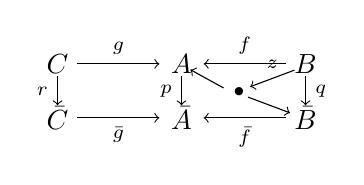
\begin{tikzpicture}[x=1.6em,y=1.5em]
  \node (C) at (0,1.3) {$C$};
  \node (A) at (2.8,1.3) {$A$};
  \node (B) at (5.6,1.3) {$B$};
  \node (Cb) at (0,0) {$\bar{C}$};
  \node (Ab) at (2.8,0) {$\bar{A}$};
  \node (Bb) at (5.6,0) {$\bar{B}$};
  \node (dot) at (4.1,0.62) {$\scriptstyle\bullet$};
  \draw[->] (0.45,1.3) -- (2.3,1.3) node[midway,above]{$\scriptstyle g$};
  \draw[->] (5.15,1.3) -- (3.3,1.3) node[midway,above]{$\scriptstyle f$};
  \draw[->] (0,1.0) -- (0,0.3) node[midway,left]{$\scriptstyle r$};
  \draw[->] (2.8,1.0) -- (2.8,0.3) node[midway,left]{$\scriptstyle p$};
  \draw[->] (5.6,1.0) -- (5.6,0.3) node[midway,right]{$\scriptstyle q$};
  \draw[->] (0.45,0) -- (2.3,0) node[midway,below]{$\scriptstyle\bar{g}$};
  \draw[->] (5.15,0) -- (3.3,0) node[midway,below]{$\scriptstyle\bar{f}$};
  \draw[->] (5.35,1.15) -- (4.35,0.75) node[pos=0.5,above]{$\scriptstyle z$};
  \draw[->] (3.75,0.72) -- (3.0,1.16);
  \draw[->] (4.3,0.5) -- (5.25,0.12);
  \node at (4.42,0.5) {$\scriptstyle\lrcorner$};
\end{tikzpicture}
\end{center}
\end{itemize}
而所需的诸\trLimit{}则逐点继承自 $\mathcal{M}$。
\end{exercise}

\begin{exercise}\label{ex:towers-cfo}
将\cref{prop:fibrant-diagram-cfo} 特化，以描述\trCategoryOfFibrantObjects{} $\mathcal{M}$
中诸\trFibration{}塔的\trCategory{} $\mathcal{M}^{\omega^{\mathrm{op}}}$
上的\trCategoryOfFibrantObjects{}结构，并以之为\cref{prop:tower-limits}(ii) 的证明补全
收官。
\end{exercise}

\begin{exercise}\label{ex:component-fibrations}
\cref{prop:reedy-components}
\begin{enumerate}[label=(\roman*)]
\item 验证\cref{prop:general-towers}(i) 中所构造的\trLimit{}\trCone{}的
  每条腿都是一个\trFibration。
\item 由此推论：纤维性图表的像中的每个态射都是一个\trFibration。
\item 沿同样的路线论证，验证纤维性自然变换的每个分量都是一个%
  \trFibration。
\end{enumerate}
\end{exercise}

\begin{exercise}\label{ex:prove-c123}
证明\cref{prop:fibrant-diagram-cfo}，并判定\cref{ex:cospan-cfo} 与%
\cref{ex:towers-cfo} 是否为这一结果的特例。
\end{exercise}
   %

\providecommand{\llsq}{\mathrel{\square}}%

\section{提升性质、弱分解系统与 Leibniz 闭性}\label{sec:weak-factorization-systems}

固定\trCategory{} $\mathcal{M}$ 中的两个箭头 $j$ 与 $p$，我们把任何形如
\begin{center}
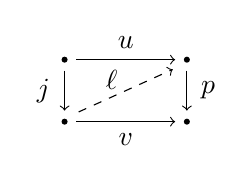
\begin{tikzpicture}[x=1.7em,y=1.6em]
  \fill (0,1.4) circle (1.1pt);
  \fill (2.6,1.4) circle (1.1pt);
  \fill (0,0) circle (1.1pt);
  \fill (2.6,0) circle (1.1pt);
  \draw[->] (0.25,1.4) -- (2.35,1.4);
  \node at (1.3,1.78) {$u$};
  \draw[->] (0,1.15) -- (0,0.25);
  \node at (-0.45,0.7) {$j$};
  \draw[->] (2.6,1.15) -- (2.6,0.25);
  \node at (3.05,0.7) {$p$};
  \draw[->] (0.25,0) -- (2.35,0);
  \node at (1.3,-0.4) {$v$};
  \draw[->,dashed] (0.3,0.22) -- (2.3,1.18);
  \node at (1.0,0.95) {$\ell$};
\end{tikzpicture}
\end{center}
的交换方块视作 $j$ 与 $p$ 之间的一个\trLifting{}问题，它经由构造一个提升——
一条使两个三角形都交换的对角态射 $\ell$——而得解。若 $j$ 与 $p$ 之间的每个%
\trLifting{}问题都有解，我们便说 $j$ 对 $p$ 具有\textbf{左\trLifting{}性质}%
（left lifting property），等价地，$p$ 对 $j$ 具有\textbf{右%
\trLifting{}性质}（right lifting property）。此时，我们采用富有暗示意味的
记号 $j\llsq p$ 来断言这一提升性质。

在抽象\trHomotopy{}论中，令人感兴趣的映射类时常由对另一类或一集映射的左或
右\trLifting{}性质来刻画。

\begin{definition}\label{def:lifting-classes}
设 $J$ 是\trCategory{} $\mathcal{M}$ 中的一个映射类。
\begin{itemize}
\item 记 $J\llsq$ 为 $\mathcal{M}$ 中对 $J$ 中每个态射都具有右\trLifting{}性质
  的映射组成的类。
\item 记 $\llsq J$ 为 $\mathcal{M}$ 中对 $J$ 中每个态射都具有左\trLifting{}性质
  的映射组成的类。
\end{itemize}
\end{definition}

\begin{example}\label{exa:isofibration-trivial-lifting}
第 1 章中的\cref{def:isofibration}与\cref{def:trivial-fibration}以对映射之集
\[ \{\Lambda^k[n]\hookrightarrow\Delta[n]\}_{n\ge 2,\,0<k<n}
   \cup\{\qcOne\hookrightarrow\qcInt\}
   \qquad\text{与}\qquad
   \{\partial\Delta[n]\hookrightarrow\Delta[n]\}_{n\ge 0} \]
的右\trLifting{}性质，分别刻画了\trQuasiCategory{}之间的\trIsofibration{}与%
\trTrivialFibration。
\end{example}

由右\trLifting{}性质刻画的映射自动满足各种如今或许已经眼熟的封闭性质。

\begin{lemma}\label{lem:right-lifting-closure}
由右\trLifting{}性质刻画的任何映射类 $J\llsq$ 都包含全部\trIsomorphism，并对
复合、\trProduct、\trPullback、\trRetract{}以及塔的\trLimit{}封闭。
\end{lemma}

在陈述中，「积」与「收缩」指称在\trCategoryOfArrows{}中构成的极限，而「拉回」
则是 $J\llsq$ 中的映射沿任一映射的拉回。「塔」指形状为 $\alpha^{\mathrm{op}}$ 的
图表，其中 $\alpha$ 是一个极限序数（极可能是 $\omega$）。

\begin{proof}
诸论证皆类似。例如，设 $q$ 是 $p\in J\llsq$ 的一个\trPullback。把下方左侧的%
\trLifting{}问题与下方右侧的\trPullback{}方块并置，便可求解 $j$ 对 $p$ 的复合%
\trLifting{}问题而得到虚对角态射 $\ell$，然后经由在\trPullback{}图式上由
$(v,\ell)$ 构成的\trCone，诱导出 $j$ 对 $q$ 的\trLifting{}问题的一个解 $s$：
\begin{center}
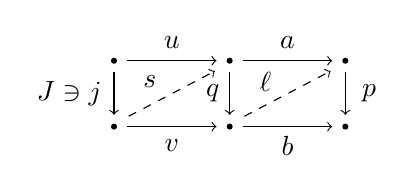
\begin{tikzpicture}[x=1.9em,y=1.7em]
  \fill (0,1.4) circle (1.1pt);
  \fill (2.2,1.4) circle (1.1pt);
  \fill (4.4,1.4) circle (1.1pt);
  \fill (0,0) circle (1.1pt);
  \fill (2.2,0) circle (1.1pt);
  \fill (4.4,0) circle (1.1pt);
  \draw[->] (0.25,1.4) -- (1.95,1.4);
  \node at (1.1,1.78) {$u$};
  \draw[->] (2.45,1.4) -- (4.15,1.4);
  \node at (3.3,1.78) {$a$};
  \draw[->] (0,1.15) -- (0,0.25);
  \node at (-0.85,0.7) {$J\owns j$};
  \draw[->] (2.2,1.15) -- (2.2,0.25);
  \node at (1.88,0.7) {$q$};
  \draw[->] (4.4,1.15) -- (4.4,0.25);
  \node at (4.85,0.7) {$p$};
  \draw[->] (0.25,0) -- (1.95,0);
  \node at (1.1,-0.4) {$v$};
  \draw[->] (2.45,0) -- (4.15,0);
  \node at (3.3,-0.4) {$b$};
  \draw[->,dashed] (0.28,0.22) -- (1.92,1.18);
  \node at (0.68,0.95) {$s$};
  \draw[->,dashed] (2.48,0.22) -- (4.12,1.18);
  \node at (2.88,0.95) {$\ell$};
  \node at (2.55,1.08) {$\scriptstyle\lrcorner$};
\end{tikzpicture}
\end{center}
于是 $q$ 对 $J$ 可提升，从而属于 $J\llsq$。
\end{proof}

由于\cref{lem:right-lifting-closure}的对偶，余完备\trCategory{}中的任何映射之
集都「胞腔式生成」一个更大的、具有同一左\trLifting{}性质的映射类。

\begin{definition}\label{def:cell-complex}
设 $J$ 是一个我们视作「基本\trCell{}」的映射之集。一个%
\textbf{$J$-胞腔复形}（$J$-cell complex）是一个作为 $J$ 中映射之余积的推出经
超限复合而构筑起来的映射：
\begin{center}
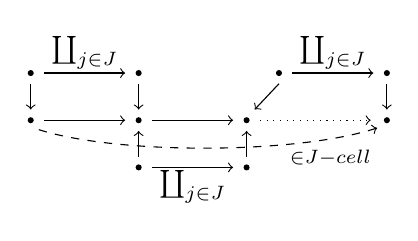
\begin{tikzpicture}[x=1.95em,y=1.55em]
  \fill (0,2.2) circle (1.1pt);
  \fill (2.0,2.2) circle (1.1pt);
  \fill (4.6,2.2) circle (1.1pt);
  \fill (6.6,2.2) circle (1.1pt);
  \fill (0,1.1) circle (1.1pt);
  \fill (2.0,1.1) circle (1.1pt);
  \fill (4.0,1.1) circle (1.1pt);
  \fill (6.6,1.1) circle (1.1pt);
  \fill (2.0,0) circle (1.1pt);
  \fill (4.0,0) circle (1.1pt);
  \draw[->] (0.25,2.2) -- (1.75,2.2);
  \node at (1.0,2.66) {$\coprod_{j\in J}$};
  \draw[->] (4.85,2.2) -- (6.35,2.2);
  \node at (5.6,2.66) {$\coprod_{j\in J}$};
  \draw[->] (0,1.95) -- (0,1.35);
  \draw[->] (2.0,1.95) -- (2.0,1.35);
  \draw[->] (4.6,1.95) -- (4.15,1.35);
  \draw[->] (6.6,1.95) -- (6.6,1.35);
  \draw[->] (0.25,1.1) -- (1.75,1.1);
  \draw[->] (2.25,1.1) -- (3.75,1.1);
  \draw[->,dotted] (4.25,1.1) -- (6.3,1.1);
  \draw[->] (2.0,0.25) -- (2.0,0.85);
  \draw[->] (4.0,0.25) -- (4.0,0.85);
  \draw[->] (2.25,0) -- (3.75,0);
  \node at (3.0,-0.46) {$\coprod_{j\in J}$};
  \node at (1.68,1.4) {$\lrcorner$};
  \node at (4.32,0.82) {$\urcorner$};
  \draw[->,dashed] (0.15,0.88) .. controls (1.6,0.3) and (4.9,0.3) .. (6.42,0.92);
  \node at (5.55,0.22) {$\scriptstyle\in J\text{-cell}$};
\end{tikzpicture}
\end{center}
\end{definition}

诸 $J$-胞腔复形组成的类 $J\text{-cell}$ 称为由映射之集 $J$ \trCell{}式生成。
由映射之集 $J$ \textbf{余纤维性生成}（cofibrantly generated）的映射类
$J\text{-cof}$，由那些作为这些映射之余积的推出的序列复合的收缩而得到的映射
组成。

\begin{definition}\label{def:weak-factorization-system}
\trCategory{} $\mathcal{M}$ 上的一个弱分解系统 $(\mathrm{L},\mathrm{R})$ 由
态射类 $\mathrm{L}$ 与 $\mathrm{R}$ 组成，使得
\begin{enumerate}[label=(\roman*)]
\item $\mathcal{M}$ 中每个态射都可分解为 $\mathrm{L}$ 中一个态射接 $\mathrm{R}$
  中一个态射：
\begin{center}
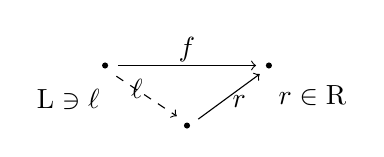
\begin{tikzpicture}[x=1.85em,y=1.55em]
  \fill (0,1.4) circle (1.1pt);
  \fill (3.2,1.4) circle (1.1pt);
  \fill (1.6,0) circle (1.1pt);
  \draw[->] (0.25,1.4) -- (2.95,1.4);
  \node at (1.6,1.78) {$f$};
  \draw[->,dashed] (0.22,1.15) -- (1.4,0.22);
  \node at (-0.72,0.62) {$\mathrm{L}\owns\ell$};
  \node at (0.62,0.85) {$\ell$};
  \draw[->] (1.82,0.15) -- (3.02,1.2);
  \node at (2.62,0.55) {$r$};
  \node at (4.05,0.7) {$r\in\mathrm{R}$};
\end{tikzpicture}
\end{center}
\item 类 $\mathrm{L}$ 与 $\mathrm{R}$ 彼此之间分别具有左、右\trLifting{}性质
  $\mathrm{L}\llsq\mathrm{R}$；也就是说，从 $\mathrm{L}$ 中一个映射到
  $\mathrm{R}$ 中一个映射的任何交换方块都有对角填充：
\begin{center}
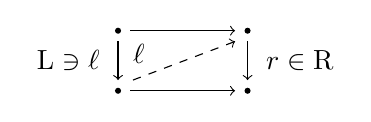
\begin{tikzpicture}[x=1.8em,y=1.55em]
  \fill (0,1.4) circle (1.1pt);
  \fill (2.6,1.4) circle (1.1pt);
  \fill (0,0) circle (1.1pt);
  \fill (2.6,0) circle (1.1pt);
  \draw[->] (0.25,1.4) -- (2.35,1.4);
  \draw[->] (0,1.15) -- (0,0.25);
  \node at (-1.0,0.7) {$\mathrm{L}\owns\ell$};
  \node at (0.42,0.85) {$\ell$};
  \draw[->] (2.6,1.15) -- (2.6,0.25);
  \node at (3.65,0.7) {$r\in\mathrm{R}$};
  \draw[->,dashed] (0.3,0.25) -- (2.35,1.15);
  \draw[->] (0.25,0) -- (2.35,0);
\end{tikzpicture}
\end{center}
\item 并且 $\mathrm{L}=\llsq\mathrm{R}$ 而 $\mathrm{R}=\mathrm{L}\llsq$。
\end{enumerate}
\end{definition}

作为\cref{def:weak-factorization-system}(iii) 的推论，弱分解系统的右类享有
\cref{lem:right-lifting-closure}的诸封闭性质，而左类则对对偶构造封闭。

在一对伴随\trFunctor{}在场时，提升性质可以转置。

\begin{lemma}\label{lem:adjunction-transposes-lifting}
在伴随在场时：
\begin{center}
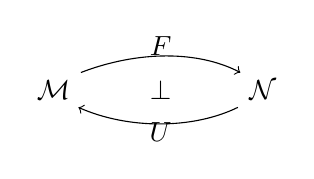
\begin{tikzpicture}[x=1.8em,y=1.5em]
  \node (M) at (0,0) {$\mathcal{M}$};
  \node (N) at (4.2,0) {$\mathcal{N}$};
  \draw[->] (0.55,0.42) .. controls (1.7,0.95) and (2.9,0.95) .. (3.75,0.42);
  \node at (2.15,1.05) {$F$};
  \draw[->] (3.7,-0.42) .. controls (2.8,-0.95) and (1.5,-0.95) .. (0.5,-0.42);
  \node at (2.15,-1.02) {$U$};
  \node at (2.15,0) {$\perp$};
\end{tikzpicture}
\end{center}
\begin{enumerate}[label=(\roman*)]
\item 下方左侧所示的 $\mathcal{N}$ 中\trLifting{}问题的解经转置可定义下方右侧
  所示的 $\mathcal{M}$ 中转置\trLifting{}问题的解：
\begin{center}
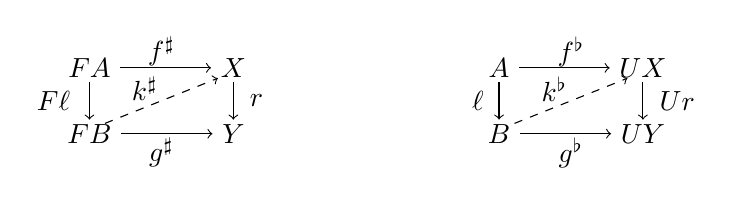
\begin{tikzpicture}[x=2.0em,y=1.7em]
  \node (FA) at (0,1.4) {$FA$};
  \node (X) at (2.6,1.4) {$X$};
  \node (FB) at (0,0) {$FB$};
  \node (Y) at (2.6,0) {$Y$};
  \draw[->] (FA) -- (X);
  \node at (1.3,1.74) {$f^{\sharp}$};
  \draw[->] (0,1.1) -- (0,0.3);
  \node at (-0.65,0.7) {$F\ell$};
  \draw[->] (2.6,1.1) -- (2.6,0.3);
  \node at (3.02,0.7) {$r$};
  \draw[->] (FB) -- (Y);
  \node at (1.3,-0.4) {$g^{\sharp}$};
  \draw[->,dashed] (0.28,0.22) -- (2.32,1.18);
  \node at (1.0,0.95) {$k^{\sharp}$};
  \node (A) at (7.4,1.4) {$A$};
  \node (UX) at (10.0,1.4) {$UX$};
  \node (B) at (7.4,0) {$B$};
  \node (UY) at (10.0,0) {$UY$};
  \draw[->] (A) -- (UX);
  \node at (8.7,1.74) {$f^{\flat}$};
  \draw[->] (7.4,1.1) -- (7.4,0.3);
  \node at (7.02,0.7) {$\ell$};
  \draw[->] (10.0,1.1) -- (10.0,0.3);
  \node at (10.62,0.7) {$Ur$};
  \draw[->] (B) -- (UY);
  \node at (8.7,-0.4) {$g^{\flat}$};
  \draw[->,dashed] (7.68,0.22) -- (9.72,1.18);
  \node at (8.4,0.95) {$k^{\flat}$};
\end{tikzpicture}
\end{center}
\item 若 $\mathcal{M}$ 带有弱分解系统 $(\mathrm{L},\mathrm{R})$ 而
  $\mathcal{N}$ 带有弱分解系统 $(\mathrm{L}',\mathrm{R}')$，则 $F$ 保持左类
  当且仅当 $U$ 保持右类：
  \[ \mathrm{FL}\subset\mathrm{L}'
     \quad\leftrightsquigarrow\quad
     \mathrm{R}\supset U\mathrm{R}'. \]
\end{enumerate}
\end{lemma}

\cref{def:weak-factorization-system}的诸分解式与 (ii) 全然无关，但我们仍针对
弱分解系统陈述这一结果，因为这正是它通常被应用的语境。
\begin{proof}
\cref{ex:prove-adjunction-transposes}。
\end{proof}

\cref{lem:adjunction-transposes-lifting}(ii) 定义了\textbf{弱分解系统的伴随}%
（adjunction of weak factorization systems）这一概念：这是配备弱分解系统的诸%
\trCategory{}之间的一对伴随\trFunctor，使得左\trAdjunction{}保持左类而右%
\trAdjunction{}保持右类。我们现在的目标是把这一概念推广到双变量\trAdjunction{}上，%
\footnote{对 $n$-变量\trAdjunction{}有一个类似的推广，可在 \cite[\S4]{bib26}
中找到。}后者由一个三元组的\trBifunctor{}给出：
\begin{rveq}\label{eq:two-variable-adjunction-functors}
\mathcal{V}\times\mathcal{M}\xrightarrow{\;\otimes\;}\mathcal{N},\qquad
\mathcal{V}^{\mathrm{op}}\times\mathcal{N}\xrightarrow{\;\{,\}\;}\mathcal{M},
\qquad
\mathcal{M}^{\mathrm{op}}\times\mathcal{N}\xrightarrow{\;\mathrm{hom}\;}\mathcal{V}
\end{rveq}
书写时所用的记号暗示着最常见的例子，并配备有一个自然\trIsomorphism
\[ \mathcal{N}(\mathcal{V}\otimes\mathcal{M},\mathcal{N})
   \cong\mathcal{M}(\mathcal{M},\{\mathcal{V},\mathcal{N}\})
   \cong\mathcal{V}(\mathcal{V},\mathrm{hom}(\mathcal{M},\mathcal{N})). \]

\trBifunctor{} $\otimes\colon\mathcal{V}\times\mathcal{M}\to\mathcal{N}$ 的
「推出积」定义了一个\trBifunctor{}
$\widehat{\otimes}\colon\mathcal{V}^{2}\times\mathcal{M}^{2}\to\mathcal{N}^{2}$；
当该\trBifunctor{} $\otimes$ 被称作「张量」时，我们把 $\widehat{\otimes}$ 称作
「\trLeibnizTensor」。「\trLeibnizCotensor」与「Leibniz hom」
\[ \widehat{\{,\}}\colon(\mathcal{V}^{2})^{\mathrm{op}}\times\mathcal{N}^{2}
     \to\mathcal{M}^{2}
   \qquad\text{与}\qquad
   \widehat{\mathrm{hom}}\colon(\mathcal{M}^{2})^{\mathrm{op}}\times\mathcal{N}^{2}
     \to\mathcal{V}^{2} \]
则对偶地定义，分别在 $\mathcal{M}$ 与 $\mathcal{V}$ 中使用拉回。

\begin{definition}[Leibniz 张量与余张量]\label{def:leibniz-tensor-cotensor}
给定取值于带推出\trCategory{}的\trBifunctor{}
$\otimes\colon\mathcal{V}\times\mathcal{M}\to\mathcal{N}$，$\mathcal{V}$ 中映射
$k\colon I\to J$ 与 $\mathcal{M}$ 中映射 $\ell\colon A\to B$ 的%
\trLeibnizTensor{}是 $\mathcal{N}$ 中由下方左侧的推出图式所诱导的映射
$k\widehat{\otimes}\ell$：
\begin{center}
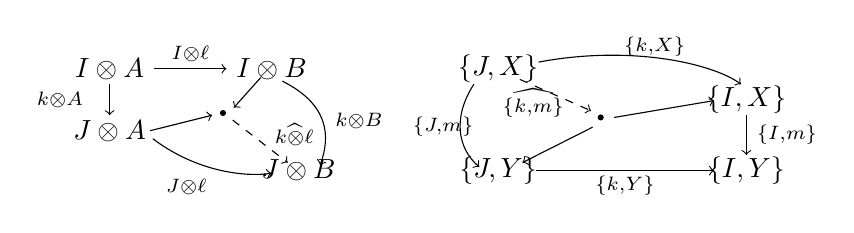
\begin{tikzpicture}[x=1.95em,y=1.6em]
  \node (IA) at (0,1.9) {$I\otimes A$};
  \node (IB) at (3.0,1.9) {$I\otimes B$};
  \node (JA) at (0,0.5) {$J\otimes A$};
  \fill (2.1,0.9) circle (1.1pt);
  \node (JB) at (3.5,-0.4) {$J\otimes B$};
  \draw[->] (IA) -- (IB);
  \node at (1.5,2.24) {$\scriptstyle I\otimes\ell$};
  \draw[->] (0,1.55) -- (0,0.85);
  \node at (-0.92,1.2) {$\scriptstyle k\otimes A$};
  \draw[->] (0.75,0.5) -- (1.9,0.85);
  \draw[->] (2.8,1.7) -- (2.3,1.02);
  \draw[->,dashed] (2.28,0.74) -- (3.3,-0.22);
  \node at (3.42,0.42) {$\scriptstyle k\widehat{\otimes}\ell$};
  \draw[->] (3.2,1.62) .. controls (4.05,1.1) and (4.1,0.4) .. (3.9,-0.28);
  \node at (4.62,0.72) {$\scriptstyle k\otimes B$};
  \draw[->] (0.8,0.32) .. controls (1.6,-0.42) and (2.5,-0.55) .. (3.0,-0.46);
  \node at (1.42,-0.78) {$\scriptstyle J\otimes\ell$};
  \node at (1.82,1.12) {$\lrcorner$};
  \node (JX) at (7.2,1.9) {$\{J,X\}$};
  \node (IX) at (11.8,1.2) {$\{I,X\}$};
  \fill (9.1,0.8) circle (1.1pt);
  \node (JY) at (7.2,-0.4) {$\{J,Y\}$};
  \node (IY) at (11.8,-0.4) {$\{I,Y\}$};
  \draw[->] (7.95,2.05) .. controls (9.7,2.45) and (11.2,2.0) .. (11.7,1.55);
  \node at (10.1,2.4) {$\scriptstyle\{k,X\}$};
  \draw[->] (6.75,1.55) .. controls (6.35,0.8) and (6.45,0.1) .. (6.85,-0.32);
  \node at (6.18,0.6) {$\scriptstyle\{J,m\}$};
  \draw[->] (11.8,0.85) -- (11.8,-0.05);
  \node at (12.55,0.4) {$\scriptstyle\{I,m\}$};
  \draw[->] (7.9,-0.4) -- (11.2,-0.4);
  \node at (9.55,-0.74) {$\scriptstyle\{k,Y\}$};
  \draw[->,dashed] (7.6,1.66) -- (8.92,0.95);
  \node at (7.85,1.12) {$\scriptstyle\widehat{\{k,m\}}$};
  \draw[->] (9.35,0.8) -- (11.2,1.18);
  \draw[->] (8.95,0.58) -- (7.65,-0.22);
  \node at (9.4,1.02) {$\ulcorner$};
\end{tikzpicture}
\end{center}
对于一个变量反变、取值于带拉回\trCategory{}的\trBifunctor{}
$\{,\}\colon\mathcal{V}^{\mathrm{op}}\times\mathcal{N}\to\mathcal{M}$，
$\mathcal{V}$ 中映射 $k\colon I\to J$ 与 $\mathcal{N}$ 中映射 $m\colon X\to Y$
的\trLeibnizCotensor{}是由上方右侧的拉回图式所诱导的映射
$\widehat{\{k,m\}}$。
\end{definition}

\begin{proposition}\label{prop:leibniz-construction-preserves}
Leibniz 构造保持：
\begin{enumerate}[label=(\roman*)]
\item 结构同构：合适可合成的诸\trBifunctor{}之间的一个自然\trIsomorphism
  \[ X\ast(Y\otimes Z)\cong(X\times Y)\mathbin{\square} Z \]
  可扩充为相应\trLeibnizProduct{}之间的一个自然\trIsomorphism
  \[ f\widehat{\ast}\,(g\widehat{\otimes}h)
     \cong(f\widehat{\times}g)\mathbin{\widehat{\square}} h; \]
\item 伴随性：若 $(\otimes,\{,\},\mathrm{hom})$ 定义一个双变量\trAdjunction，
  则诸 Leibniz 函子 $(\widehat{\otimes},\widehat{\{,\}},\widehat{\mathrm{hom}})$
  在相应的\trCategoryOfArrows{}之间定义一个双变量\trAdjunction；
\item 收缩：若 $f$ 是 $h$ 的\trRetract{}而 $g$ 是 $k$ 的\trRetract，则
  $f\widehat{\otimes}g$ 是 $h\widehat{\otimes}k$ 的\trRetract；
\item \trCategoryOfArrows{}中的\trColimit：若
  $\otimes\colon\mathcal{V}\times\mathcal{M}\to\mathcal{N}$ 在任一变量中余连续，
  则 $\widehat{\otimes}\colon\mathcal{V}^{2}\times\mathcal{M}^{2}\to\mathcal{N}^{2}$ 亦然；
\item 推出：若 $\otimes\colon\mathcal{V}\times\mathcal{M}\to\mathcal{N}$ 在其
  第二个变量中余连续，且 $g'$ 是 $g$ 的一个推出，则 $f\widehat{\otimes}g'$ 是
  $f\widehat{\otimes}g$ 的一个推出；
\item 某种意义下的复合：\trLeibnizTensor{} $f\widehat{\otimes}(h\cdot g)$ 可
  分解为 $f\widehat{\otimes}g$ 的一个推出接 $f\widehat{\otimes}h$ 而得的复合
\begin{center}
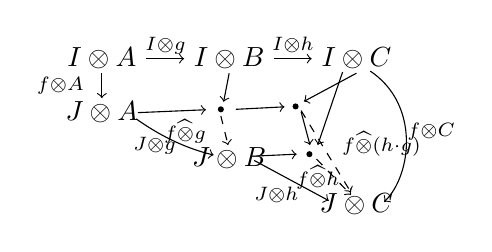
\begin{tikzpicture}[x=2.0em,y=1.5em]
  \node (IA) at (0,2.5) {$I\otimes A$};
  \node (IB) at (2.3,2.5) {$I\otimes B$};
  \node (IC) at (4.6,2.5) {$I\otimes C$};
  \node (JA) at (0,1.2) {$J\otimes A$};
  \fill (2.15,1.28) circle (1.1pt);
  \fill (3.5,1.35) circle (1.1pt);
  \node (JB) at (2.3,0.1) {$J\otimes B$};
  \fill (3.75,0.2) circle (1.1pt);
  \node (JC) at (4.6,-1.0) {$J\otimes C$};
  \draw[->] (IA) -- (IB);
  \node at (1.15,2.82) {$\scriptstyle I\otimes g$};
  \draw[->] (IB) -- (IC);
  \node at (3.45,2.82) {$\scriptstyle I\otimes h$};
  \draw[->] (0,2.15) -- (0,1.55);
  \node at (-0.75,1.85) {$\scriptstyle f\otimes A$};
  \draw[->] (0.65,1.2) -- (1.88,1.27);
  \draw[->] (2.3,2.15) -- (2.2,1.46);
  \draw[->] (4.6,2.15) -- (3.65,1.47);
  \draw[->] (2.42,1.28) -- (3.3,1.34);
  \draw[->,dashed] (2.15,1.12) -- (2.28,0.42);
  \node at (1.5,0.75) {$\scriptstyle f\widehat{\otimes}g$};
  \draw[->] (0.62,1.05) .. controls (1.2,0.5) and (1.7,0.28) .. (2.02,0.18);
  \node at (0.95,0.4) {$\scriptstyle J\otimes g$};
  \draw[->] (2.72,0.15) -- (3.52,0.2);
  \draw[->] (3.6,1.22) -- (3.76,0.42);
  \draw[->] (4.35,2.18) -- (3.9,0.42);
  \draw[->,dashed] (3.6,1.25) -- (4.5,-0.72);
  \node at (5.05,0.45) {$\scriptstyle f\widehat{\otimes}(h\cdot g)$};
  \draw[->,dashed] (3.88,0.08) -- (4.5,-0.78);
  \node at (3.9,-0.35) {$\scriptstyle f\widehat{\otimes}h$};
  \draw[->] (2.75,0.05) -- (4.1,-0.92);
  \node at (3.15,-0.78) {$\scriptstyle J\otimes h$};
  \draw[->] (4.85,2.2) .. controls (5.75,1.4) and (5.6,-0.3) .. (5.1,-0.95);
  \node at (5.95,0.75) {$\scriptstyle f\otimes C$};
  \node at (2.34,1.06) {$\lrcorner$};
  \node at (3.32,1.14) {$\lrcorner$};
  \node at (3.94,0.44) {$\lrcorner$};
\end{tikzpicture}
\end{center}
\item 胞腔复形结构：若 $f$ 与 $g$ 可分别表示为以 $f_{\alpha}$ 与 $g_{\beta}$ 为%
  \trCell{}的胞腔复形，且 $\otimes$ 在两个变量中都余连续，则 $f\widehat{\otimes}g$
  可表示为以 $f_{\alpha}\widehat{\otimes}g_{\beta}$ 为\trCell{}的胞腔复形。
\end{enumerate}
\end{proposition}

\begin{proof}
诸\trLeibnizProduct{}之间诱导结构同构的各分量皆是给定结构同构的实例，因而可逆，这
证明了 (i)。对于 (ii)，由定义双变量\trAdjunction{}
$(\otimes,\{,\},\mathrm{hom})$ 的诸\trIsomorphism{}之自然性，下方三个方块中
每一个可交换当且仅当另外两个可交换，其假设是在两幅图中取相同名称的水平箭头
互为转置：
\begin{center}
\begin{tikzpicture}[x=2.0em,y=1.75em]
  \node (P) at (0.9,1.4) {$J\otimes A\underset{I\otimes A}{\sqcup}I\otimes B$};
  \node (X) at (5.3,1.4) {$X$};
  \node (JB) at (0,0) {$J\otimes B$};
  \node (Y) at (5.3,0) {$Y$};
  \draw[->] (P) -- (X);
  \node at (3.1,1.76) {$\langle u,v\rangle$};
  \draw[->] (0,1.05) -- (0,0.35);
  \node at (-1.05,0.7) {$k\widehat{\otimes}\ell$};
  \draw[->] (5.3,1.05) -- (5.3,0.35);
  \node at (5.68,0.7) {$m$};
  \draw[->] (JB) -- (Y);
  \node at (2.65,-0.4) {$w$};
  \draw[->,dashed] (0.35,0.22) -- (5.0,1.18);
  \node at (1.8,0.9) {$x$};
  \node (A) at (8.0,1.4) {$A$};
  \node (JX) at (11.0,1.4) {$\{J,X\}$};
  \node (B) at (8.0,0) {$B$};
  \node (PB) at (11.6,0) {$\{J,Y\}\underset{\{I,Y\}}{\times}\{I,X\}$};
  \draw[->] (A) -- (JX);
  \node at (9.5,1.76) {$u$};
  \draw[->] (8.0,1.05) -- (8.0,0.35);
  \node at (7.63,0.7) {$\ell$};
  \draw[->] (11.15,1.05) -- (11.5,0.42);
  \node at (12.45,0.78) {$\widehat{\{k,m\}}$};
  \draw[->] (B) -- (PB);
  \node at (9.8,-0.44) {$\langle w,v\rangle$};
  \draw[->,dashed] (8.3,0.22) -- (10.85,1.2);
  \node at (9.4,0.95) {$x$};
\end{tikzpicture}
\end{center}
\begin{center}
\begin{tikzpicture}[x=2.1em,y=1.75em]
  \node (I) at (0,1.4) {$I$};
  \node (hBX) at (4.2,1.4) {$\mathrm{hom}(B,X)$};
  \node (J) at (0,0) {$J$};
  \node (PB) at (5.4,0) {$\mathrm{hom}(A,X)\underset{\mathrm{hom}(A,Y)}{\times}\mathrm{hom}(B,Y)$};
  \draw[->] (I) -- (hBX);
  \node at (2.1,1.76) {$v$};
  \draw[->] (0,1.05) -- (0,0.35);
  \node at (-0.42,0.7) {$k$};
  \draw[->] (4.75,1.1) -- (5.15,0.45);
  \node at (6.0,0.8) {$\widehat{\mathrm{hom}}(\ell,m)$};
  \draw[->] (J) -- (PB);
  \node at (2.35,-0.44) {$\langle u,w\rangle$};
  \draw[->,dashed] (0.35,0.22) -- (4.05,1.22);
  \node at (1.6,0.92) {$x$};
\end{tikzpicture}
\end{center}
这一转置对应可延伸到由这些方块所呈现的\trLifting{}问题的解上
（见\cref{ex:leibniz-lifting-equivalences}）。

性质 (iii) 是 $\widehat{\otimes}$ 在箭头\trCategory{}中的\trBifunctor{}性的
推论：任何\trBifunctor{}都保持收缩。性质 (iv) 几乎同样立即可得，因为%
\trCategoryOfArrows{}中的\trLimit{}与\trColimit{}皆按\trPointwise{}方式计算。
对于 (v)，考虑交换立方：
\begin{center}
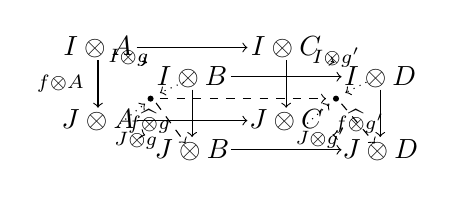
\begin{tikzpicture}[x=2.0em,y=1.32em]
  \node (IA) at (0,2.9) {$I\otimes A$};
  \node (IC) at (3.4,2.9) {$I\otimes C$};
  \node (IB) at (1.7,2.1) {$I\otimes B$};
  \node (ID) at (5.1,2.1) {$I\otimes D$};
  \node (JA) at (0,0.9) {$J\otimes A$};
  \node (JC) at (3.4,0.9) {$J\otimes C$};
  \node (JB) at (1.7,0.1) {$J\otimes B$};
  \node (JD) at (5.1,0.1) {$J\otimes D$};
  \fill (0.95,1.5) circle (1.1pt);
  \fill (4.3,1.5) circle (1.1pt);
  \draw[->] (IA) -- (IB);
  \node at (0.55,2.62) {$\scriptstyle I\otimes g$};
  \draw[->] (IC) -- (ID);
  \node at (4.3,2.62) {$\scriptstyle I\otimes g'$};
  \draw[->] (0.7,2.9) -- (2.7,2.9);
  \draw[->] (2.4,2.1) -- (4.4,2.1);
  \draw[->] (0,2.55) -- (0,1.25);
  \node at (-0.68,1.9) {$\scriptstyle f\otimes A$};
  \draw[->] (JA) -- (JB);
  \node at (0.68,0.36) {$\scriptstyle J\otimes g$};
  \draw[->] (0.7,0.9) -- (2.7,0.9);
  \draw[->] (2.4,0.1) -- (4.4,0.1);
  \draw[->] (1.7,1.75) -- (1.7,0.45);
  \draw[->] (3.4,2.55) -- (3.4,1.25);
  \draw[->] (5.1,1.75) -- (5.1,0.45);
  \draw[->] (JC) -- (JD);
  \node at (4.02,0.42) {$\scriptstyle J\otimes g'$};
  \draw[->,dotted] (1.55,1.95) -- (1.12,1.66);
  \draw[->,dotted] (0.4,0.82) -- (0.85,1.36);
  \draw[->,dashed] (1.05,1.38) -- (1.58,0.28);
  \node at (0.92,0.88) {$\scriptstyle f\widehat{\otimes}g$};
  \draw[->,dotted] (4.85,1.95) -- (4.47,1.66);
  \draw[->,dotted] (3.78,0.82) -- (4.18,1.36);
  \draw[->,dashed] (4.4,1.36) -- (5.0,0.28);
  \node at (4.72,0.88) {$\scriptstyle f\widehat{\otimes}g'$};
  \draw[->,dashed] (1.12,1.5) -- (4.12,1.5);
  \node at (1.18,1.64) {$\lrcorner$};
  \node at (4.52,1.64) {$\lrcorner$};
\end{tikzpicture}
\end{center}
由于 $I\otimes-$ 与 $J\otimes-$ 保持把 $g'$ 定义为 $g$ 之推出的那个推出，
立方的顶面与底面都是推出。定义诸\trLeibnizTensor{}之定义域的那些方块则在
左手面与右手面内部定义了推出。于是由推出的复合与消去即得所断言者：
$f\widehat{\otimes}g'$ 是 $f\widehat{\otimes}g$ 的一个推出。

(vi) 中展示的图式证明了那里所作的断言，故只剩下 (vii) 待证。首先注意：推出
的超限复合的推出仍是推出的超限复合，而超限复合的超限复合仍是超限复合，因此
只需逐个变量地工作，证明 $f\widehat{\otimes}-$ 保持 $g$ 的胞腔复形表示。为此，
设 $g$ 是诸映射 $g_i$ 的一个 $\alpha$-复合，其中每一个都是映射之余积
$g'_i=\coprod_{J}g'_{i,j}$ 的推出。我们可以把这个余极限提升到\trCategoryOfArrows{}%
中，将 $g=g_{0,\alpha}$ 视作\trDiagram{}
$g_{-,\alpha}\colon\alpha\to\mathcal{M}^{2}$ 的余极限，其单步映射为
\begin{center}
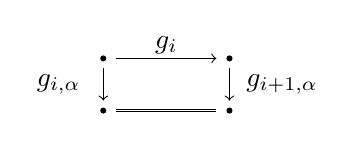
\begin{tikzpicture}[x=1.9em,y=1.45em]
  \fill (0,1.3) circle (1.1pt);
  \fill (2.4,1.3) circle (1.1pt);
  \fill (0,0) circle (1.1pt);
  \fill (2.4,0) circle (1.1pt);
  \draw[->] (0.25,1.3) -- (2.15,1.3);
  \node at (1.2,1.62) {$g_i$};
  \draw[->] (0,1.05) -- (0,0.25);
  \node at (-0.85,0.65) {$g_{i,\alpha}$};
  \draw[->] (2.4,1.05) -- (2.4,0.25);
  \node at (3.4,0.65) {$g_{i+1,\alpha}$};
  \draw[double] (0.25,0) -- (2.15,0);
\end{tikzpicture}
\end{center}

类似地，由 $g'_i$ 定义 $g_i$ 的那个推出方块可以提升为\trCategoryOfArrows{}中的
一个推出方块：
\begin{center}
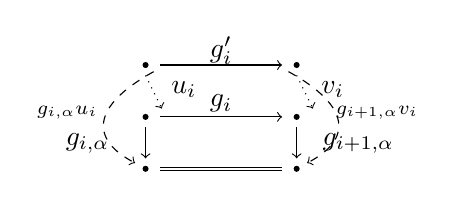
\begin{tikzpicture}[x=2.1em,y=1.5em]
  \fill (0,2.5) circle (1.1pt);
  \fill (2.6,2.5) circle (1.1pt);
  \fill (0,1.25) circle (1.1pt);
  \fill (2.6,1.25) circle (1.1pt);
  \fill (0,0) circle (1.1pt);
  \fill (2.6,0) circle (1.1pt);
  \draw[->] (0.25,2.5) -- (2.35,2.5);
  \node at (1.3,2.84) {$g'_i$};
  \draw[->] (0.25,1.25) -- (2.35,1.25);
  \node at (1.3,1.57) {$g_i$};
  \draw[double] (0.25,0) -- (2.35,0);
  \draw[->,dotted] (0,2.25) -- (0.28,1.45);
  \node at (0.66,1.9) {$u_i$};
  \draw[->,dotted] (2.6,2.25) -- (2.88,1.45);
  \node at (3.22,1.9) {$v_i$};
  \draw[->] (0,1.0) -- (0,0.25);
  \node at (-1.0,0.62) {$g_{i,\alpha}$};
  \draw[->] (2.6,1.0) -- (2.6,0.25);
  \node at (3.66,0.62) {$g_{i+1,\alpha}$};
  \draw[->,dashed] (0.14,2.34) .. controls (-0.95,1.5) and (-0.95,0.7) .. (-0.18,0.14);
  \node at (-1.35,1.35) {$\scriptstyle g_{i,\alpha}u_i$};
  \draw[->,dashed] (2.46,2.34) .. controls (3.55,1.5) and (3.55,0.7) .. (2.78,0.14);
  \node at (3.98,1.35) {$\scriptstyle g_{i+1,\alpha}v_i$};
  \node at (2.3,1.48) {$\lrcorner$};
\end{tikzpicture}
\end{center}
我们把这一立方诠释为：前面那个方块是后面那个方块的推出，而后者分解为相似
方块的余积——$g'_i=\coprod_{J}g'_{i,j}$ 的每个分量各对应一个。由此我们看出：
$g=g_{0,\alpha}$ 是某个\trDiagram{} $\alpha\to\mathcal{M}^{2}$ 之余极限的
定义域分量，这个\trDiagram{}的每一步都是\trCategoryOfArrows{}中映射之余积的
推出。现在 $f\widehat{\otimes}-\colon\mathcal{M}^{2}\to\mathcal{N}^{2}$ 保持%
\trCategoryOfArrows{}中的\trColimit，而定义域函子
$\mathrm{dom}\colon\mathcal{N}^{2}\to\mathcal{N}$ 也保持余极限。于是，
$f\widehat{\otimes}g$ 是诸映射 $f\widehat{\otimes}g'_{i,j}$ 之余积的推出的一个
$\alpha$-序列的余极限。

确立这些断言的更多细节见 \cite[\S4--\S5]{bib107}。
\end{proof}

\begin{definition}\label{def:left-leibniz-bifunctor}
设 $\mathcal{V}$、$\mathcal{M}$ 与 $\mathcal{N}$ 是余完备\trCategory，各自配备
弱分解系统 $(\mathrm{L},\mathrm{R})$、$(\mathrm{L}',\mathrm{R}')$ 与
$(\mathrm{L}'',\mathrm{R}'')$。一个\textbf{左 Leibniz \trBifunctor}（left
Leibniz bifunctor）是一个\trBifunctor{}
$\otimes\colon\mathcal{V}\times\mathcal{M}\to\mathcal{N}$，它
\begin{enumerate}[label=(\roman*)]
\item 在每个变量中分别余连续，并且
\item 具有\textbf{Leibniz 性质}（Leibniz property）：$\mathrm{L}$ 中一个映射
  与 $\mathrm{L}'$ 中一个映射的 $\otimes$-推出积落在 $\mathrm{L}''$ 中。
\end{enumerate}
\end{definition}

对偶地，配备弱分解系统的诸完备\trCategory{}之间的一个\trBifunctor{}是
\textbf{右 Leibniz \trBifunctor}（right Leibniz bifunctor），若它在每个变量中
分别连续，且右类中诸映射的拉回余张量落入右类。我们最常在\trBifunctor
\[ \{,\}\colon\mathcal{V}^{\mathrm{op}}\times\mathcal{N}\to\mathcal{M} \]
的情形下应用这一定义——它在其中一个变量上反变，此时相关的假设为：$\mathcal{V}$
余完备，且第一个变量中的余极限被携带为 $\mathcal{M}$ 中的\trLimit；此外，
$\mathrm{L}$ 中一个映射与 $\mathrm{R}''$ 中一个映射的\trLeibnizCotensor{}定义
$\mathrm{R}'$ 中的一个映射。左、右 Leibniz \trBifunctor{}之间的对偶性的本质
说起来颇为微妙，我们把它留作读者的一道谜题（或见 \cite{bib26}）。

\begin{lemma}\label{lem:leibniz-two-variable-adjunction}
若诸\trBifunctor
\[ \mathcal{V}\times\mathcal{M}\xrightarrow{\;\otimes\;}\mathcal{N},\qquad
   \mathcal{V}^{\mathrm{op}}\times\mathcal{N}\xrightarrow{\;\{,\}\;}
   \mathcal{M},\qquad\text{以及}\qquad
   \mathcal{M}^{\mathrm{op}}\times\mathcal{N}\xrightarrow{\;\mathrm{hom}\;}
   \mathcal{V} \]
定义一个双变量\trAdjunction，而 $(\mathrm{L},\mathrm{R})$、
$(\mathrm{L}',\mathrm{R}')$ 与 $(\mathrm{L}'',\mathrm{R}'')$ 分别是
$\mathcal{V}$、$\mathcal{M}$ 与 $\mathcal{N}$ 上的三个弱分解系统，则下列诸
条件等价：
\begin{enumerate}[label=(\roman*)]
\item $\otimes\colon\mathcal{V}\times\mathcal{M}\to\mathcal{N}$ 定义一个左
  Leibniz \trBifunctor；
\item $\{,\}\colon\mathcal{V}^{\mathrm{op}}\times\mathcal{N}\to\mathcal{M}$
  定义一个右 Leibniz \trBifunctor；
\item $\mathrm{hom}\colon\mathcal{M}^{\mathrm{op}}\times\mathcal{N}\to\mathcal{V}$
  定义一个右 Leibniz \trBifunctor。
\end{enumerate}
当这些条件成立时，我们说 $(\otimes,\{,\},\mathrm{hom})$ 定义一个
\textbf{Leibniz 双变量\trAdjunction}（Leibniz two-variable adjunction）。
\end{lemma}
\begin{proof}
伴随的存在保证每个\trBifunctor{}都满足所需的（余）连续性假设。注意，例如
$\mathrm{L}\widehat{\otimes}\mathrm{L}'\subset\mathrm{L}''$ 当且仅当
$\mathrm{L}\widehat{\otimes}\mathrm{L}'\llsq\mathrm{R}''$。于是三个陈述的%
等价由下述三个提升性质的等价得到：
\[ \mathrm{L}\widehat{\otimes}\mathrm{L}'\llsq\mathrm{R}''
   \quad\leftrightsquigarrow\quad
   \mathrm{L}'\llsq\widehat{\{\mathrm{L},\mathrm{R}''\}}
   \quad\leftrightsquigarrow\quad
   \mathrm{L}\llsq\widehat{\mathrm{hom}}(\mathrm{L}',\mathrm{R}''), \]
其证明留作\cref{ex:leibniz-lifting-equivalences}。
\end{proof}

\begin{remark}\label{rem:leibniz-generators}
由\cref{prop:leibniz-construction-preserves}(vii)，为证一个余连续\trBifunctor{}
$\otimes$ 满足 Leibniz 性质，只需证诸生成态射的 $\otimes$-\trLeibnizProduct{}落在陪域
弱分解系统的左类之中。
\end{remark}

\begin{lemma}\label{lem:set-tensor-leibniz}
对任何带积与余积、并配备弱分解系统 $(\mathrm{L},\mathrm{R})$ 的\trCategory{}
$\mathcal{M}$，集合张量、集合余张量与 hom
\[ \ast\colon\mathcal{S}et\times\mathcal{M}\to\mathcal{M},\qquad
   \{,\}\colon\mathcal{S}et^{\mathrm{op}}\times\mathcal{M}\to\mathcal{M},
   \qquad\text{以及}\qquad
   \mathrm{hom}\colon\mathcal{M}^{\mathrm{op}}\times\mathcal{M}\to\mathcal{S}et \]
相对于 $\mathcal{S}et$ 上的（\trMonomorphism，\trEpimorphism）弱分解系统
分别定义一个 Leibniz 双变量\trAdjunction。
\end{lemma}
\begin{proof}
由\cref{lem:leibniz-two-variable-adjunction}，只需证这些\trBifunctor{}中的
任何一个都是 Leibniz 的。当 $A\hookrightarrow B$ 是 $\mathcal{S}et$ 中的%
\trMonomorphism{}时，与 $f\colon X\to Y$ 的\trLeibnizTensor{}分解为显然落在
$\mathrm{L}$ 中的映射之余积：
\begin{rveq}\label{eq:set-tensor-leibniz-square}
\mbox{\begin{tikzpicture}[x=2.15em,y=1.55em]
  \node (AX) at (0,1.7) {$A\ast X$};
  \node (BX) at (4.6,1.7) {$B\ast X\cong A\ast X\sqcup B\setminus A\ast X$};
  \node (AY) at (0,0.2) {$A\ast Y$};
  \node (MY) at (4.6,0.2) {$A\ast Y\sqcup B\setminus A\ast X$};
  \node (BY) at (9.8,-0.35) {$B\ast Y\cong A\ast Y\sqcup B\setminus A\ast Y$};
  \draw[right hook->] (0.75,1.7) -- (2.0,1.7);
  \draw[->] (0,1.35) -- (0,0.55);
  \node at (-0.8,0.95) {$\scriptstyle A\ast f$};
  \draw[->] (4.6,1.35) -- (4.6,0.55);
  \node at (5.85,0.95) {$\scriptstyle A\ast f\sqcup\mathrm{id}$};
  \draw[->] (0.7,0.2) -- (2.6,0.2);
  \node at (3.5,0.46) {$\lrcorner$};
  \draw[->,dashed] (6.7,0.08) -- (7.85,-0.28);
  \node at (6.75,-0.56) {$\scriptstyle\mathrm{id}\sqcup B\setminus A\ast f$};
  \draw[->] (5.9,1.52) .. controls (8.1,1.25) and (9.6,0.65) .. (9.9,-0.02);
  \node at (8.35,0.98) {$\scriptstyle B\ast f$};
  \draw[->] (0.62,0.02) .. controls (3.0,-0.9) and (6.9,-1.0) .. (7.9,-0.5);
\end{tikzpicture}}
\end{rveq}
一个更利落的证明也是可能的。由于每个\trMonomorphism{}都可表示为由单个%
\trCell{} $\varnothing\hookrightarrow 1$ 构筑起来的胞腔复形，由%
\cref{prop:leibniz-construction-preserves}(vii)，只需考虑与生成\trMonomorphism{}
$\varnothing\hookrightarrow 1$ 的\trLeibnizTensor。但注意\trFunctor
\[ \mathcal{M}^{2}\xrightarrow{\;(\varnothing\hookrightarrow 1)\widehat{\ast}-\;}
   \mathcal{M}^{2} \]
自然\trIsomorphism{}于恒等\trFunctor，而后者当然保持左类 $\mathrm{L}$。
\end{proof}

\begin{remark}\label{rem:hom-right-leibniz}
由\cref{lem:set-tensor-leibniz}，
$\mathrm{hom}\colon\mathcal{M}^{\mathrm{op}}\times\mathcal{M}\to\mathcal{S}et$
是右 Leibniz 的，意即对任何 $\ell\in\mathrm{L}$ 与 $r\in\mathrm{R}$，态射
\[ \mathcal{M}(\mathrm{cod}\,\ell,\mathrm{dom}\,r)
   \xrightarrow{\;r\circ-\circ\ell\;}
   \mathcal{M}(\mathrm{dom}\,\ell,\mathrm{dom}\,r)
   \underset{\mathcal{M}(\mathrm{dom}\,\ell,\mathrm{cod}\,r)}{\times}
   \mathcal{M}(\mathrm{cod}\,\ell,\mathrm{cod}\,r) \]
是一个\trEpimorphism。这个映射的目标是 $\mathcal{M}$ 中从 $\ell$ 到 $r$ 的
交换方块之集，而其在任一元素上的\trFiber{}则是如此呈现的\trLifting{}问题之
解集。这一映射是\trEpimorphism{}这一事实重新表述了提升性质
$\mathrm{L}\llsq\mathrm{R}$。
\end{remark}

\subsection*{练习}

\begin{exercise}\label{ex:finish-closure-proof}
完成\cref{lem:right-lifting-closure}的证明。
\end{exercise}

\begin{exercise}\label{ex:retract-argument}
\begin{enumerate}[label=(\roman*)]
\item 证明「\trRetract{}论证」（retract argument）：设 $f=r\circ\ell$ 且 $f$
  对其右因子 $r$ 具有左\trLifting{}性质，则 $f$ 是其左因子 $\ell$ 的%
  \trRetract。
\item 据此得出：在\cref{def:weak-factorization-system}(i) 与 (ii) 存在时，
  (iii) 可代之以类 $\mathrm{L}$ 与 $\mathrm{R}$ 对收缩封闭这一假设。
\end{enumerate}
\end{exercise}

\begin{exercise}\label{ex:prove-adjunction-transposes}
证明\cref{lem:adjunction-transposes-lifting}。
\end{exercise}

\begin{exercise}\label{ex:inverse-category-diagram-wfs}
\begin{enumerate}[label=(\roman*)]
\item 设 $\mathcal{M}$ 是带\trProduct、\trPullback{}与塔之\trLimit{}的%
  \trCategory，配备弱分解系统 $(\mathrm{L},\mathrm{R})$。证明：对任何逆范畴
  $\mathcal{J}$，图表\trCategory{} $\mathcal{M}^{\mathcal{J}}$ 具有弱分解系统，
  其左类由诸分量皆为 $\mathrm{L}$ 中映射的映射组成，其右类由这样一些映射
  $\alpha\colon X\to Y$ 组成：对每个 $i\in\mathcal{J}$，相对匹配映射
  $\widehat{m}_i\colon X_i\to\partial_iX\underset{\partial_iY}{\times}Y_i$ 落在 $\mathrm{R}$ 中。
\item 在「$\mathcal{M}$ 的类 $\mathrm{F}$ 与 $\mathrm{F}\cap\mathrm{W}$ 是弱
  分解系统的右类」这一附加假设下，给出 $\lim\colon\mathcal{M}^{\mathcal{J}}\to\mathcal{M}$ 保持\trFibration{}与\trTrivialFibration{}的一个新证明。
\end{enumerate}
\end{exercise}

\begin{exercise}\label{ex:leibniz-lifting-equivalences}
给定双变量\trAdjunction{} \eqref{eq:two-variable-adjunction-functors} 与
$\mathcal{V}$、$\mathcal{M}$、$\mathcal{N}$ 中的映射类 $\mathrm{A}$、
$\mathrm{B}$、$\mathrm{C}$，证明下列提升性质等价：
\[ \mathrm{A}\widehat{\otimes}\mathrm{B}\llsq\mathrm{C}
   \quad\Leftrightarrow\quad
   \mathrm{B}\llsq\widehat{\{\mathrm{A},\mathrm{C}\}}
   \quad\Leftrightarrow\quad
   \mathrm{A}\llsq\widehat{\mathrm{hom}}(\mathrm{B},\mathrm{C}). \]
\end{exercise}

   %

\providecommand{\rvC}{\mathbf{C}}  %
\providecommand{\rvW}{\mathbf{W}}  %
\providecommand{\rvF}{\mathbf{F}}  %
\providecommand{\rvWarrow}{\rightsquigarrow}%
\providecommand{\rvFarrow}{\twoheadrightarrow}%
\providecommand{\rvTFarrow}{\rightsquigarrow\joinrel\twoheadrightarrow}%
\providecommand{\rvCarrow}{\rightarrowtail}%
\providecommand{\rvTCarrow}{\rightarrowtail\joinrel\rightsquigarrow}%

\section{模型范畴与 Quillen 函子}\label{sec:model-categories-and-quillen-functors}

下面对 Quillen 的「闭模型范畴」（closed model category）定义%
\cite[I.5.1.1]{bib93} 的重新表述由 Joyal 与 Tierney 给出 \cite[7.7]{bib64}，他们%
证明了：一个配有满足\trTwoOfThreeProperty{}的\trWeakEquivalence{}的\trCategory{}
$(\mathcal{M},\rvW)$ 容有一个\trModelStructure，恰在存在定义如下一对%
\trWeakFactorizationSystem{}的类 $\rvC$ 与 $\rvF$ 时：

\begin{definition}[模型范畴]\label{def:model-structure}
一个\trComplete{}且\trCocomplete{}的\trCategory{} $\mathcal{M}$ 上的一个%
\textbf{\trModelStructure}由映射的三个类构成——\textbf{\trWeakEquivalence}
$\rvW$（记作「$\rvWarrow$」），它必须满足\trTwoOfThreeProperty；\textbf{余纤维
化}（cofibration）$\rvC$（记作「$\rvCarrow$」）；以及\textbf{\trFibration}
$\rvF$（记作「$\rvFarrow$」）——使得 $(\rvC,\rvF\cap\rvW)$ 与
$(\rvC\cap\rvW,\rvF)$ 各自在 $\mathcal{M}$ 上定义一个\trWeakFactorizationSystem。%
\footnote{在\trModelCategory{}的诸标准定义中有一条公理——\trWeakEquivalence{}对%
\trRetract{}的封闭性——并未显然地被打包进这些假设之中，但它是此处所给诸公理的
一个推论 \cite[7.8]{bib64}。}

一个\textbf{\trModelCategory}是一个配有\trModelStructure{}的\trComplete{}且%
\trCocomplete{}的\trCategory。\trModelCategory{}中表现更佳的对象或「\trFibrant」、
或「\trCofibrant」、或两者兼备：
\end{definition}

\begin{definition}\label{def:fibrant-cofibrant}
在\trModelCategory{} $\mathcal{M}$ 中，一个对象 $X$ 是\textbf{\trFibrant}的，恰在%
从它到\trTerminal{}对象的唯一映射 $X\to 1$ 是一支\trFibration{}时；是%
\textbf{\trCofibrant}的，恰在从\trInitial{}对象出发的唯一映射%
$\varnothing\to X$ 是一支余纤维化时。经由分解这些唯一映射，任何对象 $X$ 都拥有按
如下方式构造的一个\textbf{余纤维性替换}（cofibrant replacement）$QX$ 与一个%
\textbf{纤维性替换}（fibrant replacement）$RX$：
\begin{center}
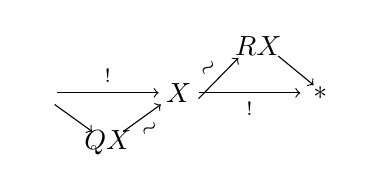
\begin{tikzpicture}[x=1.6em,y=1.4em]
  \node (RX) at (5.0,2.5) {$RX$};
  \node (empty) at (0,1.3) {$\varnothing$};
  \node (X) at (3.2,1.3) {$X$};
  \node (star) at (6.4,1.3) {$\ast$};
  \node (QX) at (1.6,0) {$QX$};
  \draw[->] (0.45,1.3) -- (2.75,1.3);
  \node at (1.6,1.74) {$\scriptstyle !$};
  \draw[->] (3.65,1.15) -- (4.55,2.2) node[midway,above,sloped]{$\scriptstyle\sim$};
  \draw[->] (5.45,2.25) -- (6.25,1.5);
  \draw[->] (3.65,1.3) -- (5.95,1.3);
  \node at (4.8,0.9) {$\scriptstyle !$};
  \draw[->] (0.4,1.0) -- (1.25,0.3);
  \draw[->] (1.95,0.3) -- (2.8,1.0) node[midway,below,sloped]{$\scriptstyle\sim$};
\end{tikzpicture}
\end{center}
\end{definition}

请注意，\cref{def:weak-factorization-system}与\cref{def:model-structure}是自对
偶的：若 $(\mathrm{L},\mathrm{R})$ 定义 $\mathcal{M}$ 上的一个\trWeakFactorizationSystem，则
$(\mathrm{R},\mathrm{L})$ 定义 $\mathcal{M}^{\mathrm{op}}$ 上的一个\trWeakFactorizationSystem。
于是，关于\trFibration{}之右类 $\rvF$ 与\textbf{\trTrivialFibration}%
「$\rvTFarrow$」之右类 $\rvF\cap\rvW$ 的一切一般性定理，都蕴涵涉及余纤维化之左类
$\rvC$ 与\textbf{平凡余纤维化}（trivial cofibration）「$\rvTCarrow$」之左类
$\rvC\cap\rvW$ 的诸对偶结果。特别地，由\cref{exa:model-category-fibrant-objects}，
C.1 节中所证明的关于一个\trCategoryOfFibrantObjects{}的全部结果，对于\trModelCategory{}中由此
得名的诸\trFibrant{}对象之间的\trFibration、\trTrivialFibration{}与%
\trWeakEquivalence{}都成立，而这些结果的诸对偶对于\trCofibrant{}对象之间的余纤
维化、平凡余纤维化与\trWeakEquivalence{}亦成立。

还请注意：既然\trWeakFactorizationSystem{}的任何一个类都确定另一个类，平凡余纤维化便可以在既不参
照余纤维化也不参照\trWeakEquivalence{}的情况下定义出来——即那些对诸%
\trFibration{}具有左\trLifting{}性质的映射；对偶地，\trTrivialFibration{}恰是那
些对诸余纤维化具有右\trLifting{}性质的映射。

\begin{definition}\label{def:quillen-functor}
介于诸\trModelCategory{}之间的一个\trFunctor{}是
\begin{itemize}
\item \textbf{左 Quillen}的，若它保持余纤维化、平凡余纤维化与\trCofibrant{}对
  象；并且
\item \textbf{右 Quillen}的，若它保持\trFibration、\trTrivialFibration{}与%
\trFibrant{}对象。
\end{itemize}
\end{definition}

左 Quillen \trFunctor{}容有左导出函子，而右 Quillen \trFunctor{}容有右导出函子。
为免于定义这些术语，我们把这方面的完整论述留给其他作者 \cite[§2.1--2]{bib103}，
但 Quillen \trFunctor{}之「可导出性」的一个重要成分已由下述结果所捕捉：

\begin{lemma}\label{lem:quillen-preserves-we}
介于诸\trModelCategory{}之间的任何左 Quillen \trFunctor{}都保持\trCofibrant{}对
象之间的\trWeakEquivalence，而任何右 Quillen \trFunctor{}都保持\trFibrant{}对象
之间的\trWeakEquivalence。
\end{lemma}
\begin{proof}
对右 Quillen \trFunctor{}而言，这直接由\cref{lem:ken-brown}与%
\cref{exa:model-category-fibrant-objects}得出。左 Quillen \trFunctor{}的结果是对
偶的。
\end{proof}

大多数左 Quillen \trFunctor{}都是「余连续的」，保持一切\trColimit；而大多数右
Quillen \trFunctor{}都是「连续的」，保持一切\trLimit；当情形如此时，便无须另行
假设\trCofibrant{}对象或\trFibrant{}对象被保持。事实上，Quillen \trFunctor{}通常
以\trAdjunction{}对的形态出现：

\begin{definition}\label{def:quillen-adjunction}
试考虑介于一对\trModelCategory{}之间的一个\trAdjunction
\begin{center}
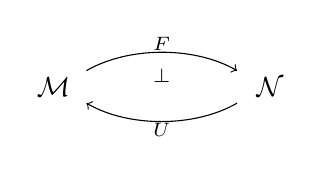
\begin{tikzpicture}[x=1.7em,y=1.4em]
  \node (M) at (0,0) {$\mathcal{M}$};
  \node (N) at (4.6,0) {$\mathcal{N}$};
  \draw[->] (0.7,0.42) .. controls (1.6,1.05) and (3.0,1.05) .. (3.9,0.42);
  \node at (2.3,1.12) {$\scriptstyle F$};
  \node at (2.3,0.28) {$\scriptstyle\bot$};
  \draw[->] (3.9,-0.42) .. controls (3.0,-1.05) and (1.6,-1.05) .. (0.7,-0.42);
  \node at (2.3,-1.12) {$\scriptstyle U$};
\end{tikzpicture}
\end{center}
由\cref{lem:adjunction-transposes-lifting}，下列诸条件等价，它们定义一个%
\textbf{Quillen \trAdjunction}（Quillen adjunction）：
\begin{enumerate}[label=(\roman*)]
\item \trLeftAdjoint{} $F$ 是左 Quillen 的。
\item \trRightAdjoint{} $U$ 是右 Quillen 的。
\item \trLeftAdjoint{}保持余纤维化，而\trRightAdjoint{}保持\trFibration。
\item \trLeftAdjoint{}保持平凡余纤维化，而\trRightAdjoint{}保持%
\trTrivialFibration。
\end{enumerate}
\end{definition}

\begin{lemma}\label{lem:quillen-equivalence}
对于一个 Quillen \trAdjunction
\begin{center}
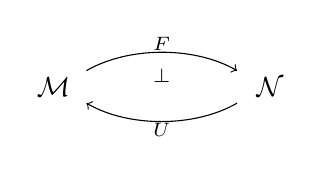
\begin{tikzpicture}[x=1.7em,y=1.4em]
  \node (M) at (0,0) {$\mathcal{M}$};
  \node (N) at (4.6,0) {$\mathcal{N}$};
  \draw[->] (0.7,0.42) .. controls (1.6,1.05) and (3.0,1.05) .. (3.9,0.42);
  \node at (2.3,1.12) {$\scriptstyle F$};
  \node at (2.3,0.28) {$\scriptstyle\bot$};
  \draw[->] (3.9,-0.42) .. controls (3.0,-1.05) and (1.6,-1.05) .. (0.7,-0.42);
  \node at (2.3,-1.12) {$\scriptstyle U$};
\end{tikzpicture}
\end{center}
下列诸条件等价，并且刻画了那些定义\textbf{Quillen \trEquivalence}（Quillen
equivalence）的 Quillen \trAdjunction：
\begin{enumerate}[label=(\roman*)]
\item 对每个\trCofibrant{}对象 $M\in\mathcal{M}$ 与每个\trFibrant{}对象
  $N\in\mathcal{N}$，映射 $f^{\sharp}\colon FM\to N$ 是 $\mathcal{N}$ 中的%
\trWeakEquivalence，当且仅当其转置 $f^{\flat}\colon M\to UN$ 是 $\mathcal{M}$ 中
的\trWeakEquivalence。
\item 对每个\trCofibrant{}对象 $M\in\mathcal{M}$，导出单位（derived unit）
  \[ M\xrightarrow{\ \eta\ }UFM\longrightarrow URFM \]
  ——由\trUnit{}与纤维性替换复合而定义——是\trWeakEquivalence；并且对每个%
\trFibrant{}对象 $N\in\mathcal{N}$，导出余单位（derived counit）
  \[ FQUN\longrightarrow FUN\xrightarrow{\ \varepsilon\ }N \]
  ——由\trCounit{}与余纤维性替换复合而定义——是\trWeakEquivalence。
\end{enumerate}
\end{lemma}

\begin{proof}
假设 (i) 成立，并试考虑一个\trCofibrant{}对象 $M\in\mathcal{M}$ 与一个%
\trFibrant{}对象 $N\in\mathcal{N}$。导出单位与导出余单位分别是纤维性替换映射与余
纤维性替换映射的转置
\[ FM\;\rvWarrow\;RFM \qquad\qquad QUN\;\rvWarrow\;UN \]
由\cref{def:fibrant-cofibrant}，这些映射是\trWeakEquivalence；既然 $M$ 与 $QUN$
是\trCofibrant{}的而 $RFM$ 与 $N$ 是\trFibrant{}的，(i) 便告诉我们：导出单位与导
出余单位也必是\trWeakEquivalence。

现在假设导出单位是\trWeakEquivalence，并试考虑\trWeakEquivalence{}
$f^{\sharp}\colon FM\rvWarrow N$，其中 $M$ 是\trCofibrant{}的而 $N$ 是%
\trFibrant{}的。施用\trRightAdjoint{}与纤维性替换，我们得到一个交换\trDiagram
\begin{center}
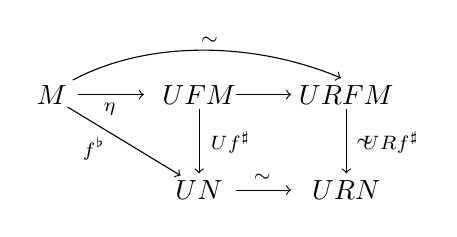
\begin{tikzpicture}[x=1.9em,y=1.5em]
  \node (M) at (0,2.3) {$M$};
  \node (UFM) at (2.8,2.3) {$UFM$};
  \node (URFM) at (5.6,2.3) {$URFM$};
  \node (UN) at (2.8,0) {$UN$};
  \node (URN) at (5.6,0) {$URN$};
  \draw[->] (0.5,2.3) -- (1.75,2.3);
  \node at (1.1,1.95) {$\scriptstyle\eta$};
  \draw[->] (3.5,2.3) -- (4.55,2.3);
  \draw[->] (0.4,2.65) .. controls (1.8,3.6) and (3.8,3.6) .. (5.5,2.7);
  \node at (3.0,3.6) {$\scriptstyle\sim$};
  \draw[->] (0.3,2.0) -- (2.45,0.35);
  \node at (0.8,1.0) {$\scriptstyle f^{\flat}$};
  \draw[->] (2.8,1.95) -- (2.8,0.4);
  \node at (3.4,1.15) {$\scriptstyle Uf^{\sharp}$};
  \draw[->] (5.6,1.95) -- (5.6,0.4);
  \node at (5.95,1.15) {$\scriptstyle\sim$};
  \node at (6.45,1.15) {$\scriptstyle URf^{\sharp}$};
  \draw[->] (3.5,0) -- (4.55,0);
  \node at (4.0,0.3) {$\scriptstyle\sim$};
\end{tikzpicture}
\end{center}
由\cref{lem:quillen-preserves-we}，右边与底部的映射是\trWeakEquivalence，而由假
设，作为顶部复合出现的导出单位亦然。由\trTwoOfThreeProperty，转置
$f^{\flat}\colon M\rvWarrow UN$ 也是\trWeakEquivalence。对偶地，若导出余单位是%
\trWeakEquivalence，则\trWeakEquivalence{} $f^{\flat}\colon M\rvWarrow UN$ 经转
置给出\trWeakEquivalence{} $f^{\sharp}\colon FM\rvWarrow N$。
\end{proof}

现在我们在\trDiagram{}\trCategory{}上引入一对\trModelStructure，其设计用意在于
保证对角\trFunctor{} $\Delta\colon\mathcal{M}\to\mathcal{M}^{\mathcal{J}}$ 分别
是右 Quillen 的或左 Quillen 的，从而\trColimit{}\trFunctor{}与\trLimit{}\trFunctor{}%
分别是左 Quillen 的或右 Quillen 的。相应的左、右导出函子随后便定义%
\textbf{\trHomotopyColimit}（homotopy colimit）与\textbf{\trHomotopyLimit}
（homotopy limit）\trFunctor。

\begin{definition}\label{def:projective-injective-model-structures}
设 $\mathcal{M}$ 是一个\trModelCategory，并设 $\mathcal{J}$ 是一个小范畴（small
category）。
\begin{enumerate}[label=(\roman*)]
\item $\mathcal{M}^{\mathcal{J}}$ 上的\textbf{射影模型结构}（projective model
  structure）的\trWeakEquivalence{}与\trFibration{}在 $\mathcal{M}$ 中逐点定义。
\item $\mathcal{M}^{\mathcal{J}}$ 上的\textbf{\trInjectiveModelStructure}（injective model
  structure）的\trWeakEquivalence{}与余纤维化在 $\mathcal{M}$ 中逐点定义。
\end{enumerate}
\end{definition}

当\trModelCategory{} $\mathcal{M}$ 是\emph{组合的}（combinatorial）或更一般的%
\emph{\trAccessible}（accessible）时，射影与\trInjectiveModelStructure{}总是存在 \cite{bib54}。
当然，即便没有这些假设，射影与\trInjectiveModelStructure{}也可能碰巧存在于
$\mathcal{M}^{\mathcal{J}}$ 之上——或许对特定的\trDiagram{}形状 $\mathcal{J}$
如此。

一个 Quillen 双变量伴随是这样的双变量\trAdjunction：其\trLeftAdjoint{}是一个左
Quillen \trBifunctor，而其诸\trRightAdjoint{}都是右 Quillen \trBifunctor。由%
\cref{ex:leibniz-lifting-equivalences}，这些条件中的任何一个都蕴涵其余两个：

\begin{definition}\label{def:quillen-two-variable-adjunction}
一个双变量\trAdjunction
\[ \mathcal{V}\times\mathcal{M}\xrightarrow{\ \otimes\ }\mathcal{N},\qquad
   \mathcal{V}^{\mathrm{op}}\times\mathcal{N}\xrightarrow{\ \{,\}\ }\mathcal{M},
   \qquad
   \mathcal{M}^{\mathrm{op}}\times\mathcal{N}\xrightarrow{\ \mathrm{hom}\ }\mathcal{V} \]
介于\trModelCategory{} $\mathcal{V}$、$\mathcal{M}$ 与 $\mathcal{N}$ 之间。若下
列等价条件中的任何一个——从而全部——得到满足，则它定义一个\textbf{Quillen 双
变量\trAdjunction}（Quillen two-variable adjunction）：
\begin{enumerate}[label=(\roman*)]
\item \trFunctor{} $\widehat{\otimes}\colon\mathcal{V}^{\mathbf{2}}\times\mathcal{M}^{\mathbf{2}}\to\mathcal{N}^{\mathbf{2}}$ 把 $\mathcal{V}$ 中一支余
  纤维化与 $\mathcal{M}$ 中一支余纤维化载为 $\mathcal{N}$ 中一支余纤维化，进而当
  两支定义域余纤维化中有任何一支是\trWeakEquivalence{}时，这支余纤维化也是%
\trWeakEquivalence。
\item \trFunctor{} $\widehat{\{,\}}\colon(\mathcal{V}^{\mathbf{2}})^{\mathrm{op}}\times\mathcal{N}^{\mathbf{2}}\to\mathcal{M}^{\mathbf{2}}$ 把 $\mathcal{V}$ 中一支余
  纤维化与 $\mathcal{N}$ 中一支\trFibration{}载为 $\mathcal{M}$ 中一支%
\trFibration，进而当两支定义域映射中有任何一支是\trWeakEquivalence{}时，这支%
\trFibration{}也是\trWeakEquivalence。%
  \footnote{原书于此印作「to a fibration in $\mathcal{N}$」；按该函子之值域为
  $\mathcal{M}^{\mathbf{2}}$，疑为 $\mathcal{M}$ 之误，此处径改。——译者注}
\item \trFunctor{} $\widehat{\mathrm{hom}}\colon(\mathcal{M}^{\mathbf{2}})^{\mathrm{op}}\times\mathcal{N}^{\mathbf{2}}\to\mathcal{V}^{\mathbf{2}}$ 把 $\mathcal{M}$ 中
  一支余纤维化与 $\mathcal{N}$ 中一支\trFibration{}载为 $\mathcal{V}$ 中一支%
\trFibration，进而当两支定义域映射中有任何一支是\trWeakEquivalence{}时，这支%
\trFibration{}也是\trWeakEquivalence。
\end{enumerate}
\end{definition}

\begin{remark}\label{rem:left-quillen-bifunctor}
由\cref{def:quillen-two-variable-adjunction}，一个双变量\trAdjunction{}是 Quillen
的，当且仅当其\trLeftAdjoint{} $\otimes\colon\mathcal{V}\times\mathcal{M}\to\mathcal{N}$
是一个\textbf{左 Quillen \trBifunctor}（left Quillen bifunctor）：
一个相对于诸构成性\trWeakFactorizationSystem{}的八种可能选取中的七种为左 Leibniz 的%
\trBifunctor——唯一的例外是对 $\mathcal{V}$ 与 $\mathcal{M}$ 都选取
$(\rvC,\rvF\cap\rvW)$、而对 $\mathcal{N}$ 选取 $(\rvC\cap\rvW,\rvF)$ 的那一种
选取。
\end{remark}

Quillen 对其单纯集范畴上的\trModelStructure{}所享有的附加性质所作的公理化，已被
Hovey \cite[§4.2]{bib57} 加以推广，以定义幺半模型范畴与富集模型范畴的概念。我们
把前者特化到 A.1 节的那些\trCartesianClosed{}范畴——因为此处需要的只有这些情形。
若 $\mathcal{V}$ 具有一个\trModelStructure、同时也是一个\trCartesianClosed{}范
畴，则自然要问这些结构是否相容，其意义如下：

\begin{definition}\label{def:cartesian-closed-model-category}
一个\textbf{笛卡尔封闭的模型范畴}（cartesian closed model category）是一个%
\trCartesianClosed{}范畴 $(\mathcal{V},\times,1)$ 配上一个\trModelStructure，使得
\begin{enumerate}[label=(\roman*)]
\item \trCartesianProduct{}与\trInternalHom{}定义一个 Quillen 双变量\trAdjunction；并且
\item 由\trTerminal{}对象的余纤维性替换所定义的映射
  $Q1\times v\to 1\times v\cong v$，在 $v$ 是\trCofibrant{}的时是%
\trWeakEquivalence。
\end{enumerate}
\end{definition}

\begin{definition}\label{def:v-model-category}
若 $\mathcal{V}$ 是一个笛卡尔封闭的模型范畴，则一个\textbf{$\mathcal{V}$-模型范
畴}（$\mathcal{V}$-model category）是一个张量化、余张量化且 $\mathcal{V}$-富集
的\trModelCategory{} $\mathcal{M}$，使得
\begin{enumerate}[label=(\roman*)]
\item $(\otimes,\{,\},\mathrm{hom})$ 是一个 Quillen 双变量\trAdjunction；并且
\item 由\trTerminal{}对象的余纤维性替换所定义的映射
  $Q1\otimes m\to 1\otimes m\cong m$，在 $m$ 是\trCofibrant{}的时是%
\trWeakEquivalence。
\end{enumerate}
\end{definition}

若 $1\in\mathcal{V}$ 是\trCofibrant{}的，则\cref{def:cartesian-closed-model-category}%
与\cref{def:v-model-category}两者中的第二个条件都由第一个条件推出（见%
\cref{ex:quillen-bifunctor-component}）。

\begin{lemma}\label{lem:v-model-hom-fibrant}
若 $\mathcal{M}$ 是一个 $\mathcal{V}$-模型范畴，则对 $\mathcal{M}$ 中任何%
\trCofibrant{}对象 $M$ 与任何\trFibrant{}对象 $N$，$\mathrm{hom}(M,N)$ 是
$\mathcal{V}$ 中的一个\trFibrant{}对象。更一般地，对任何\trCofibrant{}对象 $M$
与任何\trFibration{} $p\colon N\rvFarrow P$，诱导映射
$p_{\ast}\colon\mathrm{hom}(M,N)\to\mathrm{hom}(M,P)$ 是 $\mathcal{V}$ 中的一支%
\trFibration。
\end{lemma}
\begin{proof}
由附录 A 中的\cref{prop:tensors-cotensors-conical}——它对\trTerminal{}对象
$1\in\mathcal{M}$ 与任何 $M\in\mathcal{M}$ 蕴涵 $\mathrm{hom}(M,1)\cong 1$ 在
$\mathcal{V}$ 中是\trTerminal{}的——第二个陈述涵盖第一个陈述。%
\footnote{原书于此印作「any $M\in\mathcal{V}$」；按
$\mathrm{hom}\colon\mathcal{M}^{\mathrm{op}}\times\mathcal{M}\to\mathcal{V}$ 之
型，疑为 $M\in\mathcal{M}$ 之误，此处径改。——译者注}由%
\cref{ex:leibniz-lifting-equivalences}，下方左侧对 $\mathcal{V}$ 中任何平凡余纤维
化 $i$ 的\trLifting{}问题经转置给出下方右侧的\trLifting{}问题
\begin{center}
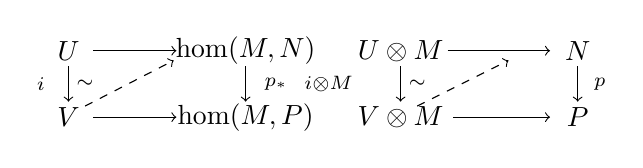
\begin{tikzpicture}[x=2.0em,y=1.6em]
  \node (U1) at (0,1.5) {$U$};
  \node (hMN) at (3.2,1.5) {$\mathrm{hom}(M,N)$};
  \node (V1) at (0,0) {$V$};
  \node (hMP) at (3.2,0) {$\mathrm{hom}(M,P)$};
  \draw[->] (0.45,1.5) -- (1.95,1.5);
  \draw[->] (0.45,0) -- (1.95,0);
  \draw[->] (0,1.15) -- (0,0.35);
  \node at (-0.5,0.75) {$\scriptstyle i$};
  \node at (0.3,0.75) {$\scriptstyle\sim$};
  \draw[->] (3.2,1.15) -- (3.2,0.35);
  \node at (3.75,0.75) {$\scriptstyle p_{\ast}$};
  \draw[->,dashed] (0.3,0.25) -- (1.9,1.28);
  \begin{scope}[shift={(6.0,0)}]
    \node (U2) at (0,1.5) {$U\otimes M$};
    \node (N2) at (3.2,1.5) {$N$};
    \node (V2) at (0,0) {$V\otimes M$};
    \node (P2) at (3.2,0) {$P$};
    \draw[->] (0.85,1.5) -- (2.7,1.5);
    \draw[->] (0.95,0) -- (2.7,0);
    \draw[->] (0,1.15) -- (0,0.35);
    \node at (-1.3,0.75) {$\scriptstyle i\otimes M$};
    \node at (0.3,0.75) {$\scriptstyle\sim$};
    \draw[->] (3.2,1.15) -- (3.2,0.35);
    \node at (3.6,0.75) {$\scriptstyle p$};
    \draw[->,dashed] (0.3,0.25) -- (1.95,1.28);
  \end{scope}
\end{tikzpicture}
\end{center}
由\cref{ex:quillen-bifunctor-component}，既然 $M$ 是\trCofibrant{}的，
$-\otimes M\colon\mathcal{V}\to\mathcal{M}$ 是左 Quillen 的，于是 $i\otimes M$
是 $\mathcal{M}$ 中的一支平凡余纤维化；又因 $p\colon N\rvFarrow P$ 是一支%
\trFibration，该\trLifting{}问题有解。
\end{proof}

下一个结果由 Gambino \cite{bib45} 在一个富集于 Quillen 的单纯集笛卡尔封闭模型结
构之上的\trModelCategory{}的语境中表述，但其证明适用于更大的普遍性。

\begin{theorem}\label{thm:weighted-colimit-limit-quillen}
若 $\mathcal{M}$ 是一个 $\mathcal{V}$-模型范畴且 $\mathcal{J}$ 是一个小范畴，则
加权\trColimit{}\trFunctor
\[ \operatorname{colim}_{--}\colon
   \mathcal{V}^{\mathcal{J}}\times\mathcal{M}^{\mathcal{J}^{\mathrm{op}}}
   \to\mathcal{M} \]
在诸定义域范畴具有（内射，射影）或（射影，内射）模型结构时是左 Quillen 的。类似
地，加权\trLimit{}\trFunctor
\[ \operatorname{lim}_{--}\colon
   (\mathcal{V}^{\mathcal{J}})^{\mathrm{op}}\times\mathcal{M}^{\mathcal{J}}
   \to\mathcal{M} \]
在诸定义域范畴具有（射影，射影）或（内射，内射）模型结构时是右 Quillen 的。
\end{theorem}
\begin{proof}
由\cref{def:quillen-two-variable-adjunction}，我们可以以\trAdjunction{}形式证明
这两个陈述。附录 A 中的\cref{def:weighted-limit-colimit-universal-property}的加
权\trColimit{}\trBifunctor{}容有一个\trRightAdjoint（它被用来表达加权%
\trColimit{}的定义性\trUniversalProperty）
\[ \mathrm{hom}\colon
   (\mathcal{M}^{\mathcal{J}^{\mathrm{op}}})^{\mathrm{op}}\times\mathcal{M}
   \to\mathcal{V}^{\mathcal{J}} \]
它把 $F\in\mathcal{M}^{\mathcal{J}^{\mathrm{op}}}$ 与 $m\in\mathcal{M}$ 送到
$\mathrm{hom}(F-,m)\in\mathcal{V}^{\mathcal{J}}$。

为证 $\mathcal{V}^{\mathcal{J}}$ 具有射影模型结构而
$\mathcal{M}^{\mathcal{J}^{\mathrm{op}}}$ 具有内射\trModelStructure{}时的那个陈述，我们必须
证明：这是一个相对于 $\mathcal{M}^{\mathcal{J}^{\mathrm{op}}}$ 中的逐点（平凡）余
纤维化、$\mathcal{M}$ 中的（平凡）\trFibration{}以及 $\mathcal{V}^{\mathcal{J}}$
中的逐点（平凡）\trFibration{}而言的右 Quillen \trBifunctor。由于右 Quillen %
\trBifunctor{}定义中所涉及的诸\trLimit{}也是逐点构成的，这立即由富集 hom %
\trBifunctor{}的相应性质得出——后者是富集模型范畴定义的一部分。其余诸情形类似。
\end{proof}

\begin{digression}[\trHomotopyColimit{}的构造]\label{dig:homotopy-colimit-construction}
在一个\trModelCategory{}中，术语\emph{\trHomotopyColimit}与\emph{\trHomotopyLimit}
指称\trColimit{}\trFunctor{}与\trLimit{}\trFunctor{}的导出函子。%
\cref{thm:weighted-colimit-limit-quillen}的要旨在于：构造一个%
\trHomotopyColimit{}有两条进路——「增肥\trDiagram」，例如要求其诸对象是%
\trCofibrant{}的且其诸态射是余纤维化——或者「增肥权」，典型做法是取终权的一个余
纤维性替换 \cite[§11.5]{bib103}。第 6 章中的\cref{lem:iso-commas-pullbacks}与%
\cref{lem:iso-towers-flexible}可以被理解为这两种进路之间的一般等价的实例。
\end{digression}

我们从\cref{thm:weighted-colimit-limit-quillen}的众多推论中单独挑出如下一条，其
令人感兴趣之处在于：第 6 章中的\cref{def:flexible-weights}的诸柔性权，恰好就是权
的范畴上相对于单纯集的 Joyal \trModelStructure{}而定义的射影模型结构中的诸%
\trCofibrant{}对象。

\begin{corollary}\label{cor:flexible-weight-fibrant-limit}
若 $\mathcal{M}$ 是一个 $\mathcal{V}$-模型范畴，则对任何对象皆为\trFibrant{}的%
\trDiagram{} $F\in\mathcal{M}^{\mathcal{J}}$ 与任何射影\trCofibrant{}的权
$W\in\mathcal{V}^{\mathcal{J}}$，加权\trLimit{}是一个\trFibrant{}对象。
\end{corollary}
\begin{proof}
由\cref{thm:weighted-colimit-limit-quillen}，加权\trLimit{}\trBifunctor%
$\operatorname{lim}_{--}\colon(\mathcal{V}^{\mathcal{J}})^{\mathrm{op}}\times\mathcal{M}^{\mathcal{J}}\to\mathcal{M}$ 相对于权的范畴上的射影模型结构与%
\trDiagram{}\trCategory{}上的射影模型结构是右 Quillen 的。既然右 Quillen %
\trBifunctor{}保持\trFibrant{}对象，由此得出：由一个射影\trCofibrant{}的权加权的%
\trPointwise{}纤维性图表之\trLimit{}是\trFibrant{}的。
\end{proof}

最后，我们将利用下述定理，它使\trModelCategory{}的富集\trChangeOfBase{}成为可能，
推广了 A.7 节的结果。\cref{thm:change-of-base-quillen-model}的前提是附录 A 中的%
\cref{prop:change-of-base-2-adjunction}的前提到富集模型范畴语境中的显然推广，但其
结论只容许我们沿\trRightAdjoint{}的方向转移富集，因为一个富集模型范畴还必须是张
量化且余张量化的，而这些性质只沿那个方向转移。

下面的结果是把 \cite[3.8]{bib50} 中所证明的一个更一般的定理特化到富集之笛卡尔封闭
基的情形。

\begin{theorem}\label{thm:change-of-base-quillen-model}
试考虑介于诸笛卡尔封闭的模型范畴之间的一个 Quillen \trAdjunction，其中%
\trLeftAdjoint{}保持有限积：
\begin{center}
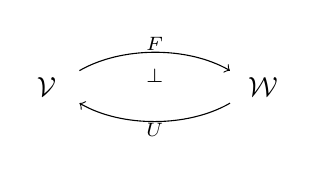
\begin{tikzpicture}[x=1.7em,y=1.4em]
  \node (V) at (0,0) {$\mathcal{V}$};
  \node (W) at (4.6,0) {$\mathcal{W}$};
  \draw[->] (0.7,0.42) .. controls (1.6,1.05) and (3.0,1.05) .. (3.9,0.42);
  \node at (2.3,1.12) {$\scriptstyle F$};
  \node at (2.3,0.28) {$\scriptstyle\bot$};
  \draw[->] (3.9,-0.42) .. controls (3.0,-1.05) and (1.6,-1.05) .. (0.7,-0.42);
  \node at (2.3,-1.12) {$\scriptstyle U$};
\end{tikzpicture}
\end{center}
那么，任何 $\mathcal{W}$-模型范畴都容有成为一个 $\mathcal{V}$-模型范畴的结构，
后者具有同一个底非富集模型范畴，其富集 hom、\trCotensor{}与\trTensor{}由下式
定义：
\[ \mathrm{hom}_{\mathcal{V}}(M,N)\coloneqq U\,\mathrm{hom}_{\mathcal{W}}(M,N),
   \qquad
   V\otimes M\coloneqq FV\otimes M,\qquad\text{以及}\qquad
   M^{V}\coloneqq M^{FV}. \]
\end{theorem}
\begin{proof}
由附录 A 中的\cref{prop:change-of-base-tensored-cotensored}，这些定义使
$\mathcal{M}$\footnote{原书印作「$\mathcal{W}$」，疑为「$\mathcal{M}$」之误——受换基富集者应为该 $\mathcal{W}$-模型范畴本身，此处径改。——译者注}成为一个张量化且余张量化的 $\mathcal{V}$-富集范畴。附录 A 中的%
\cref{lem:change-of-base-underlying-categories}观察到：沿保持有限积的%
\trAdjunction{}之\trRightAdjoint{}所作的换基保持诸底 1-\trCategory。尚须验证的
只是：$\mathcal{V}$-富集 hom、\trTensor{}与\trCotensor{}底下的诸\trFunctor{}定义
一个 Quillen
双变量\trAdjunction，而这容易由\trModelCategory{} $\mathcal{V}$ 与 $\mathcal{W}$ 的笛卡尔
封闭性以及 $F\dashv U$ 是 Quillen 的这一事实得出。
\end{proof}

\subsection*{练习}

\begin{exercise}\label{ex:fibrant-objects-from-model}
验证：一个\trModelCategory{}中\trFibrant{}对象的全子范畴定义一个\trCategoryOfFibrantObjects，
其中取 $\rvW$ 为\trWeakEquivalence{}类、取 $\rvF$ 为\trFibrant{}对象之间的诸%
\trFibration{}的类。
\end{exercise}

\begin{exercise}\label{ex:model-structure-determined}
验证：$\mathcal{M}$ 上的一个\trModelStructure（若它存在的话）由下列诸数据中的任
何一个唯一确定：
\begin{enumerate}[label=(\roman*)]
\item 余纤维化与\trWeakEquivalence；
\item \trFibration{}与\trWeakEquivalence；
\item 余纤维化与\trFibration；或者
\item 平凡余纤维化与\trTrivialFibration。%
  \footnote{据 Joyal 的一个更为精致的观察 \cite[E.1.10]{bib63}，模型结构还由如下
  数据唯一确定：(v) 余纤维化与纤维性对象，或 (vi) 纤维化与余纤维性对象。}
\end{enumerate}
\end{exercise}

\begin{exercise}\label{ex:quillen-bifunctor-component}
\begin{enumerate}[label=(\roman*)]
\item 证明：若 $\otimes\colon\mathcal{V}\times\mathcal{M}\to\mathcal{N}$ 是一个
  左 Quillen \trBifunctor{}且 $V\in\mathcal{V}$ 是\trCofibrant{}的，则
  $V\otimes-\colon\mathcal{M}\to\mathcal{N}$ 是一个左 Quillen \trFunctor。
\item 由此推论：若 $1\in\mathcal{V}$ 是\trCofibrant{}的，则%
  \cref{def:cartesian-closed-model-category}与\cref{def:v-model-category}的第二
  个条件是不必要的。
\end{enumerate}
\end{exercise}

\begin{exercise}\label{ex:set-model-category}
在一个带\trProduct{}与\trCoproduct{}的局部小范畴（locally small category）
$\mathcal{M}$ 中，hom \trBifunctor{}是某个双变量\trAdjunction{}的一部分：
\[ \ast\colon\mathcal{S}et\times\mathcal{M}\to\mathcal{M},\qquad
   \{,\}\colon\mathcal{S}et^{\mathrm{op}}\times\mathcal{M}\to\mathcal{M},\qquad
   \mathrm{hom}\colon\mathcal{M}^{\mathrm{op}}\times\mathcal{M}\to\mathcal{S}et. \]
为 $\mathcal{S}et$ 配备如下\trModelStructure——其\trWeakEquivalence{}是一切映
射、其余纤维化是诸\trMonomorphism、其\trFibration{}是诸\trEpimorphism——并证明：
\begin{enumerate}[label=(\roman*)]
\item $\mathcal{S}et$ 是一个笛卡尔封闭的模型范畴。
\item 任何\trModelCategory{} $\mathcal{M}$ 都是一个 $\mathcal{S}et$-模型范畴。
\end{enumerate}
\end{exercise}

   %

\providecommand{\rvAinc}{\vec{\mathcal{A}}}%
\providecommand{\rvAdec}{\overleftarrow{\mathcal{A}}}%
\providecommand{\wlim}{\operatorname{lim}}%
\providecommand{\wcolim}{\operatorname{colim}}%

\section{作为胞腔复形的 Reedy 范畴}\label{sec:reedy-categories-as-cell-complexes}

在本节中，我们描述一种承载于某些小范畴 $\mathcal{A}$ 之上的结构；Reedy 最先
利用这种结构来证明关于以 $\mathcal{A}$ 为标的图表\trCategory{}的种种同伦论
结果 \cite{bib99}。我们的首要例子——序数范畴 $\boldsymbol{\Delta}_+$、逆范畴、
它们的反范畴，以及这些范畴的乘积——全都是如 Daniel Kan 所定义的（严格的）%
\emph{Reedy \trCategory}\footnote{有关这一定义的标准书面文献——规范的模型范畴
教科书 \cite{bib55} 与 \cite{bib57} 所引用者——本是后来成为 \cite{bib39} 之书
的一部早期草稿；不过，等到这部手稿付印之时，它反倒转而引用上述文献，以便
「综述 Reedy 范畴这一概念」。}，因此我们把注意力限定于这一特殊情形。%
\footnote{这一理论已被 Berger 与 Moerdijk 有益地加以扩充，使之涵盖「广义
Reedy 范畴」——其中容许对象拥有非恒同的自同构 \cite{bib12}。}我们的讲述
沿循 \cite{bib107}。

\begin{definition}[Reedy 结构]\label{def:reedy-structure}
小\trCategory{} $\mathcal{A}$ 上的一个\textbf{Reedy 结构}（Reedy structure）
由一个\textbf{度函数}（degree function）$\mathrm{deg}\colon\mathrm{obj}\mathcal{A}\to\omega$ 连同\textbf{宽子范畴}（wide subcategories）的一对
$\rvAinc$ 与 $\rvAdec$——分别由\textbf{升度}（degree-increasing）与\textbf{降度}
（degree-decreasing）箭头组成——所构成，使得
\begin{enumerate}[label=(\roman*)]
\item 对 $\rvAinc$ 中每个非恒同态射，其定义域的度数严格小于其陪域的度数；
  而对 $\rvAdec$ 中每个非恒同态射，其定义域的度数严格大于其陪域的度数%
  \yizhu{原书于此印作 the degree of its domain，按对偶文义疑为 codomain 之误，
  此处径改。}；
\item $\mathcal{A}$ 中的每个态射 $f$ 都可以唯一地分解为
\begin{rveq}\label{eq:reedy-factorization}
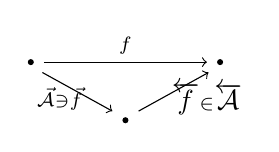
\begin{tikzpicture}[x=1.9em,y=1.5em]
  \fill (0,1.4) circle (1.1pt);
  \fill (3.6,1.4) circle (1.1pt);
  \fill (1.8,0) circle (1.1pt);
  \draw[->] (0.25,1.4) -- (3.35,1.4);
  \node at (1.8,1.8) {$\scriptstyle f$};
  \draw[->] (0.22,1.15) -- (1.55,0.22);
  \node at (0.55,0.52) {$\scriptstyle\rvAinc\ni\vec{f}$};
  \draw[->] (2.05,0.22) -- (3.38,1.15);
  \node at (3.35,0.52) {$\scriptstyle\overleftarrow{f}\in\rvAdec$};
\end{tikzpicture}
\end{rveq}
\end{enumerate}
\end{definition}

公理 (i) 蕴含 $\rvAinc\cap\rvAdec=\mathrm{obj}(\mathcal{A})$，而这两条条件
合在一起则蕴含 $\mathcal{A}$ 不含非恒同的自同构（见\cref{ex:reedy-isomorphism-identity}）。

\begin{example}\label{exa:inverse-category-reedy}
任何逆范畴 $\mathcal{J}$（见\cref{def:inverse-category}）都是一个 Reedy 范畴，
此时取 $\vec{\mathcal{J}}=\mathcal{J}$ 而 $\overleftarrow{\mathcal{J}}=\mathrm{obj}\mathcal{J}$。
反之，任何满足 $\mathcal{A}=\rvAinc$ 的 Reedy 范畴 $\mathcal{A}$ 都是一个逆
范畴，在此情形下，其度\emph{函数}可扩充为一个反映恒同箭头的度\emph{函子}。
\end{example}

\begin{example}\label{exa:delta-plus-reedy}
\trCategory{} $\boldsymbol{\Delta}_+$ 是一个 Reedy 范畴，其中取
$\vec{\boldsymbol{\Delta}}_+$ 为\trMonomorphism{}组成的子范畴、取
$\overleftarrow{\boldsymbol{\Delta}}_+$ 为\trEpimorphism{}组成的子范畴。在此，
方便的做法是利用序同构 $\mathbb{1}+\omega\cong\omega$ 来定义 $\mathrm{deg}[n]:=n$。
子范畴 $\boldsymbol{\Delta}$、$\boldsymbol{\Delta}_\top$ 与
$\boldsymbol{\Delta}_\bot$ 都继承类似的 Reedy 范畴结构。
\end{example}

\begin{remark}\label{rem:opposite-reedy}
若 $\mathcal{A}$ 是一个 Reedy 范畴，则 $\mathcal{A}^{\mathrm{op}}$ 亦是：其
Reedy 结构拥有同一度函数，但升度箭头与降度箭头互换。特别地，%
\cref{exa:inverse-category-reedy} 中的诸 Reedy 范畴对偶地定义了\textbf{正范畴}
（direct categories），后者配有反映恒同箭头的\trFunctor{}
$\mathrm{deg}\colon\mathcal{A}\to\omega$。
\end{remark}

\begin{example}\label{exa:product-reedy}
若 $\mathcal{A}$ 与 $\mathcal{B}$ 是 Reedy 范畴，则 $\mathcal{A}\times\mathcal{B}$
亦是，其度数为 $\mathrm{deg}(a,b):=\mathrm{deg}(a)+\mathrm{deg}(b)$
（见\cref{ex:product-reedy-category}）。
\end{example}

在本节余下的部分中，我们固定一个 Reedy 范畴 $\mathcal{A}$。我们把唯一分解
\eqref{eq:reedy-factorization} 称作映射 $f$ 的\textbf{Reedy 分解}（Reedy
factorization），并把对象 $\mathrm{cod}\,\vec{f}=\mathrm{dom}\,\overleftarrow{f}$
的度数称作 $f$ 的\textbf{度数}（degree）。我们的下一个目标是证明：
\begin{enumerate}[label=(\roman*)]
\item $f$ 的度数是 $f$ 可经由之分解的对象的最小度数。
\item $f$ 经由具有这一度数的对象之分解唯有 Reedy 分解。
\end{enumerate}

为证明这些论断，试考虑范畴
$\mathcal{F}act f:=(a/\mathcal{A})_{/f}\cong f/(\mathcal{A}_{/b})$，
其对象为 $f$ 的分解 $a\xrightarrow{\ g\ }c\xrightarrow{\ h\ }b$，其态射
$h\cdot g\to h'\cdot g'$ 是使得前侧三角形
\begin{center}
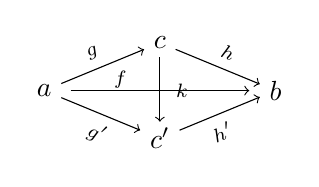
\begin{tikzpicture}[x=1.9em,y=1.5em]
  \node (c) at (2.2,2.3) {$c$};
  \node (a) at (0,1.15) {$a$};
  \node (b) at (4.4,1.15) {$b$};
  \node (c2) at (2.2,0) {$c'$};
  \draw[->] (a) -- (c) node[pos=0.45,above,sloped]{$\scriptstyle g$};
  \draw[->] (c) -- (b) node[pos=0.55,above,sloped]{$\scriptstyle h$};
  \draw[->] (0.5,1.15) -- (3.9,1.15);
  \node at (1.45,1.42) {$\scriptstyle f$};
  \draw[->] (2.2,1.95) -- (2.2,0.4);
  \node at (2.62,1.15) {$\scriptstyle k$};
  \draw[->] (a) -- (c2) node[pos=0.55,below,sloped]{$\scriptstyle g'$};
  \draw[->] (c2) -- (b) node[pos=0.45,below,sloped]{$\scriptstyle h'$};
\end{tikzpicture}
\end{center}
得以交换的映射 $k\colon c\to c'$。记
$\mathcal{F}act_{\leq n}f\subset\mathcal{F}act f$ 为经由度数至多为 $n$ 的对象
之分解所组成的全子范畴。

\begin{lemma}\label{lem:fact-connected}
范畴 $\mathcal{F}act f$ 是连通的，且每个全子范畴
$\mathcal{F}act_{\leq n}f$ 要么为空要么连通。使 $\mathcal{F}act_{\leq n}f$
非空的最小 $n$ 即 $f$ 的度数，并且
$\mathcal{F}act_{\leq\mathrm{deg}(f)}f\cong\mathbb{1}$。
\end{lemma}

\begin{proof}
考察 $h\cdot g\in\mathcal{F}act f$ 及其诸 Reedy 分解：
\begin{rveq}\label{eq:fact-zigzag}
\begin{tikzpicture}[x=2.0em,y=1.7em]
  \fill (0,2.6) circle (1.1pt);
  \fill (3.0,2.6) circle (1.1pt);
  \fill (6.0,2.6) circle (1.1pt);
  \fill (1.5,1.3) circle (1.1pt);
  \fill (4.5,1.3) circle (1.1pt);
  \fill (3.0,0) circle (1.1pt);
  \draw[->] (0.25,2.6) -- (2.75,2.6);
  \node at (1.5,2.98) {$\scriptstyle g$};
  \draw[->] (3.25,2.6) -- (5.75,2.6);
  \node at (4.5,2.98) {$\scriptstyle h$};
  \draw[->] (0.16,2.36) -- (1.3,1.52);
  \node at (0.3,1.78) {$\scriptstyle\vec{g}$};
  \draw[->] (1.72,1.52) -- (2.84,2.36);
  \node at (2.32,1.86) {$\scriptstyle\overleftarrow{g}$};
  \draw[->] (3.16,2.36) -- (4.3,1.52);
  \node at (3.7,1.86) {$\scriptstyle\vec{h}$};
  \draw[->] (4.7,1.52) -- (5.84,2.36);
  \node at (5.72,1.78) {$\scriptstyle\overleftarrow{h}$};
  \draw[->] (1.75,1.3) -- (4.25,1.3);
  \node at (3.0,0.92) {$\scriptstyle k=\vec{h}\cdot\overleftarrow{g}$};
  \draw[->] (1.64,1.1) -- (2.82,0.2);
  \node at (1.42,0.5) {$\scriptstyle\vec{k}$};
  \draw[->] (3.18,0.2) -- (4.36,1.1);
  \node at (4.62,0.5) {$\scriptstyle\overleftarrow{k}$};
\end{tikzpicture}
\end{rveq}
这样，我们便在 $\mathcal{F}act f$ 中定义了一条连接 $h\cdot g$ 与
$\overleftarrow{h}\,\overleftarrow{k}\cdot\vec{k}\,\vec{g}$ 的态射之字形链，
而由公理 (ii)，后者必为 $f$ 的 Reedy 分解。这表明 $\mathcal{F}act f$ 是连通的。

此外，公理 (i) 蕴含 $\mathrm{cod}(g)=\mathrm{dom}(h)$ 的度数至少是 $f$ 的
度数。特别地，若 $h\cdot g\in\mathcal{F}act_{\leq n}f$，则
\eqref{eq:fact-zigzag} 中的每个分解亦然，这就证明了 $\mathcal{F}act_{\leq n}f$
在非空时必定连通。这一图式还表明：每个非空范畴 $\mathcal{F}act_{\leq n}f$
都包含 Reedy 分解。于是，使之非空的最小 $n$ 便是 $f$ 的度数。

最后，若 $\mathrm{cod}(g)=\mathrm{dom}(h)$ 的度数等于 $f$ 的度数，则
$\overleftarrow{g}$ 与 $\vec{h}$（以及 $\vec{k}$ 与 $\overleftarrow{k}$）必为
恒同，由此我们推得 $g\in\rvAinc$ 且 $h\in\rvAdec$；也就是说，$h\cdot g$ 就是
Reedy 分解。于是，正如所断言的，
$\mathcal{F}act_{\leq\mathrm{deg}(f)}f\cong\mathbb{1}$ 是\trTerminal{}范畴。
\end{proof}

\cref{lem:fact-connected} 将被用来为 hom 双函子确立一种「胞腔分解」（cellular
decomposition）；这一 hom 双函子在别处记作 $\mathcal{A}(-,-)$，而在此处则
缩记为 $\mathcal{A}\in\mathcal{S}et^{\mathcal{A}^{\mathrm{op}}\times\mathcal{A}}$。
Reedy 结构使我们得以把双函子 $\mathcal{A}$ 呈现为\cref{def:cell-complex} 意义下
的一个胞腔复形，即一个由具有特定形状的基本「\trCell{}」之余积的推出构成的序列
复合。\cref{lem:fact-connected} 蕴含：度数至多为 $n$ 的箭头组成的子集可以
组装成 hom 双函子的一个\emph{子函子}。

\begin{definition}[hom 双函子的 $n$-骨架]\label{def:n-skeleton-hom-bifunctor}
对任何 Reedy 范畴 $\mathcal{A}$，\textbf{$n$-骨架}（$n$-skeleton）是度数至多
为 $n$ 的箭头组成的子函子
\[ \mathrm{sk}_n\mathcal{A}\hookrightarrow\mathcal{A}
   \in\mathcal{S}et^{\mathcal{A}^{\mathrm{op}}\times\mathcal{A}} \]
\end{definition}

存在显然的包含 $\mathrm{sk}_{n-1}\mathcal{A}\hookrightarrow\mathrm{sk}_n\mathcal{A}$。
序列
\[ \varnothing\hookrightarrow\mathrm{sk}_0\mathcal{A}\hookrightarrow\cdots
   \hookrightarrow\mathrm{sk}_{n-1}\mathcal{A}\hookrightarrow\mathrm{sk}_n\mathcal{A}
   \hookrightarrow\cdots\hookrightarrow\wcolim\mathrm{sk}_n\mathcal{A}\cong\mathcal{A} \]
的余极限就是 hom 双函子 $\mathcal{A}$。度数为 $n$ 的态射首次出现于
$\mathrm{sk}_n\mathcal{A}$ 中。剩下的工作是把每个包含
$\mathrm{sk}_{n-1}\mathcal{A}\hookrightarrow\mathrm{sk}_n\mathcal{A}$ 表述为
基本「\trCell{}」之余积的一个推出，这种基本「\trCell{}」我们即刻描述。

外部（逐点）积定义了一个双函子
$\square\colon\mathcal{S}et^{\mathcal{A}}\times\mathcal{S}et^{\mathcal{A}^{\mathrm{op}}}\to\mathcal{S}et^{\mathcal{A}^{\mathrm{op}}\times\mathcal{A}}$。对任何
$a\in\mathcal{A}$，都存在一个自然的「复合」映射
$\circ\colon\mathcal{A}_a\square\mathcal{A}^{a}\to\mathcal{A}$，其定义域是反变
可表示函子 $\mathcal{A}^{a}$ 与协变可表示函子 $\mathcal{A}_a$ 的外部积；此处
我们以 $\mathcal{A}^{a}$ 缩记 $\mathcal{A}(-,a)$、以 $\mathcal{A}_a$ 缩记
$\mathcal{A}(a,-)$。由\cref{lem:fact-connected}，经由一个度数为 $n$ 的对象 $a$
而分解的任何一对映射的复合都落于 $\mathrm{sk}_n\mathcal{A}$ 中，这就定义了
一个映射：
\[ \coprod_{\mathrm{deg}(a)=n}\mathcal{A}_a\square\mathcal{A}^{a}
   \xrightarrow{\ \circ\ }\mathrm{sk}_n\mathcal{A} \]

我们的下一项任务是描述定义域中经由
$\mathrm{sk}_{n-1}\mathcal{A}\hookrightarrow\mathrm{sk}_n\mathcal{A}$ 而分解的
那个子函子；为此我们需要一些新记号。

\begin{definition}[可表示函子的边缘]\label{def:boundary-representables}
若 $a\in\mathcal{A}$ 的度数为 $n$，则写作
\[ \begin{gathered}
\partial\mathcal{A}_a:=\mathrm{sk}_{n-1}\mathcal{A}_a
   \qquad\in\mathcal{S}et^{\mathcal{A}}\qquad\text{以及}\\
\partial\mathcal{A}^{a}:=\mathrm{sk}_{n-1}\mathcal{A}^{a}
   \qquad\in\mathcal{S}et^{\mathcal{A}^{\mathrm{op}}}.
\end{gathered} \]
\end{definition}

由\cref{lem:fact-connected}，$\partial\mathcal{A}_a\hookrightarrow\mathcal{A}_a$
是 $\mathcal{A}$ 中定义域为 $a$ 且\emph{不}居于 $\rvAinc$ 的箭头组成的子函子，
而 $\partial\mathcal{A}^{a}\hookrightarrow\mathcal{A}^{a}$ 是陪域为 $a$
且\emph{不}居于 $\rvAdec$ 的箭头组成的子函子。

特别地，外部\trLeibnizProduct
\[ \mathcal{A}_a\square\partial\mathcal{A}^{a}
   \cup_{\partial\mathcal{A}_a\square\partial\mathcal{A}^{a}}
   \partial\mathcal{A}_a\square\mathcal{A}^{a}
   \xhookrightarrow{\ (\partial\mathcal{A}_a\hookrightarrow\mathcal{A}_a)
   \mathbin{\widehat{\square}}(\partial\mathcal{A}^{a}\hookrightarrow\mathcal{A}^{a})\ }
   \mathcal{A}_a\square\mathcal{A}^{a} \]
定义了由满足 $\mathrm{dom}\,h=\mathrm{cod}\,g=a$ 的态射对 $h\cdot g$ 组成的
子函子，其中态射 $g$ 与 $h$ 至少有一个的度数小于 $a$ 的度数。

\begin{proposition}\label{prop:sk-square-pullback-pushout}
所展示的交换方块在 $\mathcal{S}et^{\mathcal{A}^{\mathrm{op}}\times\mathcal{A}}$
中既是一个拉回又是一个推出。
\begin{rveq}\label{eq:sk-square}
\begin{tikzpicture}[x=1.7em,y=1.6em]
  \node (TL) at (0,1.55) {$\displaystyle\coprod_{\mathrm{deg}(a)=n}\partial\mathcal{A}_a\square\mathcal{A}^{a}\cup\mathcal{A}_a\square\partial\mathcal{A}^{a}$};
  \node (TR) at (8.6,1.55) {$\displaystyle\coprod_{\mathrm{deg}(a)=n}\mathcal{A}_a\square\mathcal{A}^{a}$};
  \node (BL) at (0,0) {$\mathrm{sk}_{n-1}\mathcal{A}$};
  \node (BR) at (8.6,0) {$\mathrm{sk}_n\mathcal{A}$};
  \draw[right hook->] (TL) -- (TR);
  \draw[->] (0,1.1) -- (0,0.42);
  \node at (0.42,0.76) {$\scriptstyle\circ$};
  \draw[->] (8.6,1.1) -- (8.6,0.42);
  \node at (9.02,0.76) {$\scriptstyle\circ$};
  \draw[->] (BL) -- (BR);
\end{tikzpicture}
\end{rveq}
\end{proposition}

\eqref{eq:sk-square} 是拉回这一事实，将被用来便利其亦为推出之证明。

\begin{proof}
该拉回中的一个元素由 $f\in\mathrm{sk}_{n-1}\mathcal{A}$ 连同 $f=h\cdot g$
经由一个度数为 $n$ 的对象 $a$ 的一个分解构成。若 $h$ 与 $g$ 二者的度数都是
$n$，则\cref{lem:fact-connected} 告诉我们 $h\cdot g$ 是一个 Reedy 分解，这与
$f$ 的度数至多为 $n-1$ 的事实相矛盾。所以我们必有 $h\in\partial\mathcal{A}_a$
或 $g\in\partial\mathcal{A}^{a}$，这就告诉我们：从 \eqref{eq:sk-square} 左上角
出发的映射满映到该拉回上。由于顶行的水平映射是单的，该比较映射因而是一个
同构；也就是说，\eqref{eq:sk-square} 是一个拉回方块。

为证它是推出，现在只需证明右侧的竖直映射在
$\mathrm{sk}_{n-1}\mathcal{A}\hookrightarrow\mathrm{sk}_n\mathcal{A}$ 的补上是
一对一的。这由\cref{lem:fact-connected} 得出，后者论证了任何度数为 $n$ 的态射
都拥有经由该度数之对象的一个唯一分解，即其 Reedy 分解。
\end{proof}

作为\cref{prop:sk-square-pullback-pushout} 的推论，hom 双函子 $\mathcal{A}$
容有一个作为胞腔复形的典范呈现。

\begin{theorem}\label{thm:canonical-cell-complex}
包含 $\varnothing\hookrightarrow\mathcal{A}\in\mathcal{S}et^{\mathcal{A}^{\mathrm{op}}\times\mathcal{A}}$ 拥有一个作为胞腔
复形的典范呈现：
\begin{center}
\begin{tikzpicture}[x=1.25em,y=1.6em]
  \node (TL) at (0,1.7) {$\displaystyle\coprod_{\mathrm{deg}(a)=n}\partial\mathcal{A}_a\square\mathcal{A}^{a}\cup\mathcal{A}_a\square\partial\mathcal{A}^{a}$};
  \node (TR) at (8.8,1.7) {$\displaystyle\coprod_{\mathrm{deg}(a)=n}\mathcal{A}_a\square\mathcal{A}^{a}$};
  \draw[right hook->] (TL) -- (TR);
  \draw[->] (0,1.22) -- (0,0.5);
  \node at (0.4,0.86) {$\scriptstyle\circ$};
  \draw[->] (8.8,1.22) -- (8.8,0.5);
  \node at (9.2,0.86) {$\scriptstyle\circ$};
  \node (E) at (-9.6,0) {$\varnothing$};
  \node (S0) at (-7.2,0) {$\mathrm{sk}_0\mathcal{A}$};
  \node (D1) at (-5.0,0) {$\cdots$};
  \node (BL) at (0,0) {$\mathrm{sk}_{n-1}\mathcal{A}$};
  \node (BR) at (8.8,0) {$\mathrm{sk}_n\mathcal{A}$};
  \node (D2) at (10.9,0) {$\cdots$};
  \node (CL) at (14.6,0) {$\wcolim_n\mathrm{sk}_n\mathcal{A}\cong\mathcal{A}$};
  \draw[right hook->] (-9.2,0) -- (-8.3,0);
  \draw[dotted,->] (-6.1,0) -- (-5.55,0);
  \draw[dotted,->] (-4.45,0) -- (-1.8,0);
  \draw[right hook->] (1.2,0) -- (7.9,0);
  \node at (8.15,0.34) {$\scriptstyle\lrcorner$};
  \draw[dotted,->] (9.7,0) -- (10.35,0);
  \draw[->] (11.5,0) -- (11.9,0);
\end{tikzpicture}
\end{center}
也就是说，它是诸\trCell{}之余积的推出的一个序列复合，而诸\trCell{}定义为
外部\trLeibnizProduct
\[ (\partial\mathcal{A}_a\hookrightarrow\mathcal{A}_a)\mathbin{\widehat{\square}}
   (\partial\mathcal{A}^{a}\hookrightarrow\mathcal{A}^{a}), \]
其中 $\mathcal{A}$ 的每个度数为 $n$ 的对象 $a$ 所对应的\trCell{}在第 $n$
阶段粘合。
\end{theorem}

作为\cref{thm:canonical-cell-complex} 的推论，任何态射
$f\in\mathcal{M}^{\mathcal{A}}$ 自身就是一个胞腔复形：$\mathcal{A}$ 的胞腔
分解经由取加权余极限而被转译为 $f$ 的一个胞腔分解。若改为取加权极限，则把
$\mathcal{A}$ 的胞腔分解转变为 $f$ 的一个「Postnikov 呈现」（Postnikov
presentation）——即作为可数塔之极限的、由特定映射之积的拉回构成的一座塔。
这类结果正是 \cite{bib107} 那句口号——「一切尽在权重之中」——的范例。在证明
这一推论之前，我们需要一些记号，以记写作为基本\trCell{}与基本层登场的那些映射。

\begin{definition}[锁存对象与匹配对象]\label{def:latching-matching-objects}
设 $a\in\mathcal{A}$。\trDiagram{} $X\in\mathcal{M}^{\mathcal{A}}$ 在 $a$ 处的
\textbf{锁存对象}（latching object）与\textbf{匹配对象}分别定义为以适当变式的
边缘可表示函子加权所得的余极限与极限：
\[ L^{a}X:=\wcolim_{\partial\mathcal{A}^{a}}X\qquad
   M^{a}X:=\wlim_{\partial\mathcal{A}_a}X. \]
\end{definition}

边缘包含 $\partial\mathcal{A}^{a}\hookrightarrow\mathcal{A}^{a}$ 与
$\partial\mathcal{A}_a\hookrightarrow\mathcal{A}_a$ 诱导出\textbf{\trLatchingMap}
（latching map）与\textbf{匹配映射} $\ell^{a}\colon L^{a}X\to X^{a}$ 与
$m^{a}\colon X^{a}\to M^{a}X$，其依据是附录 A 中的%
\cref{def:weighted-limit-colimit-axiomatic}(i) 的诸同构
$\wcolim_{\mathcal{A}^{a}}X\cong X^{a}\cong\wlim_{\mathcal{A}_a}X$。

\begin{definition}[相对锁存映射与相对匹配映射]\label{def:relative-latching-matching-maps}
自然变换 $f\colon X\to Y\in\mathcal{M}^{\mathcal{A}}$ 的\textbf{相对锁存映射}
（relative latching map）与\textbf{相对匹配映射}定义为 Leibniz 加权余极限与
加权极限
\[ \hat{\ell}^{a}f:=\widehat{\wcolim}_{\partial\mathcal{A}^{a}\hookrightarrow\mathcal{A}^{a}}f
   \qquad
   \hat{m}^{a}f:=\widehat{\wlim}_{\partial\mathcal{A}_a\hookrightarrow\mathcal{A}_a}f, \]
亦即由下列诸拉回与诸推出给出：
\begin{center}
\begin{tikzpicture}[x=2.1em,y=1.7em]
  \node (LX) at (0,2.4) {$L^{a}X$};
  \node (Xa) at (3.2,2.4) {$X^{a}$};
  \node (LY) at (0,1.0) {$L^{a}Y$};
  \fill (1.9,1.0) circle (1.1pt);
  \node (Ya) at (4.4,0.2) {$Y^{a}$};
  \draw[->] (LX) -- (Xa) node[midway,above]{$\scriptstyle\ell^{a}$};
  \draw[->] (0,2.05) -- (0,1.35) node[midway,left]{$\scriptstyle L^{a}f$};
  \draw[->] (0.55,1.0) -- (1.55,1.0);
  \node at (2.42,1.32) {$\scriptstyle\lrcorner$};
  \draw[dashed,->] (2.18,0.86) to[bend right=12] node[pos=0.5,above]{$\scriptstyle\hat{\ell}^{a}f$} (4.05,0.35);
  \draw[->] (Xa) to[bend left=22] node[pos=0.5,above]{$\scriptstyle f^{a}$} (Ya);
  \draw[->] (LY) to[bend right=15] node[pos=0.5,below]{$\scriptstyle\ell^{a}$} (Ya);
\end{tikzpicture}
\qquad
\begin{tikzpicture}[x=2.1em,y=1.7em]
  \node (Xa) at (0,2.4) {$X^{a}$};
  \node (MX) at (3.4,2.4) {$M^{a}X$};
  \fill (1.5,1.15) circle (1.1pt);
  \node (Ya) at (0,0.2) {$Y^{a}$};
  \node (MY) at (3.4,0.2) {$M^{a}Y$};
  \draw[->] (Xa) -- (MX) node[midway,above]{$\scriptstyle m^{a}$};
  \draw[dashed,->] (0.3,2.05) -- (1.25,1.32) node[pos=0.45,left]{$\scriptstyle\hat{m}^{a}f$};
  \draw[->] (1.78,1.3) -- (2.95,2.1);
  \node at (2.12,0.98) {$\scriptstyle\lrcorner$};
  \draw[->] (1.22,1.02) -- (0.32,0.42);
  \draw[->] (MX) -- (MY) node[midway,right]{$\scriptstyle M^{a}f$};
  \draw[->] (Ya) -- (MY) node[midway,below]{$\scriptstyle m^{a}$};
  \draw[->] (Xa) to[bend right=22] node[pos=0.5,left]{$\scriptstyle f^{a}$} (Ya);
\end{tikzpicture}
\end{center}
其中的映射为 $L^{a}f:=\wcolim_{\partial\mathcal{A}^{a}}f$ 与
$M^{a}f:=\wlim_{\partial\mathcal{A}_a}f$。
\end{definition}

\begin{notation}\label{not:sk-cosk-diagrams}
对任何\trDiagram{} $X\in\mathcal{M}^{\mathcal{A}}$，记
\[ \mathrm{sk}_nX:=\wcolim_{\mathrm{sk}_n\mathcal{A}}X\qquad\text{以及}\qquad
   \mathrm{cosk}_nX:=\wlim_{\mathrm{sk}_n\mathcal{A}}X \]
为把附录 A 中的\cref{ex:enriched-profunctor-weights} 的加权余极限与加权极限
双函子
\[ \wcolim_{--}\colon\mathcal{S}et^{\mathcal{A}^{\mathrm{op}}\times\mathcal{A}}
   \times\mathcal{M}^{\mathcal{A}}\to\mathcal{M}^{\mathcal{A}}
   \qquad\text{与}\qquad
   \wlim_{--}\colon(\mathcal{S}et^{\mathcal{A}^{\mathrm{op}}\times\mathcal{A}})^{\mathrm{op}}
   \times\mathcal{M}^{\mathcal{A}}\to\mathcal{M}^{\mathcal{A}} \]
施加于带权 $\mathrm{sk}_n\mathcal{A}$ 的\trDiagram{} $X$ 所得的结果。
\end{notation}

回顾为带余积与积的\trCategory{}所定义的集合张量
$\ast\colon\mathcal{S}et\times\mathcal{M}\to\mathcal{M}$ 与集合余张量
$\{,\}\colon\mathcal{S}et^{\mathrm{op}}\times\mathcal{M}\to\mathcal{M}$ 这两个%
\trBifunctor。

\begin{corollary}\label{cor:morphism-cell-complex}
设 $\mathcal{A}$ 是一个 Reedy 范畴，并设 $\mathcal{M}$ 完备且余完备。任何
态射 $f\colon X\to Y\in\mathcal{M}^{\mathcal{A}}$ 都是一个胞腔复形
\[ X\to
   X\cup_{\mathrm{sk}_0X}\mathrm{sk}_0Y\to\cdots\to
   X\cup_{\mathrm{sk}_{n-1}X}\mathrm{sk}_{n-1}Y\to
   X\cup_{\mathrm{sk}_nX}\mathrm{sk}_nY\to\cdots\to
   \wcolim\cong Y \]
其第 $n$ 阶段粘合以度数为 $n$ 的诸对象 $a$ 为标的诸\trCell
\[ (\partial\mathcal{A}_a\hookrightarrow\mathcal{A}_a)\mathbin{\widehat{\ast}}
   \hat{\ell}^{a}f \]
的余积，并且也是一座「Postnikov 塔」（Postnikov tower）
\[ \begin{gathered}
X\cong\lim\to\cdots\to
\mathrm{cosk}_nX\times_{\mathrm{cosk}_nY}Y\to\\
\mathrm{cosk}_{n-1}X\times_{\mathrm{cosk}_{n-1}Y}Y\to\cdots\to
\mathrm{cosk}_0X\times_{\mathrm{cosk}_0Y}Y\to Y
\end{gathered} \]
其第 $n$ 层是以度数为 $n$ 的诸对象 $a$ 为标的诸映射
\[ \{\partial\mathcal{A}^{a}\hookrightarrow\mathcal{A}^{a},\ \hat{m}^{a}f\} \]
之积。
\end{corollary}

\begin{proof}
这一对对偶结果可立即得到：只需把附录 A 中的\cref{ex:enriched-profunctor-weights}
的加权余极限与加权极限双函子
\[ \wcolim_{--}\colon\mathcal{S}et^{\mathcal{A}^{\mathrm{op}}\times\mathcal{A}}
   \times\mathcal{M}^{\mathcal{A}}\to\mathcal{M}^{\mathcal{A}}
   \qquad\text{以及}\qquad
   \wlim_{--}\colon(\mathcal{S}et^{\mathcal{A}^{\mathrm{op}}\times\mathcal{A}})^{\mathrm{op}}
   \times\mathcal{M}^{\mathcal{A}}\to\mathcal{M}^{\mathcal{A}} \]
施加于\cref{thm:canonical-cell-complex} 的诸胞腔复形呈现即可；并回想附录 A 中
的\cref{def:weighted-limit-colimit-axiomatic}(ii)：这两个双函子在权上都是
余连续的。

为看出 $f$ 的胞腔复形呈现具有所断言的形状，注意：对任何\trDiagram{}
$X\in\mathcal{M}^{\mathcal{A}}$ 与由 $U\in\mathcal{S}et^{\mathcal{A}}$ 及
$V\in\mathcal{S}et^{\mathcal{A}^{\mathrm{op}}}$ 的外部积所定义的权，都存在一个
自然\trIsomorphism{} $\wcolim_{U\square V}X\cong U\ast\wcolim_{V}X$，它可扩充
为诸\trLeibnizProduct{}之间的一个自然\trIsomorphism
（\cref{prop:leibniz-construction-preserves}(i)）。

由余 Yoneda 引理（coYoneda lemma），
$f\cong\wcolim_{\mathcal{A}}f\cong\widehat{\wcolim}_{\varnothing\hookrightarrow\mathcal{A}}f$。
由\cref{prop:leibniz-construction-preserves}(vii)，Leibniz 加权余极限函子
$\wcolim_{-}f$ 保持胞腔结构。于是，$f$ 容有一个作为胞腔复形的典范呈现，其诸%
\trCell{}为
\[ \widehat{\wcolim}_{(\partial\mathcal{A}_a\hookrightarrow\mathcal{A}_a)
   \mathbin{\widehat{\square}}(\partial\mathcal{A}^{a}\hookrightarrow\mathcal{A}^{a})}f
   \cong(\partial\mathcal{A}_a\hookrightarrow\mathcal{A}_a)\mathbin{\widehat{\ast}}
   \widehat{\wcolim}_{\partial\mathcal{A}^{a}\hookrightarrow\mathcal{A}^{a}}f
   \cong(\partial\mathcal{A}_a\hookrightarrow\mathcal{A}_a)\mathbin{\widehat{\ast}}
   \hat{\ell}^{a}f. \]
\end{proof}

这一呈现对 Reedy 范畴 $\boldsymbol{\Delta}^{\mathrm{op}}$ 而言最为眼熟。此处
我们以 $\boldsymbol{\Delta}^{n}$ 表示标准 $n$-\trSimplex{} $\Delta[n]$、以
$\partial\boldsymbol{\Delta}^{n}$ 表示其边缘——这些是文献中通行的记号约定，
且与\cref{def:boundary-representables} 的记法相容。

\begin{example}\label{exa:skeletal-filtration}
取值于任何余完备\trCategory{}的单纯对象 $Y$ 容有一个骨架过滤
（skeletal filtration）
\[ \varnothing\to\mathrm{sk}_0Y\to\cdots\to
   \mathrm{sk}_{n-1}Y\to\mathrm{sk}_nY\to\cdots\to
   \wcolim_n\mathrm{sk}_nY\cong Y \]
其中从阶段 $n-1$ 到阶段 $n$ 的一步由一个推出给出
\begin{center}
\begin{tikzpicture}[x=2.0em,y=1.5em]
  \node (TL) at (0,1.6) {$\boldsymbol{\Delta}^{n}\ast L_nY\cup\partial\boldsymbol{\Delta}^{n}\ast Y_n$};
  \node (TR) at (6.8,1.6) {$\boldsymbol{\Delta}^{n}\ast Y_n$};
  \node (BL) at (0,0) {$\mathrm{sk}_{n-1}Y$};
  \node (BR) at (6.8,0) {$\mathrm{sk}_nY$};
  \draw[->] (TL) -- (TR);
  \draw[->] (0,1.2) -- (0,0.42);
  \draw[->] (6.8,1.2) -- (6.8,0.42);
  \draw[->] (BL) -- (BR);
  \node at (6.15,0.36) {$\scriptstyle\lrcorner$};
\end{tikzpicture}
\end{center}
其中 $L_nY\to Y_n$ 是「退化 $n$-单纯形」组成的对象。

把\trYonedaEmbedding{}视作一个单纯对象
$\boldsymbol{\Delta}\in(\mathcal{S}et^{\boldsymbol{\Delta}})^{\boldsymbol{\Delta}^{\mathrm{op}}}$，
上式便特化为\cref{thm:canonical-cell-complex} 的那个 hom 双函子的「典范胞腔
复形呈现」
\begin{center}
\begin{tikzpicture}[x=1.6em,y=1.5em]
  \node (TL) at (0,1.7) {$\boldsymbol{\Delta}^{n}\times\partial\boldsymbol{\Delta}_n\cup\partial\boldsymbol{\Delta}^{n}\times\boldsymbol{\Delta}_n$};
  \node (TR) at (6.2,1.7) {$\boldsymbol{\Delta}^{n}\times\boldsymbol{\Delta}_n$};
  \draw[right hook->] (TL) -- (TR);
  \draw[->] (0,1.28) -- (0,0.5);
  \draw[->] (6.2,1.28) -- (6.2,0.5);
  \node (E) at (-6.0,0) {$\varnothing$};
  \node (D1) at (-4.4,0) {$\cdots$};
  \node (BL) at (0,0) {$\mathrm{sk}_{n-1}\boldsymbol{\Delta}$};
  \node (BR) at (6.2,0) {$\mathrm{sk}_n\boldsymbol{\Delta}$};
  \node (D2) at (8.3,0) {$\cdots$};
  \node (DT) at (10.3,0) {$\boldsymbol{\Delta}$};
  \draw[right hook->] (-5.5,0) -- (-4.95,0);
  \draw[right hook->] (-3.9,0) -- (-1.6,0);
  \draw[right hook->] (1.15,0) -- (5.1,0);
  \node at (5.5,0.36) {$\scriptstyle\lrcorner$};
  \draw[right hook->] (7.3,0) -- (7.75,0);
  \draw[right hook->] (8.85,0) -- (9.9,0);
\end{tikzpicture}
\end{center}
\end{example}

总而言之，\cref{cor:morphism-cell-complex} 告诉我们：取值于完备且余完备%
\trCategory{}的、形状为 $\mathcal{A}$ 的图表之间的一个一般的%
\trNaturalTransformation，可以被表达为
\begin{enumerate}[label=(\roman*)]
\item 一个胞腔复形，其诸\trCell{}是由协变可表示函子的边缘包含与相对锁存映射
  构造的\trLeibnizTensor；并且对偶地
\item 作为一座 Postnikov 塔，其诸层是由反变可表示函子的边缘包含与相对匹配
  映射构造的\trLeibnizCotensor。
\end{enumerate}

这解释了这些映射之于 Reedy 范畴论的重要性，我们将在下一节中发现这一点。

\subsection*{练习}

\begin{exercise}\label{ex:reedy-isomorphism-identity}
证明：（严格的）Reedy 范畴中的任何\trIsomorphism{}都是恒同。
\end{exercise}

\begin{exercise}\label{ex:product-reedy-category}
证明：两个 Reedy 范畴的乘积是一个 Reedy 范畴，其中对象的度数取为诸度数
之和。
\end{exercise}

   %

\providecommand{\llsq}{\mathrel{\square}}%
\providecommand{\rvW}{\mathbf{W}}  %
\providecommand{\rvC}{\mathbf{C}}  %
\providecommand{\rvF}{\mathbf{F}}  %
\providecommand{\Cat}{\mathcal{C}at}%
\providecommand{\sSet}{s\mathcal{S}et}%
\providecommand{\wlim}{\operatorname{lim}}%
\providecommand{\wcolim}{\operatorname{colim}}%
\providecommand{\lan}{\operatorname{lan}}%
\providecommand{\ran}{\operatorname{ran}}%

\section{Reedy 模型结构}\label{sec:the-reedy-model-structure}

本节的目标在于说明：$\mathcal{M}$ 上的任何\trWeakFactorizationSystem{}如何
产生 $\mathcal{M}^{\mathcal{A}}$ 上的一个\emph{Reedy 弱分解系统}（Reedy weak
factorization system），进而说明：由 $\mathcal{M}$ 上一个\trModelStructure{}%
相伴的诸 Reedy 弱分解系统定义 $\mathcal{M}^{\mathcal{A}}$ 上的\emph{Reedy
\trModelStructure}。这两个结果都源自对「归纳地定义由 Reedy \trCategory{}标引
的\trFunctor{}与\trNaturalTransformation{}需要什么」所作的分析。最后，我们证
明加权\trLimit{}二函子与加权\trColimit{}二函子定义 Quillen \trBifunctor——这
是一个更一般的代数结果的重要特例——并讨论这一结果对由 Reedy \trCategory{}标引
的\trHomotopyLimit{}与\trHomotopyColimit{}理论的种种意涵。

这一工作需要一项准备：讨论上一节引入的诸骨架与诸余骨架如何在 Reedy 形状的%
\trDiagram{}的归纳定义中登场。对一个 Reedy \trCategory{} $\mathcal{A}$，记
\[
\mathcal{A}_{\le 0}\subset\mathcal{A}_{\le 1}\subset\cdots\subset
\mathcal{A}_{\le n-1}\subset\mathcal{A}_{\le n}\subset\cdots\subset\mathcal{A}
\]
为由度数至多为下标所示序数的对象组成的诸全子范畴。这些范畴为我们提供了一种
理解\cref{not:sk-cosk-diagrams}的\trSkeleton{}函子与余骨架函子的新方式。

\begin{lemma}\label{lem:kan-adjoint-triple}
对任何\trComplete{}且\trCocomplete{}的\trCategory{} $\mathcal{M}$，限制与
左、右\trKanExtension{}定义\trFunctor{}的一个\trAdjointTriple
\begin{center}
\begin{tikzpicture}[x=1.7em,y=1.4em]
  \node (M) at (0,0) {$\mathcal{M}^{\mathcal{A}}$};
  \node (Mn) at (5.0,0) {$\mathcal{M}^{\mathcal{A}_{\le n}}$};
  \draw[->] (0.7,0.42) .. controls (1.8,1.05) and (3.2,1.05) .. (4.3,0.42);
  \node at (2.5,1.12) {$\scriptstyle\lan_n$};
  \draw[->] (0.8,0) -- (4.2,0);
  \node at (2.5,0.32) {$\scriptstyle\mathrm{res}_n$};
  \node at (1.45,0.72) {$\scriptstyle\dashv$};
  \draw[->] (4.3,-0.42) .. controls (3.2,-1.05) and (1.8,-1.05) .. (0.7,-0.42);
  \node at (2.5,-1.12) {$\scriptstyle\ran_n$};
  \node at (1.45,-0.72) {$\scriptstyle\dashv$};
\end{tikzpicture}
\end{center}
其诱导的余单子 $\mathrm{sk}_n\coloneqq\lan_n\circ\mathrm{res}_n$ 与单子
$\mathrm{cosk}_n\coloneqq\ran_n\circ\mathrm{res}_n$ 相伴
$\mathrm{sk}_n\dashv\mathrm{cosk}_n$，且自然同构于由加权\trColimit{}与加权%
\trLimit{}所定义的函子
\[
\lan_n\mathrm{res}_n(-)\cong\wcolim_{\mathrm{sk}_n\mathcal{A}}-
\qquad\text{与}\qquad
\ran_n\mathrm{res}_n(-)\cong\wlim_{\mathrm{sk}_n\mathcal{A}}-.
\]
\end{lemma}
\begin{proof}
\cref{ex:prove-kan-adjoint-triple}。
\end{proof}

例如：

\begin{definition}\label{def:simplex-skeleton-coskeleton}
将上述记号特化，记 $\Delta_{\le n}\subset\Delta$ 为第 1 章中的%
\cref{not:simplex-category}的\trSimplexCategory{}中由序数
$[0],\ldots,[n]$ 张成的全子范畴。限制与左、右\trKanExtension{}定义伴随
\begin{center}
\begin{tikzpicture}[x=1.7em,y=1.4em]
  \node (S) at (0,0) {$\mathcal{S}et^{\Delta^{\mathrm{op}}}$};
  \node (T) at (5.6,0) {$\mathcal{S}et^{\Delta_{\le n}^{\mathrm{op}}}$};
  \draw[->] (0.9,0.42) .. controls (2.1,1.05) and (3.6,1.05) .. (4.7,0.42);
  \node at (2.8,1.12) {$\scriptstyle\lan_n$};
  \draw[->] (1.0,0) -- (4.6,0);
  \node at (2.8,0.32) {$\scriptstyle\mathrm{res}_n$};
  \node at (1.75,0.72) {$\scriptstyle\dashv$};
  \draw[->] (4.7,-0.42) .. controls (3.6,-1.05) and (2.1,-1.05) .. (0.9,-0.42);
  \node at (2.8,-1.12) {$\scriptstyle\ran_n$};
  \node at (1.75,-0.72) {$\scriptstyle\dashv$};
\end{tikzpicture}
\end{center}
其在 $\sSet$ 上诱导一个幂等余单子
$\mathrm{sk}_n\coloneqq\lan_n\circ\mathrm{res}_n$ 与一个幂等单子
$\mathrm{cosk}_n\coloneqq\ran_n\circ\mathrm{res}_n$，二者相伴
$\mathrm{sk}_n\dashv\mathrm{cosk}_n$。这一余单子与单子的余单位与单位定义诸%
典范映射
\[
\mathrm{sk}_n X\xrightarrow{\;\varepsilon\;}X\xrightarrow{\;\eta\;}
\mathrm{cosk}_n X
\]
把单纯集 $X$ 与其\textbf{$n$-\trSkeleton}（$n$-skeleton）及\textbf{$n$-余骨架}
（$n$-coskeleton）联系起来。若上述映射中的前者、相应地后者，是\trIsomorphism，
我们便说 $X$ 是\textbf{$n$-骨架的}（$n$-skeletal）或\textbf{$n$-余骨架的}
（$n$-coskeletal）。
\end{definition}
下述引理记录了由全忠实包含
$\mathrm{sk}_n\mathcal{A}\hookrightarrow\mathcal{A}$ 所产生的\trAdjointTriple{}
$\lan_n\dashv\mathrm{res}_n\dashv\ran_n$ 的若干特殊性质。特别地，从单纯集的
$n$-\trSkeleton{}到其 $n$-余骨架的\trCanonical{}映射可以在更一般的情形下定义，
而不只是对作为限制而定义的诸\trDiagram：

\begin{lemma}\label{lem:fully-faithful-adjoint-triple}
对任何\trFullyFaithful{}包含 $\mathcal{B}\hookrightarrow\mathcal{A}$ 与%
\trComplete{}且\trCocomplete{}的\trCategory{} $\mathcal{M}$，试考虑相伴的%
\trAdjointTriple：
\begin{center}
\begin{tikzpicture}[x=1.7em,y=1.4em]
  \node (M) at (0,0) {$\mathcal{M}^{\mathcal{A}}$};
  \node (Mb) at (5.0,0) {$\mathcal{M}^{\mathcal{B}}$};
  \draw[->] (0.7,0.42) .. controls (1.8,1.05) and (3.2,1.05) .. (4.3,0.42);
  \node at (2.5,1.12) {$\scriptstyle\lan$};
  \draw[->] (0.8,0) -- (4.2,0);
  \node at (2.5,0.32) {$\scriptstyle\mathrm{res}$};
  \node at (1.45,0.72) {$\scriptstyle\dashv$};
  \draw[->] (4.3,-0.42) .. controls (3.2,-1.05) and (1.8,-1.05) .. (0.7,-0.42);
  \node at (2.5,-1.12) {$\scriptstyle\ran$};
  \node at (1.45,-0.72) {$\scriptstyle\dashv$};
\end{tikzpicture}
\end{center}
\begin{enumerate}[label=(\roman*)]
\item 诸\trFunctor{} $\lan$，$\ran\colon\mathcal{M}^{\mathcal{B}}\to\mathcal{M}^{\mathcal{A}}$
  是\trFullyFaithful{}；也就是说，$\lan\dashv\mathrm{res}$ 的\trUnit{}%
  与 $\mathrm{res}\dashv\ran$ 的\trCounit{}是\trIsomorphism。
\item 下方交换方块中的公共复合定义一个\trCanonical{}\trNaturalTransformation
\begin{center}
\begin{tikzpicture}[x=2.0em,y=1.6em]
  \node (lan) at (0,1.3) {$\lan$};
  \node (rrl) at (4.6,1.3) {$\ran\,\mathrm{res}\,\lan$};
  \node (lrr) at (0,-1.1) {$\lan\,\mathrm{res}\,\ran$};
  \node (ran) at (4.6,-1.1) {$\ran$};
  \draw[double,->] (1.0,1.3) -- (3.1,1.3);
  \node at (2.05,1.66) {$\scriptstyle\eta\circ\lan$};
  \draw[double,->] (0,0.85) -- (0,-0.55);
  \node at (-1.3,0.15) {$\scriptstyle\lan\circ\varepsilon^{-1}$};
  \draw[double,->] (4.6,0.85) -- (4.6,-0.55);
  \node at (5.9,0.15) {$\scriptstyle\ran\circ\eta^{-1}$};
  \draw[double,->] (1.0,-1.1) -- (3.6,-1.1);
  \node at (2.3,-1.46) {$\scriptstyle\mathrm{coran}$};
  \draw[double,dashed,->] (0.35,1.0) -- (4.25,-0.85);
  \node at (2.7,0.42) {$\scriptstyle\tau$};
\end{tikzpicture}
\end{center}
\end{enumerate}
\end{lemma}

虽然我们觉得 (ii) 中的交换方块颇为有趣，但由于包含 $\mathcal{B}\hookrightarrow\mathcal{A}$
是全忠实的，$\tau$ 其实可以更简单地定义：利用左、右\trKanExtension{}的%
\trUniversalProperty，把它取作延拓给定图表的始\trFunctor{}与终\trFunctor。

\begin{proof}
众所周知：一支\trRightAdjoint{}\trFunctor{}是\trFullyFaithful{}，当且仅当
其余单位是\trIsomorphism；而且沿全忠实\trFunctor{}的\trPointwise{}右%
\trKanExtension{}之余单位是\trIsomorphism；至于证明，请把第 9 章中的%
\cref{lem:fully-faithful-characterizations}与\cref{prop:extensions-along-fully-faithful}
的结果特化到 ∞-宇宙 $\Cat$ 之上。这些陈述及其对偶证明了 (i)。

在 (ii) 中，$\tau$ 被定义为 $\eta^{-1}\colon\mathrm{res}\,\lan\Rightarrow\mathrm{id}$
在 $\mathrm{res}\dashv\ran$ 之下的伴随转置，同时也可被定义为
$\varepsilon^{-1}\colon\mathrm{id}\Rightarrow\mathrm{res}\,\ran$ 在
$\lan\dashv\mathrm{res}$ 之下的伴随转置。为见这两个定义相符，请注意：前者
断言下方右侧两个态射的复合是左侧态射的唯一右逆，而后者断言下方左侧两个态射
的复合是右侧态射的唯一左逆：
\[
\mathrm{id}\;\underset{\cong}{\xRightarrow{\;\eta\;}}\;
\mathrm{res}\,\lan\;\xRightarrow{\;\mathrm{res}\,\tau\;}\;
\mathrm{res}\,\ran\;\underset{\cong}{\xRightarrow{\;\varepsilon\;}}\;
\mathrm{id}
\]
换言之，两个定义都恰好断言：所示的三重复合是恒同。
\end{proof}

以这种方式，我们得到一个\trNaturalTransformation{}
$\tau_n\colon\mathrm{sk}_n\Rightarrow\mathrm{cosk}_n$，它介于\cref{lem:kan-adjoint-triple}
中引入的余单子与单子之间。这些结构使我们得以归纳地定义 Reedy \trDiagram：

\begin{proposition}[图表的归纳定义]\label{prop:inductive-definition-of-diagrams}
\begin{enumerate}[label=(\roman*)]
\item 一个\trDiagram{} $X\in\mathcal{M}^{\mathcal{A}_{\le n-1}}$ 连同对
  $\mathcal{A}$ 中每个度数为 $n$ 的对象 $a$ 的一族因子分解
\begin{center}
\begin{tikzpicture}[x=1.9em,y=1.5em]
  \node (sk) at (0,1.3) {$\mathrm{sk}_{n-1}X^{a}$};
  \node (ck) at (5.4,1.3) {$\mathrm{cosk}_{n-1}X^{a}$};
  \node (X) at (2.7,0) {$X^{a}$};
  \draw[->] (sk) to[bend left=15] node[above]{$\scriptstyle\tau_{n-1}X^{a}$} (ck);
  \draw[->,dashed] (0.55,1.0) -- (2.3,0.28) node[pos=0.5,below,sloped]{$\scriptstyle i^{a}$};
  \draw[->,dashed] (3.1,0.28) -- (4.9,1.0) node[pos=0.5,below,sloped]{$\scriptstyle p^{a}$};
\end{tikzpicture}
\end{center}
  唯一地确定 $X$ 到一个\trDiagram{} $X\in\mathcal{M}^{\mathcal{A}_{\le n}}$
  的扩张。
\item 一个\trNaturalTransformation{} $f\colon X\to Y\in\mathcal{M}^{\mathcal{A}_{\le n-1}}$
  连同对 $\mathcal{A}$ 中每个度数为 $n$
  的对象 $a$ 的一族因子分解
\begin{center}
\begin{tikzpicture}[x=1.9em,y=1.5em]
  \node (skX) at (0,2.4) {$\mathrm{sk}_{n-1}X^{a}$};
  \node (XX) at (3.0,2.4) {$X^{a}$};
  \node (ckX) at (6.0,2.4) {$\mathrm{cosk}_{n-1}X^{a}$};
  \node (skY) at (0,-0.5) {$\mathrm{sk}_{n-1}Y^{a}$};
  \node (YY) at (3.0,-0.5) {$Y^{a}$};
  \node (ckY) at (6.0,-0.5) {$\mathrm{cosk}_{n-1}Y^{a}$};
  \draw[->] (skX) to[bend left=14] node[above,pos=0.45]{$\scriptstyle\tau_{n-1}X^{a}$} (ckX);
  \draw[->,dashed] (skX) -- node[below,pos=0.6]{$\scriptstyle i^{a}$} (XX);
  \draw[->,dashed] (XX) -- node[below,pos=0.4]{$\scriptstyle p^{a}$} (ckX);
  \draw[->] (0,2.0) -- (0,-0.1) node[midway,left]{$\scriptstyle\mathrm{sk}_{n-1}f^{a}$};
  \draw[->,dashed] (3.0,2.05) -- (3.0,-0.15) node[pos=0.35,right]{$\scriptstyle f^{a}$};
  \draw[->] (6.0,2.05) -- (6.0,-0.15) node[midway,right]{$\scriptstyle\mathrm{cosk}_{n-1}f^{a}$};
  \draw[->,dashed] (skY) -- node[below,pos=0.6]{$\scriptstyle i^{a}$} (YY);
  \draw[->,dashed] (YY) -- node[below,pos=0.4]{$\scriptstyle p^{a}$} (ckY);
  \draw[->] (skY) to[bend right=14] node[below,pos=0.45]{$\scriptstyle\tau_{n-1}Y^{a}$} (ckY);
\end{tikzpicture}
\end{center}
  唯一地确定 $f$ 到一个映射 $f\colon X\to Y\in\mathcal{M}^{\mathcal{A}_{\le n}}$
  的扩张。
\end{enumerate}
\end{proposition}

\begin{proof}
对于 (i)，尚待定义 $X$ 在定义域或陪域度数为 $n$ 的非恒同态射上的作用。
任何此类态射 $k\colon a\to a'$ 的 Reedy 分解经由一个度数小于 $n$ 的对象 $b$。
通过复合右上或左下方块中的映射，存在唯一的点线箭头映射使下图交换
\begin{center}
\begin{tikzpicture}[x=2.1em,y=1.5em]
  \node (a1) at (0,2.6) {$\mathrm{sk}_{n-1}X^{a}$};
  \node (a2) at (3.0,2.6) {$X^{a}$};
  \node (a3) at (6.0,2.6) {$\mathrm{cosk}_{n-1}X^{a}$};
  \node (b1) at (0,1.3) {$\mathrm{sk}_{n-1}X^{b}$};
  \node (b2) at (3.0,1.3) {$X^{b}$};
  \node (b3) at (6.0,1.3) {$\mathrm{cosk}_{n-1}X^{b}$};
  \node (c1) at (0,0) {$\mathrm{sk}_{n-1}X^{a'}$};
  \node (c2) at (3.0,0) {$X^{a'}$};
  \node (c3) at (6.0,0) {$\mathrm{cosk}_{n-1}X^{a'}$};
  \draw[->] (a1) -- node[above]{$\scriptstyle i^{a}$} (a2);
  \draw[->] (a2) -- node[above]{$\scriptstyle p^{a}$} (a3);
  \draw[->] (b1) -- node[above]{$\scriptstyle i^{b}$} (b2);
  \draw[->] (b2) -- node[above]{$\scriptstyle p^{b}$} (b3);
  \draw[->] (c1) -- node[below]{$\scriptstyle i^{a'}$} (c2);
  \draw[->] (c2) -- node[below]{$\scriptstyle p^{a'}$} (c3);
  \draw[->] (0,2.25) -- (0,1.65);
  \node at (-1.05,1.95) {$\scriptstyle\mathrm{sk}_{n-1}X^{\bar{k}}$};
  \draw[->] (0,0.95) -- (0,0.35);
  \node at (-1.25,0.65) {$\scriptstyle\mathrm{sk}_{n-1}X^{\bar{\tilde{k}}}$};
  \draw[->,dotted] (3.0,2.25) -- (3.0,1.65) node[pos=0.4,right]{$\scriptstyle X^{\bar{k}}$};
  \draw[->,dotted] (3.0,0.95) -- (3.0,0.35) node[pos=0.4,right]{$\scriptstyle X^{\bar{\tilde{k}}}$};
  \draw[->] (6.0,2.25) -- (6.0,1.65);
  \node at (7.35,1.95) {$\scriptstyle\mathrm{cosk}_{n-1}X^{\bar{k}}$};
  \draw[->] (6.0,0.95) -- (6.0,0.35);
  \node at (7.55,0.65) {$\scriptstyle\mathrm{cosk}_{n-1}X^{\bar{\tilde{k}}}$};
\end{tikzpicture}
\end{center}
而这些映射复合起来便定义了 $X$ 在 $k$ 上的作用。这一构造在可复合态射对
$k\cdot h$ 上的函子性，由\trCategory{} $\mathcal{F}act_{\le n-1}(k\cdot h)$
的连通性得出。对于 (ii)，将 (i) 应用于\trDiagram{}
$a\mapsto f^{a}\colon\mathcal{A}_{\le n-1}\to\mathcal{M}^{\mathbf{2}}$。
\end{proof}

现在我们把注意力转向本节的主旨。设 $\mathcal{M}$ 是一个配有%
\trWeakFactorizationSystem{} $(\mathrm{L},\mathrm{R})$ 的\trCategory，并设
$\mathcal{A}$ 是一个 Reedy \trCategory。

\begin{definition}\label{def:reedy-weak-factorization-system}
相对于 $\mathcal{M}$ 上的\trWeakFactorizationSystem{} $(\mathrm{L},\mathrm{R})$
而定义的 $\mathcal{M}^{\mathcal{A}}$ 上的\textbf{Reedy 弱分解系统}
$(\mathrm{L}[\mathcal{A}],\mathrm{R}[\mathcal{A}])$ 由如下组成：
\begin{itemize}
\item 左类 $\mathrm{L}[\mathcal{A}]$：那些映射 $f\colon X\to Y\in\mathcal{M}^{\mathcal{A}}$，
  其相对锁存映射（relative latching map）
  $\widehat{\ell}^{a}f\colon\ell^{a}f\to Y^{a}\in\mathcal{M}$ 落于
  $\mathrm{L}$ 中；并且
\item 右类 $\mathrm{R}[\mathcal{A}]$：那些映射 $f\colon X\to Y\in\mathcal{M}^{\mathcal{A}}$，
  其相对匹配映射 $\widehat{m}^{a}f\colon X^{a}\to m^{a}f\in\mathcal{M}$ 落于 $\mathrm{R}$ 中。
\end{itemize}
我们说一个映射 $f\colon X\to Y\in\mathcal{M}^{\mathcal{A}}$ 在 $\mathrm{L}$
中是 \textbf{Reedy} 的或在 $\mathrm{R}$ 中是 \textbf{Reedy} 的，若其相对锁存
映射或相对匹配映射分别居于 $\mathrm{L}$ 或 $\mathrm{R}$ 中。
\end{definition}

诸类 $\mathrm{L}[\mathcal{A}]$ 与 $\mathrm{R}[\mathcal{A}]$ 分别是诸类
$\mathrm{L}$ 与 $\mathrm{R}$ 沿 $\mathcal{A}$-标引的\trFunctor{}族
$\widehat{\ell}^{a}\colon(\mathcal{M}^{\mathcal{A}})^{\mathbf{2}}\to\mathcal{M}^{\mathbf{2}}$
或 $\widehat{m}^{a}\colon(\mathcal{M}^{\mathcal{A}})^{\mathbf{2}}\to\mathcal{M}^{\mathbf{2}}$ 的提升。
由函子性，我们看出这两个类对\trRetract{}封闭。现在，\cref{ex:retract-argument}
与下述一对引理相结合便蕴含：这两个类确实在\trCategory{}
$\mathcal{M}^{\mathcal{A}}$ 上定义一个\trWeakFactorizationSystem。

\begin{lemma}\label{lem:reedy-lifting}
$\mathrm{L}[\mathcal{A}]$ 中的诸映射对 $\mathrm{R}[\mathcal{A}]$ 中的诸映射
具有左\trLifting{}性质。
\begin{center}
\begin{tikzpicture}[x=1.8em,y=1.6em]
  \node (A) at (0,1.4) {$A$};
  \node (K) at (2.8,1.4) {$K$};
  \node (B) at (0,0) {$B$};
  \node (L) at (2.8,0) {$L$};
  \draw[->] (0.5,1.4) -- (2.3,1.4);
  \draw[->] (0,1.05) -- (0,0.35) node[midway,left]{$\scriptstyle i$};
  \draw[->] (2.8,1.05) -- (2.8,0.35) node[midway,right]{$\scriptstyle p$};
  \draw[->] (0.5,0) -- (2.3,0);
  \draw[->,dashed] (0.3,0.22) -- (2.5,1.18);
\end{tikzpicture}
\end{center}
\end{lemma}
\begin{proof}
由\cref{lem:right-lifting-closure}与\cref{cor:morphism-cell-complex}，为证对任何态射对 $i$，
$p\in\mathcal{M}^{\mathcal{A}}$ 有 $i\llsq p$，只需求解下方左侧在
$\mathcal{M}^{\mathcal{A}}$ 中对每个 $a\in\mathcal{A}$ 的\trLifting{}问题
\begin{center}
\begin{tikzpicture}[x=1.8em,y=1.6em]
  \fill (0,1.4) circle (1.1pt);
  \fill (2.4,1.4) circle (1.1pt);
  \fill (0,0) circle (1.1pt);
  \fill (2.4,0) circle (1.1pt);
  \draw[->] (0.25,1.4) -- (2.15,1.4);
  \draw[->] (0,1.15) -- (0,0.25);
  \node at (-2.15,0.7) {$\scriptstyle(\partial\mathcal{A}_a\hookrightarrow\mathcal{A}_a)\mathbin{\widehat{\ast}}\widehat{\ell}^{a} i$};
  \draw[->] (2.4,1.15) -- (2.4,0.25);
  \node at (2.78,0.7) {$\scriptstyle p$};
  \draw[->] (0.25,0) -- (2.15,0);
  \draw[->,dashed] (0.28,0.22) -- (2.12,1.18);
  \node at (3.55,0.7) {$\leftrightsquigarrow$};
  \begin{scope}[shift={(5.0,0)}]
    \fill (0,1.4) circle (1.1pt);
    \fill (2.6,1.4) circle (1.1pt);
    \fill (0,0) circle (1.1pt);
    \fill (2.6,0) circle (1.1pt);
    \draw[->] (0.25,1.4) -- (2.35,1.4);
    \draw[->] (0,1.15) -- (0,0.25);
    \node at (-0.5,0.7) {$\scriptstyle\widehat{\ell}^{a} i$};
    \draw[->] (2.6,1.15) -- (2.6,0.25);
    \node at (3.95,0.7) {$\scriptstyle\widehat{\wlim}_{\partial\mathcal{A}_a\hookrightarrow\mathcal{A}_a}p\cong\widehat{m}^{a}p$};
    \draw[->] (0.25,0) -- (2.35,0);
    \draw[->,dashed] (0.28,0.22) -- (2.32,1.18);
  \end{scope}
\end{tikzpicture}
\end{center}
经伴随，只需求解上方右侧 $\mathcal{M}$ 中的转置\trLifting{}问题（见%
\cref{lem:adjunction-transposes-lifting}）。若 $i\in\mathrm{L}[\mathcal{A}]$
且 $p\in\mathrm{R}[\mathcal{A}]$，则由定义 $\widehat{\ell}^{a}i\in\mathrm{L}$
且 $\widehat{m}^{a}p\in\mathrm{R}$，故解存在。
\end{proof}

\begin{lemma}\label{lem:reedy-factorization}
每个映射 $f\colon X\to Y\in\mathcal{M}^{\mathcal{A}}$ 都可以分解为
$\mathrm{L}[\mathcal{A}]$ 中一个映射接 $\mathrm{R}[\mathcal{A}]$ 中一个映射。
\end{lemma}

\begin{proof}
我们对 $f^{a}\colon X^{a}\to Y^{a}$ 的分解之诸分量按 $a$ 的度数归纳地定义。
一开始，我们用 $(\mathrm{L},\mathrm{R})$ 的分解去分解所有由度数为零的对象所
标引的分量。由于由这些对象张成的全子范畴 $\mathcal{A}_{\le0}$ 只有恒同箭头，
这就定义了子\trDiagram{} $f\in\mathcal{M}^{\mathcal{A}_{\le0}}$ 的一个分解。

继续归纳，假设我们已把限制 $f\in\mathcal{M}^{\mathcal{A}_{<n}}$ 分解为
\begin{center}
\begin{tikzpicture}[x=1.9em,y=1.5em]
  \node (X) at (0,1.3) {$X$};
  \node (Y) at (4.0,1.3) {$Y$};
  \node (Z) at (2.0,0) {$Z$};
  \draw[->] (0.5,1.3) -- (3.5,1.3) node[midway,above]{$\scriptstyle f$};
  \draw[->] (0.3,1.0) -- (1.7,0.25) node[pos=0.5,below,sloped]{$\scriptstyle g$};
  \draw[->] (2.3,0.25) -- (3.7,1.0) node[pos=0.5,below,sloped]{$\scriptstyle h$};
  \node at (6.2,0.65) {$\in\mathcal{M}^{\mathcal{A}_{<n}}$};
\end{tikzpicture}
\end{center}
其中对所有度数小于 $n$ 的对象 $a$ 有 $\widehat{\ell}^{a}g\in\mathrm{L}$ 且
$\widehat{m}^{a}h\in\mathrm{R}$。由\cref{prop:inductive-definition-of-diagrams}，
为定义随之而来的 $f^{a}$ 的分解，只需定义 $\mathcal{M}$ 中一个对象 $Z^{a}$
连同点线箭头映射。
\begin{center}
\begin{tikzpicture}[x=1.9em,y=1.5em]
  \node (LX) at (0,2.6) {$L^{a}X$};
  \node (LZ) at (3.2,2.6) {$L^{a}Z$};
  \node (LY) at (6.4,2.6) {$L^{a}Y$};
  \node (PU) at (2.1,1.8) {$\scriptstyle X^{a}\underset{L^{a}X}{\sqcup}L^{a}Z$};
  \node (Xa) at (0,1.0) {$X^{a}$};
  \node (Za) at (3.2,1.0) {$Z^{a}$};
  \node (Ya) at (6.4,1.0) {$Y^{a}$};
  \node (PB) at (4.6,0.2) {$\scriptstyle M^{a}Z\underset{M^{a}Y}{\times}Y^{a}$};
  \node (MX) at (0,-0.8) {$M^{a}X$};
  \node (MZ) at (3.2,-0.8) {$M^{a}Z$};
  \node (MY) at (6.4,-0.8) {$M^{a}Y$};
  \draw[->] (0.65,2.6) -- (2.35,2.6);
  \draw[->] (3.95,2.6) -- (5.7,2.6);
  \draw[->] (1.75,2.4) -- (PU);
  \draw[->] (0.35,1.25) -- (1.4,1.72);
  \node at (1.2,1.98) {$\scriptstyle\ulcorner$};
  \draw[->,dotted] (2.65,1.6) -- (3.0,1.22) node[pos=0.4,right]{$\scriptstyle\widehat{\ell}^{a} g$};
  \draw[->,dotted] (0.55,1.0) -- (2.5,1.0) node[midway,below]{$\scriptstyle g^{a}$};
  \draw[->,dotted] (3.9,1.0) -- (5.7,1.0) node[midway,above]{$\scriptstyle h^{a}$};
  \draw[->,dotted] (3.5,0.78) -- (4.15,0.4) node[pos=0.5,left]{$\scriptstyle\widehat{m}^{a} h$};
  \draw[->] (4.25,0.02) -- (3.55,-0.6);
  \draw[->] (5.15,0.38) -- (6.15,0.82);
  \node at (5.15,0.02) {$\scriptstyle\lrcorner$};
  \draw[->] (0,2.25) -- (0,1.35);
  \draw[->,dotted] (3.2,2.25) -- (3.2,1.35);
  \draw[->] (6.4,2.25) -- (6.4,1.35);
  \draw[->] (0,0.65) -- (0,-0.45);
  \draw[->,dotted] (3.2,0.65) -- (3.2,-0.45);
  \draw[->] (6.4,0.65) -- (6.4,-0.45);
  \draw[->] (0.65,-0.8) -- (2.5,-0.8);
  \draw[->] (3.95,-0.8) -- (5.7,-0.8);
\end{tikzpicture}
\end{center}
我们用 $(\mathrm{L},\mathrm{R})$ 分解从\trPushout{}到\trPullback{}的虚对角
映射，以定义对象 $Z^{a}$。左、右两个因子分别成为如此定义的复合态射 $g^{a}$
与 $h^{a}$ 的第 $a$ 个相对锁存映射与匹配映射。注意由构造这两个映射分别居于
类 $\mathrm{L}$ 与 $\mathrm{R}$ 中。
由\trPushout{}与\trPullback{}的\trUniversalProperty{}可得
$f^{a}=h^{a}\cdot g^{a}$。由\cref{prop:inductive-definition-of-diagrams}，
这些定义把\trNaturalTransformation{} $g$ 与 $h$ 扩张到度数 $n$。
\end{proof}

由\cref{prop:leibniz-construction-preserves}与\cref{cor:morphism-cell-complex} 可得：若
$\mathcal{M}$ 上\trWeakFactorizationSystem{} $(\mathrm{L},\mathrm{R})$ 的左类
是余纤维性生成或\trCell{}式生成的——如\cref{def:cell-complex}中那样——则
Reedy \trWeakFactorizationSystem{}的左类亦然：

\begin{proposition}\label{prop:reedy-cellularly-generated}
若 $(\mathrm{L},\mathrm{R})$ 是 $\mathcal{M}$ 上一个由映射之集 $\mathrm{J}$
\trCell{}式或余纤维性生成的\trWeakFactorizationSystem，则 $\mathcal{M}^{\mathcal{A}}$
上的 Reedy \trWeakFactorizationSystem{} $(\mathrm{L}[\mathcal{A}],\mathrm{R}[\mathcal{A}])$ 相应地由映射之集
\[
\{(\partial\mathcal{A}_a\hookrightarrow\mathcal{A}_a)\mathbin{\widehat{\ast}} j
\}_{a\in\mathcal{A},\,j\in\mathrm{J}}
\]
\trCell{}式或余纤维性地生成。
\end{proposition}

\begin{proof}
由\cref{cor:morphism-cell-complex}，任何态射 $f\colon X\to Y\in\mathcal{M}^{\mathcal{A}}$ 都可以
表示为一个由胞腔
\[
\{(\partial\mathcal{A}_a\hookrightarrow\mathcal{A}_a)\mathbin{\widehat{\ast}}
\widehat{\ell}^{a}f\}_{a\in\mathcal{A}}
\]
构筑的\trCellComplex。若 $f\in\mathrm{L}[\mathcal{A}]$，则对每个 $a$ 有
$\widehat{\ell}^{a}f\in\mathrm{L}$，且由假设，这些相对锁存映射可以表示为由
$\mathrm{J}$ 中诸映射构筑的\trCellComplex{}或\trCellComplex{}的\trRetract。
由\cref{prop:leibniz-construction-preserves}(vii)，\trLeibnizTensor{}
$(\partial\mathcal{A}_a\hookrightarrow\mathcal{A}_a)\mathbin{\widehat{\ast}}\widehat{\ell}^{a}f$ 于是可以表示为由\trBoundary{}包含与 $\mathrm{J}$ 中诸
映射的\trLeibnizTensor{}构筑的（\trRetract{}）\trCellComplex——恰如陈述中
所述。
\end{proof}

例如，单纯集的诸\trMonomorphism{}由单纯形\trBoundary{}包含
$\partial\Delta[n]\hookrightarrow\Delta[n]$（$n\ge 0$）\trCell{}式生成。

\begin{lemma}\label{lem:mono-epi-reedy-sset}
定义于 $\sSet=\mathcal{S}et^{\Delta^{\mathrm{op}}}$ 上、相对于
$\mathcal{S}et$ 上的（\trMonomorphism，\trEpimorphism）
\trWeakFactorizationSystem{}而言的 Reedy \trWeakFactorizationSystem{}
$(\mathrm{mono}[\Delta^{\mathrm{op}}],\mathrm{epi}[\Delta^{\mathrm{op}}])$，
与（\trMonomorphism，\trTrivialFibration）\trWeakFactorizationSystem{}相重合。
由此，单纯集的任何\trMonomorphism{}都\trCanonical{}地分解为诸映射
$\partial\Delta[n]\hookrightarrow\Delta[n]$（$n\ge 0$）之余积的\trPushout{}%
的序列复合。
\end{lemma}

\begin{proof}
集合的诸\trMonomorphism{}由单个映射——包含 $!\colon\varnothing\hookrightarrow\ast$——\trCell{}式生成。于是，由\cref{prop:reedy-cellularly-generated}，Reedy
\trWeakFactorizationSystem{}也是\trCell{}式生成的。在此情形，推出积函子
$-\mathbin{\widehat{\ast}}!\colon\mathcal{S}et^{\Delta^{\mathrm{op}}}\to\mathcal{S}et^{\Delta^{\mathrm{op}}}$ 是恒等，故生成映射之集即我们所熟知的
单纯形\trBoundary{}包含 $\{\partial\Delta[n]\hookrightarrow\Delta[n]\}_{n\in\Delta}$——
平凡纤维化恰由对它们的右\trLifting{}性质来刻画（见第 1 章中的%
\cref{def:trivial-fibration}）。
\end{proof}

\begin{proposition}\label{prop:reedy-components}
\begin{enumerate}[label=(\roman*)]
\item 若 $f\colon X\to Y\in\mathcal{M}^{\mathcal{A}}$ 在 $\mathrm{L}$ 中是
  Reedy 的——也就是说，若诸相对锁存映射 $\widehat{\ell}^{a}f$ 落于
  $\mathrm{L}$ 中——则每个分量 $f^{a}\colon X^{a}\to Y^{a}$ 与每支\trLatchingMap
  $L^{a}f\colon L^{a}X\to L^{a}Y$ 也落于 $\mathrm{L}$ 中。
\item 若 $f\colon X\to Y\in\mathcal{M}^{\mathcal{A}}$ 在 $\mathrm{R}$ 中是
  Reedy 的——也就是说，若诸相对匹配映射 $\widehat{m}^{a}f$ 落于
  $\mathrm{R}$ 中——则每个分量 $f^{a}\colon X^{a}\to Y^{a}$ 与每支匹配映射
  $M^{a}f\colon M^{a}X\to M^{a}Y$ 也落于 $\mathrm{R}$ 中。
\end{enumerate}
\end{proposition}

\begin{proof}
映射 $f^{a}$ 与 $L^{a}f$ 分别是 $f$ 带映射 $\varnothing\hookrightarrow\mathcal{A}^{a}$
与 $\varnothing\hookrightarrow\partial\mathcal{A}^{a}$ 的
Leibniz 加权\trColimit。把\cref{thm:canonical-cell-complex} 的\trCellComplex{}表示的协变变量在
$a\in\mathcal{A}$ 处求值，我们看出 $\varnothing\hookrightarrow\mathcal{A}^{a}$
是一个\trCellComplex，其\trCell{}具有形式
\begin{rveq}\label{eq:cell-boundary-inclusion}
\bigl((\partial\mathcal{A}_x)^{a}\hookrightarrow\mathcal{A}_{x}^{a}\bigr)
\mathbin{\widehat{\square}}
\bigl(\partial\mathcal{A}^{x}\hookrightarrow\mathcal{A}^{x}\bigr),
\end{rveq}
由诸对象 $x\in\mathcal{A}$ 标引。事实上，只需考虑那些满足
$\mathrm{deg}(x)\le\mathrm{deg}(a)$ 的对象，因为当
$\mathrm{deg}(x)>\mathrm{deg}(a)$ 时，包含 $(\partial\mathcal{A}_x)^{a}\hookrightarrow\mathcal{A}_{x}^{a}$——从而\trCell{}
\eqref{eq:cell-boundary-inclusion}——是\trIsomorphism。类似地，由于
$\partial\mathcal{A}^{a}=\mathrm{sk}_{\mathrm{deg}(a)-1}\mathcal{A}^{a}$，
\cref{thm:canonical-cell-complex} 蕴含：$\varnothing\hookrightarrow\partial\mathcal{A}^{a}$ 是一个%
\trCellComplex，其\trCell{}具有形式 \eqref{eq:cell-boundary-inclusion} 且
满足 $\mathrm{deg}(x)<\mathrm{deg}(a)$。

由\cref{prop:leibniz-construction-preserves}(vii)，映射 $f^{a}$ 与 $L^{a}f$
于是都是由\trCell{}构筑的\trCellComplex，这些\trCell{}由满足
$\mathrm{deg}(x)\le\mathrm{deg}(a)$ 与相应地 $\mathrm{deg}(x)<\mathrm{deg}(a)$
的对象 $x\in\mathcal{A}$ 标引，且具有形式
\begin{rveq}\label{eq:leibniz-cell-latching}
\widehat{\wcolim}_{\bigl((\partial\mathcal{A}_x)^{a}\hookrightarrow
\mathcal{A}_{x}^{a}\bigr)\mathbin{\widehat{\square}}
\bigl(\partial\mathcal{A}^{x}\hookrightarrow\mathcal{A}^{x}\bigr)}f
\cong\bigl((\partial\mathcal{A}_x)^{a}\hookrightarrow\mathcal{A}_{x}^{a}\bigr)
\mathbin{\widehat{\ast}}\widehat{\ell}^{x}f,
\end{rveq}
其中的\trIsomorphism{}来自\cref{prop:leibniz-construction-preserves}(i)。由
\cref{lem:set-tensor-leibniz}，\trMonomorphism{}与\trWeakFactorizationSystem{}%
左类中一个映射的\trLeibnizTensor{}仍在左类中。于是，由于
$(\partial\mathcal{A}_x)^{a}\hookrightarrow\mathcal{A}_{x}^{a}$ 是%
\trMonomorphism{}且 $\widehat{\ell}^{x}f$ 落于 $\mathrm{L}$ 中，这些%
\trCell——从而映射 $f^{a}$ 与 $L^{a}f$——也落于 $\mathrm{L}$ 中。
\end{proof}

回忆\cref{def:model-structure}：\trCategory{} $\mathcal{M}$ 上带有满足%
\trTwoOfThreeProperty{}的\trWeakEquivalence{}类 $\rvW$ 的\trModelStructure{}%
由映射的两个类 $\rvC$ 与 $\rvF$ 给出，使得 $(\rvC\cap\rvW,\rvF)$ 与
$(\rvC,\rvF\cap\rvW)$ 定义\trWeakFactorizationSystem。为证相对于
$\mathcal{M}$ 上一个\trModelStructure{}而言的诸 Reedy
\trWeakFactorizationSystem{}在 $\mathcal{M}^{\mathcal{A}}$ 上以逐点定义的%
\trWeakEquivalence{}定义一个\trModelStructure，还差一条引理。

\begin{lemma}\label{lem:reedy-cw-pointwise-we}
设诸类 $(\rvW,\rvC,\rvF)$ 在 $\mathcal{M}$ 上定义一个\trModelStructure。那么
一个映射 $f\colon X\to Y\in\mathcal{M}^{\mathcal{A}}$
\begin{enumerate}[label=(\roman*)]
\item 在 $\rvC\cap\rvW$ 中是 Reedy 的，当且仅当 $f$ 在 $\rvC$ 中是 Reedy 的
  且是\trPointwise{}\trWeakEquivalence；并且
\item 在 $\rvF\cap\rvW$ 中是 Reedy 的，当且仅当 $f$ 在 $\rvF$ 中是 Reedy 的
  且是\trPointwise{}\trWeakEquivalence。
\end{enumerate}
\end{lemma}

\begin{proof}
我们证明这对对偶陈述中的第一条。若 $f$ 在 $\rvC\cap\rvW$ 中是 Reedy 的，则
显然它在 $\rvC$ 中是 Reedy 的，而\cref{prop:reedy-components}蕴含其分量
$f^{a}$ 也居于 $\rvC\cap\rvW$ 中。于是 $f$ 是\trPointwise{}\trWeakEquivalence。

对于逆命题，我们利用图
\begin{center}
\begin{tikzpicture}[x=1.9em,y=1.5em]
  \node (LX) at (0,2.0) {$L^{a}X$};
  \node (LY) at (2.9,2.0) {$L^{a}Y$};
  \node (Xa) at (0,0.6) {$X^{a}$};
  \fill (2.2,0.72) circle (1.1pt);
  \node (Ya) at (4.4,-0.25) {$Y^{a}$};
  \draw[->] (0.6,2.0) -- (2.3,2.0) node[midway,above]{$\scriptstyle L^{a}f$};
  \draw[->] (0,1.65) -- (0,0.95) node[midway,left]{$\scriptstyle\ell^{a}$};
  \draw[->] (2.9,1.65) -- (2.45,0.92) node[pos=0.5,right]{$\scriptstyle\ell^{a}$};
  \node at (1.4,1.02) {$\scriptstyle\lrcorner$};
  \draw[->] (0.5,0.5) to[bend right=15] node[pos=0.5,below,sloped]{$\scriptstyle f^{a}$} (4.1,-0.2);
  \draw[->,dashed] (2.45,0.58) to[bend right=10] node[pos=0.6,right]{$\scriptstyle\widehat{\ell}^{a} f$} (4.15,-0.08);
\end{tikzpicture}
\end{center}
它把映射 $L^{a}f$、$\widehat{\ell}^{a}f$ 与 $f^{a}$ 对任何 $a\in\mathcal{A}$
联系起来；这是\cref{prop:leibniz-construction-preserves}(vi) 应用于
$(\varnothing\hookrightarrow\partial\mathcal{A}^{a}\hookrightarrow\mathcal{A}^{a})\mathbin{\widehat{\ast}}_{\mathcal{A}}f$ 的一个实例。假设 $f$
在 $\rvC$ 中是 Reedy 的且是\trPointwise{}\trWeakEquivalence。由%
\cref{prop:reedy-components}，可得 $L^{a}f$ 落于 $\rvC$ 中。我们将证明
$L^{a}f$ 事实上落于 $\rvC\cap\rvW$ 中，然后应用\trWeakFactorizationSystem{}%
左类的\trPushout{}稳定性与\trTwoOfThreeProperty，得出
$\widehat{\ell}^{a}f\in\rvW$，从而 $f$ 在 $\rvC\cap\rvW$ 中是 Reedy 的。我们
作归纳论证。若 $a$ 的度数为零，则 $L^{a}f$ 是\trInitial{}对象处的恒同，当然
是一个\trWeakEquivalence，而 $\widehat{\ell}^{a}f=f^{a}$ 落于 $\rvC\cap\rvW$
中。若 $a$ 的度数为 $n$，则我们现在可以假定：对任何度数小于 $a$ 之度数的 $x$
有 $\widehat{\ell}^{x}f\in\rvC\cap\rvW$。由\cref{prop:reedy-components}的
证明，$L^{a}f$ 可以表示为一个\trCellComplex，其\trCell{}
\eqref{eq:leibniz-cell-latching} 是\trMonomorphism{}与落于 $\rvC\cap\rvW$ 中
的映射的\trLeibnizTensor，因而居于 $\rvC\cap\rvW$ 中。于是我们得出
$L^{a}f\in\rvC\cap\rvW$，证明完毕。
\end{proof}

\cref{lem:reedy-lifting}、\cref{lem:reedy-factorization}与
\cref{lem:reedy-cw-pointwise-we} 合起来证明：

\begin{theorem}[Reedy 模型结构]\label{thm:reedy-model-structure}
若 $\mathcal{A}$ 是一个 Reedy \trCategory{}且 $(\rvW,\rvC,\rvF)$ 在
$\mathcal{M}$ 上定义一个\trModelStructure，则诸 Reedy
\trWeakFactorizationSystem{} $(\rvC\cap\rvW[\mathcal{A}],\rvF[\mathcal{A}])$
与 $(\rvC[\mathcal{A}],\rvF\cap\rvW[\mathcal{A}])$ 在 $\mathcal{M}^{\mathcal{A}}$
上以\trPointwise{}\trWeakEquivalence{}定义一个\trModelStructure。
\end{theorem}

Reedy \trModelStructure{}之所以重要的一个原因在于：它配备了以下列方式产生的
便利的 Quillen \trBifunctor。

\begin{theorem}\label{thm:functor-tensor-product-leibniz}
设 $\mathcal{A}$ 是一个 Reedy \trCategory，并设 $\otimes\colon\mathcal{V}\times\mathcal{M}\to\mathcal{N}$
是一个相对于\trWeakFactorizationSystem{} $(\mathrm{L},\mathrm{R})$、$(\mathrm{L}',\mathrm{R}')$
与 $(\mathrm{L}'',\mathrm{R}'')$ 的左 Leibniz \trBifunctor。
那么\trFunctor{}张量积
\[
\otimes_{\mathcal{A}}\colon\mathcal{V}^{\mathcal{A}^{\mathrm{op}}}\times
\mathcal{M}^{\mathcal{A}}\to\mathcal{N}
\]
相对于 $(\mathrm{L}'',\mathrm{R}'')$ 与 Reedy \trWeakFactorizationSystem{}
$(\mathrm{L}[\mathcal{A}^{\mathrm{op}}],\mathrm{R}[\mathcal{A}^{\mathrm{op}}])$
与 $(\mathrm{L}'[\mathcal{A}],\mathrm{R}'[\mathcal{A}])$ 是左 Leibniz 的。
\end{theorem}
$F\in\mathcal{V}^{\mathcal{A}^{\mathrm{op}}}$ 与 $G\in\mathcal{M}^{\mathcal{A}}$
的\textbf{\trFunctor{}\trTensorProduct}由余端（coend）定义
\[
F\otimes_{\mathcal{A}}G\coloneqq\int\limits^{a\in\mathcal{A}}Fa\otimes Ga
\coloneqq\mathrm{coeq}\left(\;
\coprod_{a,b\in\mathcal{A}}\mathcal{A}(a,b)\otimes Fa\otimes Gb
\Longrightarrow
\coprod_{a\in\mathcal{A}}Fa\otimes Ga\;\right).
\]

\begin{proof}
作为一个由余连续\trFunctor{}与\trColimit{}构筑起来的构造，\trFunctor{}张量积
在两个变量中都余连续。我们论证 $\otimes_{\mathcal{A}}$ 具有 Leibniz 性质。
\cref{cor:morphism-cell-complex} 断言：$\mathcal{V}^{\mathcal{A}^{\mathrm{op}}}$ 中的映射 $f$ 可以
构筑为\trCellComplex，其\trCell{}是\trLeibnizProduct
\[
(\partial\mathcal{A}^{a}\hookrightarrow\mathcal{A}^{a})\mathbin{\widehat{\ast}}
\widehat{\ell}_{a}f,
\]
而 $\mathcal{M}^{\mathcal{A}}$ 中的映射 $g$ 可以构筑为\trCellComplex，其%
\trCell{}是\trLeibnizProduct
\[
(\partial\mathcal{A}_b\hookrightarrow\mathcal{A}_b)\mathbin{\widehat{\ast}}
\widehat{\ell}^{b}g.
\]
由\cref{prop:leibniz-construction-preserves}(vii)，$f\widehat{\otimes}_{\mathcal{A}}g$
于是是一个\trCellComplex，其\trCell{}具有形式
\[
\bigl((\partial\mathcal{A}^{a}\hookrightarrow\mathcal{A}^{a})\mathbin{\widehat{\ast}}
\widehat{\ell}_{a}f\bigr)\widehat{\otimes}_{\mathcal{A}}
\bigl((\partial\mathcal{A}_b\hookrightarrow\mathcal{A}_b)\mathbin{\widehat{\ast}}
\widehat{\ell}^{b}g\bigr)
\cong(\partial\mathcal{A}^{a}\hookrightarrow\mathcal{A}^{a})
\mathbin{\widehat{\times}}_{\mathcal{A}}(\partial\mathcal{A}_b\hookrightarrow
\mathcal{A}_b)\mathbin{\widehat{\ast}}(\widehat{\ell}_{a}f\widehat{\otimes}
\widehat{\ell}^{b}g)
\]
说 $f$ 在 $\mathrm{L}$ 中是 Reedy 的而 $g$ 在 $\mathrm{L}'$ 中是 Reedy 的，
意味着 $\widehat{\ell}_{a}f\in\mathrm{L}$ 且 $\widehat{\ell}^{b}g\in\mathrm{L}'$。
由于 $\otimes$ 是左 Leibniz 的，由此得出
$\widehat{\ell}_{a}f\widehat{\otimes}\widehat{\ell}^{b}g\in\mathrm{L}''$。
$\mathcal{S}et^{\mathcal{A}^{\mathrm{op}}}$ 中的映射与 $\mathcal{S}et^{\mathcal{A}}$
中的映射的 Leibniz \trFunctor{}\trTensorProduct
\[
(\partial\mathcal{A}^{b}\hookrightarrow\mathcal{A}^{b})
\mathbin{\widehat{\times}}_{\mathcal{A}}(\partial\mathcal{A}_a
\hookrightarrow\mathcal{A}_a)
\]
等同于：把由那些经过一个度数严格小于 $a$ 或严格小于 $b$ 的对象的、从 $b$ 到
$a$ 的态射所组成的子集，包含入 hom-集 $\mathcal{A}^{a}_{b}=\mathcal{A}(b,a)$
之中；特别地，这一映射是\trMonomorphism。现在，把\cref{lem:set-tensor-leibniz}
应用于 $\mathcal{N}$ 上的\trWeakFactorizationSystem{}
$(\mathrm{L}'',\mathrm{R}'')$ 便可证明：这一\trMonomorphism{}与
$\widehat{\ell}_{a}f\widehat{\otimes}\widehat{\ell}^{b}g$ 的%
\trLeibnizTensor{}仍居于 $\mathrm{L}''$ 中，证明完毕。
\end{proof}
例如，由附录 A 中的\eqref{eq:functor-tensor-product}，加权\trColimit{}二函子
是由\cref{lem:set-tensor-leibniz}的集合张量二函子所定义的\trFunctor{}张量积。
把\cref{thm:functor-tensor-product-leibniz}应用于取（\trMonomorphism，
\trEpimorphism）为 $\mathcal{S}et$ 上默认的\trWeakFactorizationSystem，我们
得出：

\begin{corollary}\label{cor:weighted-functors-leibniz}
对任何\trComplete{}且\trCocomplete{}、配有\trWeakFactorizationSystem{}
$(\mathrm{L},\mathrm{R})$ 的\trCategory{} $\mathcal{M}$ 与任何 Reedy
\trCategory，加权\trColimit{}与加权\trLimit
\[
\wcolim_{-}\colon\mathcal{S}et^{\mathcal{A}}\times
\mathcal{M}^{\mathcal{A}^{\mathrm{op}}}\to\mathcal{M}
\qquad\text{与}\qquad
\wlim_{-}\colon(\mathcal{S}et^{\mathcal{A}})^{\mathrm{op}}\times
\mathcal{M}^{\mathcal{A}}\to\mathcal{M}
\]
相对于诸 Reedy \trWeakFactorizationSystem{}分别定义左、右 Leibniz \trBifunctor。
\end{corollary}

在模型范畴的设定中——笛卡尔封闭的模型范畴，或 $\mathcal{V}$-模型范畴（通过
取 $\mathcal{V}$ 为配有\cref{ex:set-model-category}之\trModelStructure{}的
$\mathcal{S}et$、或取 $\mathcal{V}$ 为该模型范畴自身，前两种情形被涵摄于其
中）——\cref{cor:weighted-functors-leibniz}特化为下述结果，它帮助我们理解
Reedy 形状\trDiagram{}的\trHomotopyLimit{}与\trHomotopyColimit。

\begin{corollary}\label{cor:reedy-quillen-weighted-functors}
设 $\mathcal{M}$ 是一个 $\mathcal{V}$-模型范畴，并设 $\mathcal{A}$ 是一个
Reedy \trCategory。那么，对 $\mathcal{V}^{\mathcal{A}}$ 中任何 Reedy
\trCofibrant{}的权 $W$，\footnote{在 $\mathcal{V}=\mathcal{S}et$ 的情形，
「Reedy 余纤维性的」应读作「Reedy 单态的」（Reedy monomorphic）。}加权\trColimit{}与加权%
\trLimit{}\trFunctor
\[
\wcolim_{W}-\colon\mathcal{M}^{\mathcal{A}^{\mathrm{op}}}\to\mathcal{M}
\qquad\text{与}\qquad
\wlim_{W}-\colon\mathcal{M}^{\mathcal{A}}\to\mathcal{M}
\]
相应地是相对于 $\mathcal{M}^{\mathcal{A}}$ 上的 Reedy
\trModelStructure{}而言的左、右 Quillen \trFunctor。
\end{corollary}
\begin{proof}
由\cref{ex:quillen-bifunctor-component}，把一个\trCofibrant{}对象代入适当的
变量时，诸 Quillen \trBifunctor{}便产生 Quillen \trFunctor。
\end{proof}

\begin{example}[同伦极限与同伦余极限]\label{exa:homotopy-limits-colimits}
取 $\mathcal{S}et^{\mathcal{A}}$ 中的终权 $1$，加权\trLimit{}便约化为通常的%
\trLimit{}\trFunctor。\trFunctor{} $1\in\mathcal{S}et^{\mathcal{A}}$ 是 Reedy
单态的，恰在对每个 $a\in\mathcal{A}$，权 $\partial\mathcal{A}^{a}$ 的元素
范畴（category of elements）为空或连通时。这成立当且仅当 $\mathcal{A}$ 具有
\textbf{余纤维性常数}（cofibrant constants），意即：任何\trModelCategory{}%
中\trCofibrant{}对象处的常值 $\mathcal{A}$-标引\trDiagram{}是 Reedy
\trCofibrant{}的。于是，我们得出：若 $\mathcal{A}$ 具有余纤维性常数，则%
\trLimit{}\trFunctor{} $\wlim\colon\mathcal{M}^{\mathcal{A}}\to\mathcal{M}$
是右 Quillen 的。
对偶地，\trColimit{}\trFunctor{} $\wcolim\colon\mathcal{M}^{\mathcal{A}}\to\mathcal{M}$
是加权\trColimit{}\trFunctor{}的特例，其权为
$\mathcal{S}et^{\mathcal{A}^{\mathrm{op}}}$ 中的终权 $1$。这一权是 Reedy
单态的，恰在诸权 $\partial\mathcal{A}_a$ 的元素范畴为空或连通时，而这成立
当且仅当 $\mathcal{A}$ 具有\textbf{纤维性常数}（fibrant constants），意即：
任何\trModelCategory{}中\trFibrant{}对象处的常值 $\mathcal{A}$-标引%
\trDiagram{}是 Reedy \trFibrant{}的。于是，我们得出：若 $\mathcal{A}$ 具有
纤维性常数，则\trColimit{}\trFunctor{} $\wcolim\colon\mathcal{M}^{\mathcal{A}}\to\mathcal{M}$
是左 Quillen 的（更多讨论见 \cite[\S9]{bib107}）。
\end{example}

在预层范畴（presheaf category）中，余纤维化常常就是诸\trMonomorphism，而稍
加一番气力，我们便可以为\cref{cor:reedy-quillen-weighted-functors}的应用辨认
出 Reedy 单态的权。例如，任何双单纯集（bisimplicial set）作为
$\sSet^{\Delta^{\mathrm{op}}}$ 中的对象都是 Reedy \trCofibrant{}的（见
\cite[14.3.7]{bib103}）。依据下述引理，Reedy 单态的\trCosimplicialObject{}%
也可以被辨认出来。

\begin{lemma}\label{lem:unaugmentable-cosimplicial}
\begin{enumerate}[label=(\roman*)]
\item 设 $X\colon\Delta\to\mathcal{S}et^{\mathcal{J}^{\mathrm{op}}}$ 是一个
  预层范畴中的\trCosimplicialObject。若 $X$ 是\emph{不可增广的}
（unaugmentable），意即余面映射对 $\delta^{0},\delta^{1}\colon X^{0}\to X^{1}$
的\trEqualizer{}为空，则 $X$ 的诸\trLatchingMap{}都是\trMonomorphism。
\item 若 $X$ 是一个预层范畴的切片\trCategory{}中不可增广的%
  \trCosimplicialObject，则 $X$ 的诸\trLatchingMap{}都是\trMonomorphism。
\end{enumerate}
\end{lemma}

\begin{proof}
由于诸锁存对象是按 $\mathcal{S}et^{\mathcal{J}^{\mathrm{op}}}$ 中某些在
$\mathcal{S}et$ 中\trPointwise{}计算的\trColimit{}定义的，我们可以把这一结果
约化到余单纯集 $X\colon\Delta\to\mathcal{S}et$ 的相应结果。余单纯集中的一个%
\trSimplex{}是「非退化的」，如果它不在某个来自 $\Delta$ 的\trMonomorphism{}%
的像中。第 $n$ 支\trLatchingMap{} $L^{n}X\to X^{n}$ 是\trMonomorphism，恰在把一个
$n$-\trSimplex{} $x$ 表示为一个非退化\trSimplex{} $z$ 在\trMonomorphism{}
$\sigma\colon[k]\rightarrowtail[n]$ 之下的像的每种表示都是唯一时。

于是假设我们有两个这样的表示 $x=\sigma\cdot z=\sigma'\cdot z'$。$\Delta$ 中
任何\trMonomorphism{} $\sigma$ 都有左逆 $\tau$，于是我们看到
$z=\tau\sigma'\cdot z'$。映射 $\tau\sigma'$ 可以分解为一个\trEpimorphism{}%
接一个\trMonomorphism。由于 $z$ 是非退化的，这一\trMonomorphism{}必是恒同，
故 $\tau\sigma'$ 是\trEpimorphism。对 $\sigma'$ 的一个左逆 $\tau'$ 重复这一
论证，我们看到 $\tau'\sigma$ 是\trEpimorphism，于是 $z$ 与 $z'$ 有相同的
度数，且两个\trEpimorphism{}都是恒同。这证明了 $z=z'$。

如果 $\Delta$ 中一个\trMonomorphism{}的诸左逆之集唯一刻画该%
\trMonomorphism，那么我们便可以断定 $\sigma$ 与 $\sigma'$ 必相等，从而这类
分解将是完全唯一的。这对 $\Delta$ 中几乎所有\trMonomorphism{}都成立，唯一的
例外是面映射 $\delta^{0},\delta^{1}\colon[0]\rightrightarrows[1]$。然而，
已假设 $X$ 是不可增广的，故不存在满足 $\delta^{0}\cdot z=\delta^{1}\cdot z$
的 $z\in X^{0}$，\footnote{原书于此印作 $z\in Z^{0}$；按等化子条件施于
$X^{0}$ 之文义，疑为 $z\in X^{0}$ 之误，此处径改。——译者注}于是
$L^{n}X\to X^{n}$ 对一切 $n$ 都是\trMonomorphism。这证明了第一条陈述。
对于第二条陈述，我们只需考虑预层 $A\in\mathcal{S}et^{\mathcal{J}^{\mathrm{op}}}$
之下的切片\trCategory{} $\mathcal{A}\backslash\mathcal{S}et^{\mathcal{J}^{\mathrm{op}}}$，
因为切片\trCategory{} $\mathcal{S}et^{\mathcal{J}^{\mathrm{op}}}_{/A}$ 等价于
$A$ 的元素范畴上的预层范畴，故此情形已为 (i) 所覆盖。\trForgetfulFunctor{}
$\mathcal{A}\backslash\mathcal{S}et^{\mathcal{J}^{\mathrm{op}}}\to\mathcal{S}et^{\mathcal{J}^{\mathrm{op}}}$
创造诸\trMonomorphism{}与连通%
\trColimit，这告诉我们：$\mathcal{A}\backslash\mathcal{S}et^{\mathcal{J}^{\mathrm{op}}}$
中\trCosimplicialObject{}\footnote{原书于此印作「complicial object」；按
(ii) 之语境（切片预层范畴上的余单纯对象），疑为「cosimplicial object」之误，
此处径改。——译者注}$X$ 的诸\trLatchingMap{} $L^{n}X\to X^{n}$ 对一切 $n>1$ 都在
$\mathcal{S}et^{\mathcal{J}^{\mathrm{op}}}$ 中计算。上文给出的直接计算证明
这些映射是\trMonomorphism，故只需再考虑 $n=0$ 与 $n=1$ 的情形。若 $X$ 是不
可增广的，则由假设，$\mathcal{S}et^{\mathcal{J}^{\mathrm{op}}}$ 中映射对
$\delta^{0},\delta^{1}\colon X^{0}\to X^{1}$ 的\trEqualizer{}是 $A$。于是，
第 0 支\trLatchingMap{} $A\to X^{0}$ 是一个等化子，从而必是\trMonomorphism。最后，
我们断言第 1 支\trLatchingMap{} $(\delta^{0},\delta^{1})\colon L^{1}X\cong X^{0}+X^{0}\to X^{1}$
是\trMonomorphism：在 $\mathcal{S}et^{\mathcal{J}^{\mathrm{op}}}$
中进而最终在 $\mathcal{S}et$ 中论证，容易看出这一映射沿其自身的\trPullback{}%
是 $A$。这就完成了「$X$ 为 Reedy 单态射」的证明。
\end{proof}

\begin{example}[几何实现与全化]\label{exa:geometric-realization-totalization}
由\cref{lem:unaugmentable-cosimplicial}，\trYonedaEmbedding{}定义一个 Reedy
\trCofibrant{}的权 $\Delta\in\sSet^{\Delta}$。加权\trColimit{}与加权%
\trLimit{}\trFunctor
\[
\wcolim_{\Delta}-\colon\mathcal{M}^{\Delta^{\mathrm{op}}}\to\mathcal{M}
\qquad\text{与}\qquad
\wlim_{\Delta}-\colon\mathcal{M}^{\Delta}\to\mathcal{M}
\]
通常以 \textbf{\trGeometricRealization} 与 \textbf{\trTotalization} 之名为
人所知。\cref{cor:reedy-quillen-weighted-functors}证明：若 $\mathcal{M}$
是一个单纯模型范畴，则这两个\trFunctor{}是左、右 Quillen 的。
\end{example}

\subsection*{练习}

\begin{exercise}\label{ex:prove-kan-adjoint-triple}
证明\cref{lem:kan-adjoint-triple}。
\end{exercise}

\begin{exercise}\label{ex:relative-unaugmentable}
（\cite[14.3.8]{bib103}）证明\cref{lem:unaugmentable-cosimplicial}的相对类比：
若 $X$ 与 $Y$ 都是预层范畴中的不可增广\trCosimplicialObject，则任何%
\trPointwise{}\trMonomorphism{} $X\to Y$ 也是 Reedy 单态射（Reedy
monomorphism），也就是说，其相对锁存映射均为单态射。
\end{exercise}











   %
